\documentclass[twoside]{book}

% Packages required by doxygen
\usepackage{calc}
\usepackage{doxygen}
\usepackage{graphicx}
\usepackage[utf8]{inputenc}
\usepackage{makeidx}
\usepackage{multicol}
\usepackage{multirow}
\usepackage{textcomp}
\usepackage[table]{xcolor}

% Font selection
\usepackage[T1]{fontenc}
\usepackage{mathptmx}
\usepackage[scaled=.90]{helvet}
\usepackage{courier}
\usepackage{amssymb}
\usepackage{sectsty}
\renewcommand{\familydefault}{\sfdefault}
\allsectionsfont{%
  \fontseries{bc}\selectfont%
  \color{darkgray}%
}
\renewcommand{\DoxyLabelFont}{%
  \fontseries{bc}\selectfont%
  \color{darkgray}%
}

% Page & text layout
\usepackage{geometry}
\geometry{%
  a4paper,%
  top=2.5cm,%
  bottom=2.5cm,%
  left=2.5cm,%
  right=2.5cm%
}
\tolerance=750
\hfuzz=15pt
\hbadness=750
\setlength{\emergencystretch}{15pt}
\setlength{\parindent}{0cm}
\setlength{\parskip}{0.2cm}
\makeatletter
\renewcommand{\paragraph}{%
  \@startsection{paragraph}{4}{0ex}{-1.0ex}{1.0ex}{%
    \normalfont\normalsize\bfseries\SS@parafont%
  }%
}
\renewcommand{\subparagraph}{%
  \@startsection{subparagraph}{5}{0ex}{-1.0ex}{1.0ex}{%
    \normalfont\normalsize\bfseries\SS@subparafont%
  }%
}
\makeatother

% Headers & footers
\usepackage{fancyhdr}
\pagestyle{fancyplain}
\fancyhead[LE]{\fancyplain{}{\bfseries\thepage}}
\fancyhead[CE]{\fancyplain{}{}}
\fancyhead[RE]{\fancyplain{}{\bfseries\leftmark}}
\fancyhead[LO]{\fancyplain{}{\bfseries\rightmark}}
\fancyhead[CO]{\fancyplain{}{}}
\fancyhead[RO]{\fancyplain{}{\bfseries\thepage}}
\fancyfoot[LE]{\fancyplain{}{}}
\fancyfoot[CE]{\fancyplain{}{}}
\fancyfoot[RE]{\fancyplain{}{\bfseries\scriptsize Generated on Tue May 2 2023 11\-:42\-:38 for One Dimensional Space Discontinuous Galerkin Program for Sediment Transport by Doxygen }}
\fancyfoot[LO]{\fancyplain{}{\bfseries\scriptsize Generated on Tue May 2 2023 11\-:42\-:38 for One Dimensional Space Discontinuous Galerkin Program for Sediment Transport by Doxygen }}
\fancyfoot[CO]{\fancyplain{}{}}
\fancyfoot[RO]{\fancyplain{}{}}
\renewcommand{\footrulewidth}{0.4pt}
\renewcommand{\chaptermark}[1]{%
  \markboth{#1}{}%
}
\renewcommand{\sectionmark}[1]{%
  \markright{\thesection\ #1}%
}

% Indices & bibliography
\usepackage{natbib}
\usepackage[titles]{tocloft}
\setcounter{tocdepth}{3}
\setcounter{secnumdepth}{5}
\makeindex

% Custom commands
\newcommand{\clearemptydoublepage}{%
  \newpage{\pagestyle{empty}\cleardoublepage}%
}


%===== C O N T E N T S =====

\begin{document}

% Titlepage & ToC
\pagenumbering{roman}
\begin{titlepage}
\vspace*{7cm}
\begin{center}%
{\Large One Dimensional Space Discontinuous Galerkin Program for Sediment Transport \\[1ex]\large 1.\-0 }\\
\vspace*{1cm}
{\large Generated by Doxygen 1.8.5}\\
\vspace*{0.5cm}
{\small Tue May 2 2023 11:42:38}\\
\end{center}
\end{titlepage}
\clearemptydoublepage
\tableofcontents
\clearemptydoublepage
\pagenumbering{arabic}

%--- Begin generated contents ---
\chapter{Hierarchical Index}
\section{Class Hierarchy}
This inheritance list is sorted roughly, but not completely, alphabetically\-:\begin{DoxyCompactList}
\item \contentsline{section}{element}{\pageref{classelement}}{}
\item \contentsline{section}{flux2base}{\pageref{classflux2base}}{}
\begin{DoxyCompactList}
\item \contentsline{section}{diffusion}{\pageref{classdiffusion}}{}
\item \contentsline{section}{noflux2}{\pageref{classnoflux2}}{}
\item \contentsline{section}{sedimentdiffusion}{\pageref{classsedimentdiffusion}}{}
\end{DoxyCompactList}
\item \contentsline{section}{fluxbase}{\pageref{classfluxbase}}{}
\begin{DoxyCompactList}
\item \contentsline{section}{advection}{\pageref{classadvection}}{}
\item \contentsline{section}{burgers}{\pageref{classburgers}}{}
\item \contentsline{section}{burgersdiffusion}{\pageref{classburgersdiffusion}}{}
\item \contentsline{section}{grassburgers}{\pageref{classgrassburgers}}{}
\item \contentsline{section}{hllgrass}{\pageref{classhllgrass}}{}
\item \contentsline{section}{lfgrass}{\pageref{classlfgrass}}{}
\item \contentsline{section}{lfgrassmomentum}{\pageref{classlfgrassmomentum}}{}
\item \contentsline{section}{lfgrassmomentumdiffusion}{\pageref{classlfgrassmomentumdiffusion}}{}
\item \contentsline{section}{sedimenttransport}{\pageref{classsedimenttransport}}{}
\item \contentsline{section}{suspendedsediment}{\pageref{classsuspendedsediment}}{}
\item \contentsline{section}{swehllc}{\pageref{classswehllc}}{}
\item \contentsline{section}{swehllctopography}{\pageref{classswehllctopography}}{}
\end{DoxyCompactList}
\item \contentsline{section}{node}{\pageref{classnode}}{}
\item \contentsline{section}{sourcebase}{\pageref{classsourcebase}}{}
\begin{DoxyCompactList}
\item \contentsline{section}{exchange}{\pageref{classexchange}}{}
\item \contentsline{section}{nosource}{\pageref{classnosource}}{}
\item \contentsline{section}{topography}{\pageref{classtopography}}{}
\end{DoxyCompactList}
\item \contentsline{section}{state}{\pageref{classstate}}{}
\end{DoxyCompactList}

\chapter{Class Index}
\section{Class List}
Here are the classes, structs, unions and interfaces with brief descriptions\-:\begin{DoxyCompactList}
\item\contentsline{section}{{\bf advection} \\*Derived fluxbase class for Advection }{\pageref{classadvection}}{}
\item\contentsline{section}{{\bf burgers} \\*Derived fluxbase class for Burgers' equation }{\pageref{classburgers}}{}
\item\contentsline{section}{{\bf burgersdiffusion} \\*Derived fluxbase class for Burgers' equation }{\pageref{classburgersdiffusion}}{}
\item\contentsline{section}{{\bf diffusion} \\*L\-D\-G diffusion flux class used in comination with Burgers' equation }{\pageref{classdiffusion}}{}
\item\contentsline{section}{{\bf element} \\*The element class }{\pageref{classelement}}{}
\item\contentsline{section}{{\bf exchange} \\*Derived Exchange Class from Source\-Base }{\pageref{classexchange}}{}
\item\contentsline{section}{{\bf flux2base} \\*Local Dicontinuous Galerkin Flux Class }{\pageref{classflux2base}}{}
\item\contentsline{section}{{\bf fluxbase} \\*Class Fluxbase }{\pageref{classfluxbase}}{}
\item\contentsline{section}{{\bf grassburgers} }{\pageref{classgrassburgers}}{}
\item\contentsline{section}{{\bf hllgrass} \\*Derived fluxbase class for assymtotic formulation of the Shallow Water equations including Grass' Bed Updating Equation using H\-L\-L }{\pageref{classhllgrass}}{}
\item\contentsline{section}{{\bf lfgrass} \\*Derived fluxbase class for assymtotic formulation of the Shallow Water equations including Grass' Bed Updating Equation using L\-F }{\pageref{classlfgrass}}{}
\item\contentsline{section}{{\bf lfgrassmomentum} \\*Derived fluxbase class for the Shallow Water equations including Grass' Bed Updating Equation using L\-F }{\pageref{classlfgrassmomentum}}{}
\item\contentsline{section}{{\bf lfgrassmomentumdiffusion} \\*Derived fluxbase class for the Shallow Water equations including Grass' Bed Updating Equation using L\-F and L\-D\-G for diffusion term }{\pageref{classlfgrassmomentumdiffusion}}{}
\item\contentsline{section}{{\bf node} \\*Node Class (= Face) }{\pageref{classnode}}{}
\item\contentsline{section}{{\bf noflux2} \\*L\-D\-G noflux class Derived from \doxyref{flux2base}{p.}{classflux2base} }{\pageref{classnoflux2}}{}
\item\contentsline{section}{{\bf nosource} \\*Derived No\-Source Class from Source\-Base }{\pageref{classnosource}}{}
\item\contentsline{section}{{\bf sedimentdiffusion} \\*L\-D\-G diffusion flux class used in comination with Grass Bed Updating equation }{\pageref{classsedimentdiffusion}}{}
\item\contentsline{section}{{\bf sedimenttransport} \\*Derived fluxbase class for sediment transport }{\pageref{classsedimenttransport}}{}
\item\contentsline{section}{{\bf sourcebase} \\*Source base class }{\pageref{classsourcebase}}{}
\item\contentsline{section}{{\bf state} \\*The state class }{\pageref{classstate}}{}
\item\contentsline{section}{{\bf suspendedsediment} }{\pageref{classsuspendedsediment}}{}
\item\contentsline{section}{{\bf swehllc} \\*Derived fluxbase class for Shallow Water equations using H\-L\-L\-C with no topography }{\pageref{classswehllc}}{}
\item\contentsline{section}{{\bf swehllctopography} \\*Derived fluxbase class for Shallow Water equations using H\-L\-L\-C with discontinuous topography }{\pageref{classswehllctopography}}{}
\item\contentsline{section}{{\bf topography} \\*Derived Topography Class from Source\-Base }{\pageref{classtopography}}{}
\end{DoxyCompactList}

\chapter{File Index}
\section{File List}
Here is a list of all files with brief descriptions\-:\begin{DoxyCompactList}
\item\contentsline{section}{{\bf cranknicolsonwp.\-cpp} }{\pageref{cranknicolsonwp_8cpp}}{}
\item\contentsline{section}{{\bf cranknicolsonwp.\-h} }{\pageref{cranknicolsonwp_8h}}{}
\item\contentsline{section}{{\bf element.\-cpp} }{\pageref{element_8cpp}}{}
\item\contentsline{section}{{\bf element.\-h} }{\pageref{element_8h}}{}
\item\contentsline{section}{{\bf enumtypes.\-cpp} }{\pageref{enumtypes_8cpp}}{}
\item\contentsline{section}{{\bf enumtypes.\-h} }{\pageref{enumtypes_8h}}{}
\item\contentsline{section}{{\bf eulerforw.\-cpp} }{\pageref{eulerforw_8cpp}}{}
\item\contentsline{section}{{\bf eulerforw.\-h} }{\pageref{eulerforw_8h}}{}
\item\contentsline{section}{{\bf exactriemann.\-cpp} }{\pageref{exactriemann_8cpp}}{}
\item\contentsline{section}{{\bf exactriemann.\-h} }{\pageref{exactriemann_8h}}{}
\item\contentsline{section}{{\bf flux.\-cpp} }{\pageref{flux_8cpp}}{}
\item\contentsline{section}{{\bf flux.\-h} }{\pageref{flux_8h}}{}
\item\contentsline{section}{{\bf flux2.\-cpp} }{\pageref{flux2_8cpp}}{}
\item\contentsline{section}{{\bf flux2.\-h} }{\pageref{flux2_8h}}{}
\item\contentsline{section}{{\bf flux2proc.\-cpp} }{\pageref{flux2proc_8cpp}}{}
\item\contentsline{section}{{\bf flux2proc.\-h} }{\pageref{flux2proc_8h}}{}
\item\contentsline{section}{{\bf fluxproc.\-cpp} }{\pageref{fluxproc_8cpp}}{}
\item\contentsline{section}{{\bf fluxproc.\-h} }{\pageref{fluxproc_8h}}{}
\item\contentsline{section}{{\bf initcon.\-cpp} }{\pageref{initcon_8cpp}}{}
\item\contentsline{section}{{\bf initcon.\-h} }{\pageref{initcon_8h}}{}
\item\contentsline{section}{{\bf node.\-cpp} }{\pageref{node_8cpp}}{}
\item\contentsline{section}{{\bf node.\-h} }{\pageref{node_8h}}{}
\item\contentsline{section}{{\bf output.\-cpp} }{\pageref{output_8cpp}}{}
\item\contentsline{section}{{\bf output.\-h} }{\pageref{output_8h}}{}
\item\contentsline{section}{{\bf physpara.\-cpp} }{\pageref{physpara_8cpp}}{}
\item\contentsline{section}{{\bf physpara.\-h} }{\pageref{physpara_8h}}{}
\item\contentsline{section}{{\bf plotting.\-m} }{\pageref{plotting_8m}}{}
\item\contentsline{section}{{\bf readmesh.\-cpp} }{\pageref{readmesh_8cpp}}{}
\item\contentsline{section}{{\bf readmesh.\-h} }{\pageref{readmesh_8h}}{}
\item\contentsline{section}{{\bf readtest.\-cpp} }{\pageref{readtest_8cpp}}{}
\item\contentsline{section}{{\bf readtest.\-h} }{\pageref{readtest_8h}}{}
\item\contentsline{section}{{\bf rk3.\-cpp} }{\pageref{rk3_8cpp}}{}
\item\contentsline{section}{{\bf rk3.\-h} }{\pageref{rk3_8h}}{}
\item\contentsline{section}{{\bf source.\-cpp} }{\pageref{source_8cpp}}{}
\item\contentsline{section}{{\bf source.\-h} }{\pageref{source_8h}}{}
\item\contentsline{section}{{\bf sourceproc.\-cpp} }{\pageref{sourceproc_8cpp}}{}
\item\contentsline{section}{{\bf sourceproc.\-h} }{\pageref{sourceproc_8h}}{}
\item\contentsline{section}{{\bf st\-\_\-1ddg.\-cpp} }{\pageref{st__1ddg_8cpp}}{}
\item\contentsline{section}{{\bf state.\-cpp} }{\pageref{state_8cpp}}{}
\item\contentsline{section}{{\bf state.\-h} }{\pageref{state_8h}}{}
\item\contentsline{section}{{\bf testfcn.\-cpp} }{\pageref{testfcn_8cpp}}{}
\item\contentsline{section}{{\bf testfcn.\-h} }{\pageref{testfcn_8h}}{}
\item\contentsline{section}{{\bf testfcn2.\-cpp} }{\pageref{testfcn2_8cpp}}{}
\item\contentsline{section}{{\bf testfcn2.\-h} }{\pageref{testfcn2_8h}}{}
\item\contentsline{section}{{\bf updatenodes.\-cpp} }{\pageref{updatenodes_8cpp}}{}
\item\contentsline{section}{{\bf updatenodes.\-h} }{\pageref{updatenodes_8h}}{}
\end{DoxyCompactList}

\chapter{Class Documentation}
\section{advection Class Reference}
\label{classadvection}\index{advection@{advection}}


Derived fluxbase class for Advection.  




{\ttfamily \#include $<$flux.\-h$>$}

Inheritance diagram for advection\-:\begin{figure}[H]
\begin{center}
\leavevmode
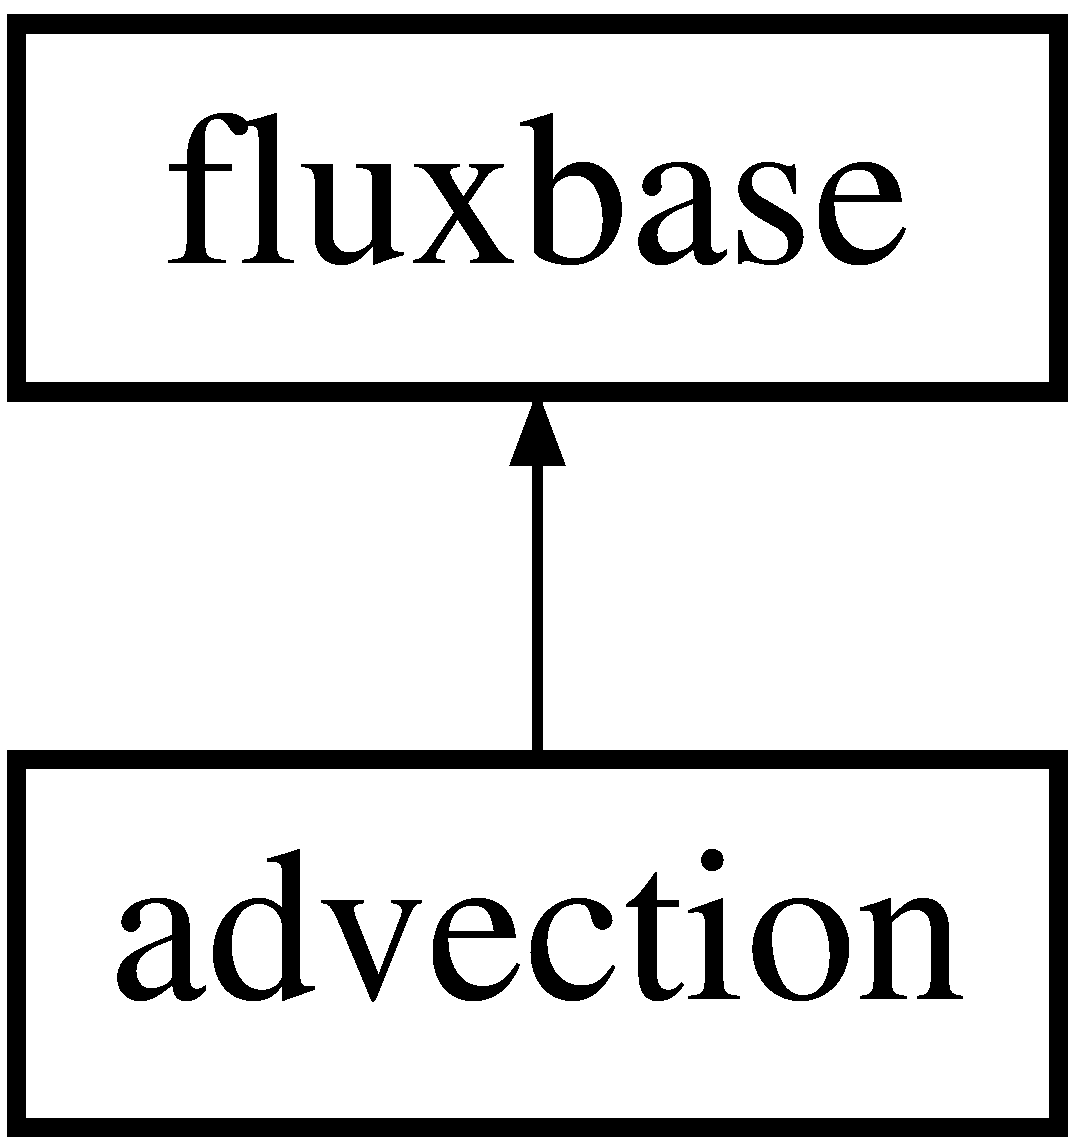
\includegraphics[height=2.000000cm]{classadvection}
\end{center}
\end{figure}
\subsection*{Public Member Functions}
\begin{DoxyCompactItemize}
\item 
double {\bf eval} (double $\ast$, double $\ast$, double $\ast$, double $\ast$, double $\ast$)
\begin{DoxyCompactList}\small\item\em Evaluation of the advection flux. \end{DoxyCompactList}\item 
void {\bf eval\-\_\-l} (double $\ast$, double $\ast$, double $\ast$, double $\ast$, double $\ast$)
\begin{DoxyCompactList}\small\item\em Virtual non conservative evaluation of the flux on the left of the element. \end{DoxyCompactList}\item 
void {\bf eval\-\_\-r} (double $\ast$, double $\ast$, double $\ast$, double $\ast$, double $\ast$)
\begin{DoxyCompactList}\small\item\em Virtual non conservative evaluation of the flux on the right of the element. \end{DoxyCompactList}\end{DoxyCompactItemize}


\subsection{Detailed Description}
Derived fluxbase class for Advection. 

\subsection{Member Function Documentation}
\index{advection@{advection}!eval@{eval}}
\index{eval@{eval}!advection@{advection}}
\subsubsection[{eval}]{\setlength{\rightskip}{0pt plus 5cm}double advection\-::eval (
\begin{DoxyParamCaption}
\item[{double $\ast$}]{F, }
\item[{double $\ast$}]{u\-L, }
\item[{double $\ast$}]{u\-R, }
\item[{double $\ast$}]{q\-L, }
\item[{double $\ast$}]{q\-R}
\end{DoxyParamCaption}
)\hspace{0.3cm}{\ttfamily [virtual]}}\label{classadvection_a39ffeff22d8c4bab9b209305e9c2ff05}


Evaluation of the advection flux. 



Implements {\bf fluxbase} \doxyref{}{p.}{classfluxbase_ab41e8752c750488dbcbc8ef24e277110}.



References a, advection\-\_\-speed, and element\-::systemsize1.

\index{advection@{advection}!eval\-\_\-l@{eval\-\_\-l}}
\index{eval\-\_\-l@{eval\-\_\-l}!advection@{advection}}
\subsubsection[{eval\-\_\-l}]{\setlength{\rightskip}{0pt plus 5cm}void advection\-::eval\-\_\-l (
\begin{DoxyParamCaption}
\item[{double $\ast$}]{, }
\item[{double $\ast$}]{, }
\item[{double $\ast$}]{, }
\item[{double $\ast$}]{, }
\item[{double $\ast$}]{}
\end{DoxyParamCaption}
)\hspace{0.3cm}{\ttfamily [inline]}, {\ttfamily [virtual]}}\label{classadvection_a64544ecc593a0e2d9e53c80cddce46fd}


Virtual non conservative evaluation of the flux on the left of the element. 



Implements {\bf fluxbase} \doxyref{}{p.}{classfluxbase_a184e5d5629191871c6dd9cd6b4e82799}.

\index{advection@{advection}!eval\-\_\-r@{eval\-\_\-r}}
\index{eval\-\_\-r@{eval\-\_\-r}!advection@{advection}}
\subsubsection[{eval\-\_\-r}]{\setlength{\rightskip}{0pt plus 5cm}void advection\-::eval\-\_\-r (
\begin{DoxyParamCaption}
\item[{double $\ast$}]{, }
\item[{double $\ast$}]{, }
\item[{double $\ast$}]{, }
\item[{double $\ast$}]{, }
\item[{double $\ast$}]{}
\end{DoxyParamCaption}
)\hspace{0.3cm}{\ttfamily [inline]}, {\ttfamily [virtual]}}\label{classadvection_a17852fcad013696082568c732fe89003}


Virtual non conservative evaluation of the flux on the right of the element. 



Implements {\bf fluxbase} \doxyref{}{p.}{classfluxbase_ab5e6afaa22aff4a1bbbce0bba561fed3}.



The documentation for this class was generated from the following files\-:\begin{DoxyCompactItemize}
\item 
{\bf flux.\-h}\item 
{\bf flux.\-cpp}\end{DoxyCompactItemize}

\section{burgers Class Reference}
\label{classburgers}\index{burgers@{burgers}}


Derived fluxbase class for Burgers' equation.  




{\ttfamily \#include $<$flux.\-h$>$}

Inheritance diagram for burgers\-:\begin{figure}[H]
\begin{center}
\leavevmode
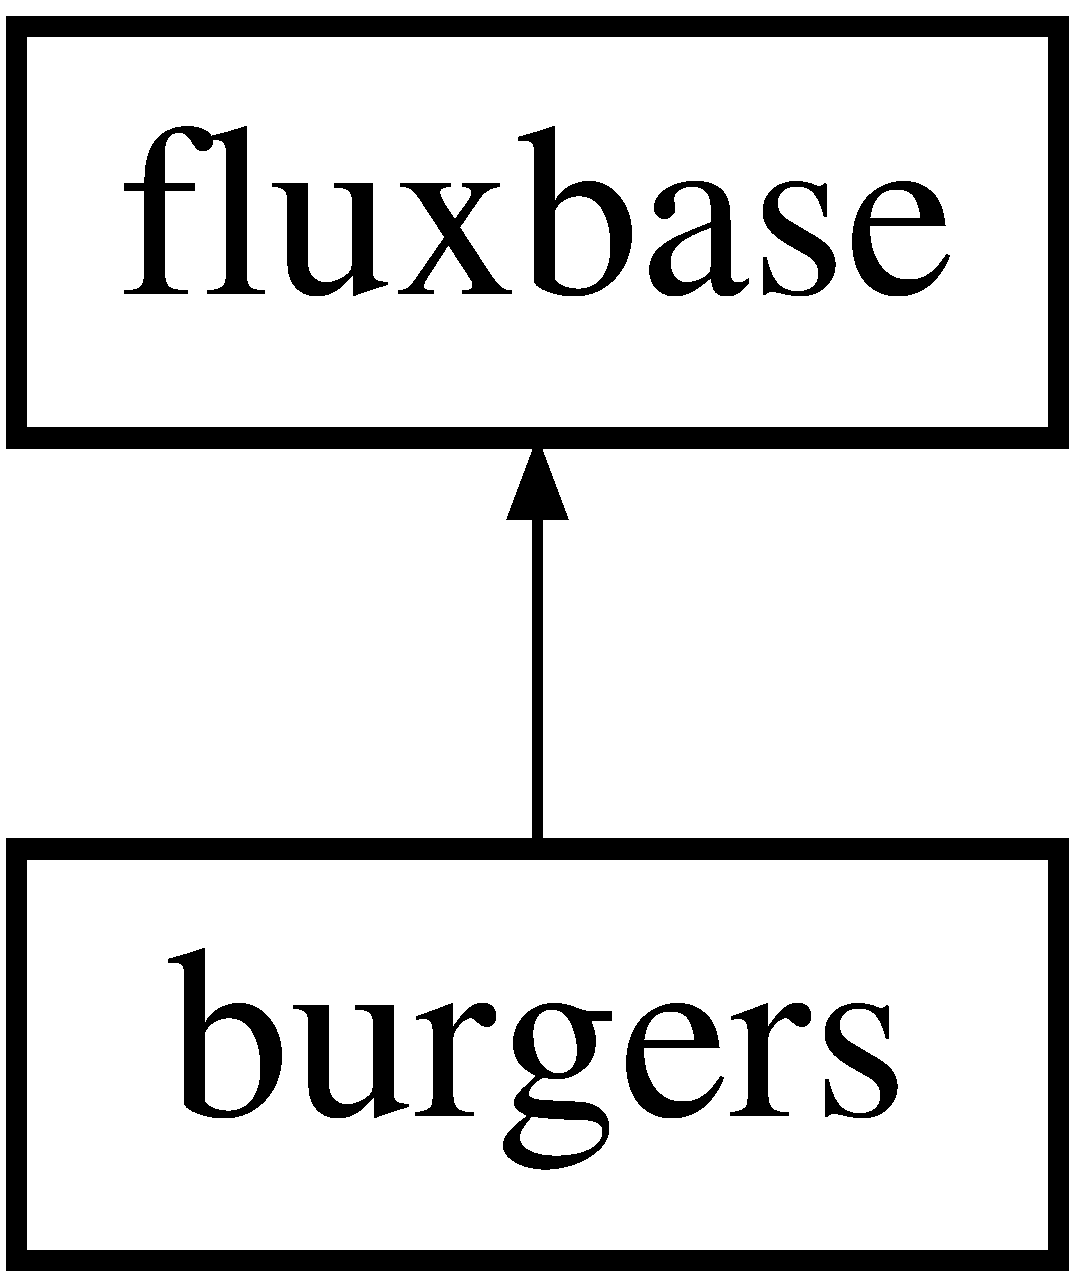
\includegraphics[height=2.000000cm]{classburgers}
\end{center}
\end{figure}
\subsection*{Public Member Functions}
\begin{DoxyCompactItemize}
\item 
double {\bf eval} (double $\ast$, double $\ast$, double $\ast$, double $\ast$, double $\ast$)
\begin{DoxyCompactList}\small\item\em Evaluation of the flux for Burgers' equation. \end{DoxyCompactList}\item 
void {\bf eval\-\_\-l} (double $\ast$, double $\ast$, double $\ast$, double $\ast$, double $\ast$)
\begin{DoxyCompactList}\small\item\em Virtual non conservative evaluation of the flux on the left of the element. \end{DoxyCompactList}\item 
void {\bf eval\-\_\-r} (double $\ast$, double $\ast$, double $\ast$, double $\ast$, double $\ast$)
\begin{DoxyCompactList}\small\item\em Virtual non conservative evaluation of the flux on the right of the element. \end{DoxyCompactList}\end{DoxyCompactItemize}


\subsection{Detailed Description}
Derived fluxbase class for Burgers' equation. 

\subsection{Member Function Documentation}
\index{burgers@{burgers}!eval@{eval}}
\index{eval@{eval}!burgers@{burgers}}
\subsubsection[{eval}]{\setlength{\rightskip}{0pt plus 5cm}double burgers\-::eval (
\begin{DoxyParamCaption}
\item[{double $\ast$}]{F, }
\item[{double $\ast$}]{u\-L, }
\item[{double $\ast$}]{u\-R, }
\item[{double $\ast$}]{q\-L, }
\item[{double $\ast$}]{q\-R}
\end{DoxyParamCaption}
)\hspace{0.3cm}{\ttfamily [virtual]}}\label{classburgers_a0f757dbcb4dc096dc7d44a32b0a7a7df}


Evaluation of the flux for Burgers' equation. 



Implements {\bf fluxbase} \doxyref{}{p.}{classfluxbase_ab41e8752c750488dbcbc8ef24e277110}.



References element\-::systemsize1.

\index{burgers@{burgers}!eval\-\_\-l@{eval\-\_\-l}}
\index{eval\-\_\-l@{eval\-\_\-l}!burgers@{burgers}}
\subsubsection[{eval\-\_\-l}]{\setlength{\rightskip}{0pt plus 5cm}void burgers\-::eval\-\_\-l (
\begin{DoxyParamCaption}
\item[{double $\ast$}]{, }
\item[{double $\ast$}]{, }
\item[{double $\ast$}]{, }
\item[{double $\ast$}]{, }
\item[{double $\ast$}]{}
\end{DoxyParamCaption}
)\hspace{0.3cm}{\ttfamily [inline]}, {\ttfamily [virtual]}}\label{classburgers_ad2ecdd94d31dd2bbf4accdde9967e25e}


Virtual non conservative evaluation of the flux on the left of the element. 



Implements {\bf fluxbase} \doxyref{}{p.}{classfluxbase_a184e5d5629191871c6dd9cd6b4e82799}.

\index{burgers@{burgers}!eval\-\_\-r@{eval\-\_\-r}}
\index{eval\-\_\-r@{eval\-\_\-r}!burgers@{burgers}}
\subsubsection[{eval\-\_\-r}]{\setlength{\rightskip}{0pt plus 5cm}void burgers\-::eval\-\_\-r (
\begin{DoxyParamCaption}
\item[{double $\ast$}]{, }
\item[{double $\ast$}]{, }
\item[{double $\ast$}]{, }
\item[{double $\ast$}]{, }
\item[{double $\ast$}]{}
\end{DoxyParamCaption}
)\hspace{0.3cm}{\ttfamily [inline]}, {\ttfamily [virtual]}}\label{classburgers_ae0a45d14818eed9d9df8236e6bf6e2b0}


Virtual non conservative evaluation of the flux on the right of the element. 



Implements {\bf fluxbase} \doxyref{}{p.}{classfluxbase_ab5e6afaa22aff4a1bbbce0bba561fed3}.



The documentation for this class was generated from the following files\-:\begin{DoxyCompactItemize}
\item 
{\bf flux.\-h}\item 
{\bf flux.\-cpp}\end{DoxyCompactItemize}

\section{burgersdiffusion Class Reference}
\label{classburgersdiffusion}\index{burgersdiffusion@{burgersdiffusion}}


Derived fluxbase class for Burgers' equation.  




{\ttfamily \#include $<$flux.\-h$>$}

Inheritance diagram for burgersdiffusion\-:\begin{figure}[H]
\begin{center}
\leavevmode
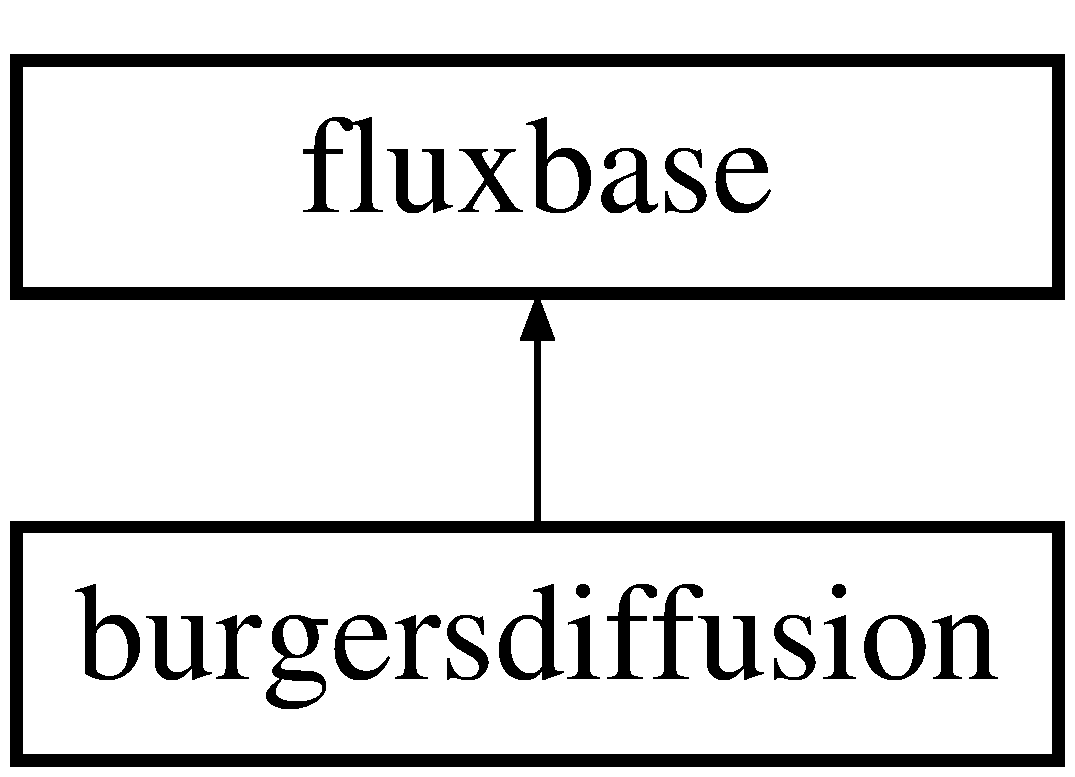
\includegraphics[height=2.000000cm]{classburgersdiffusion}
\end{center}
\end{figure}
\subsection*{Public Member Functions}
\begin{DoxyCompactItemize}
\item 
double {\bf eval} (double $\ast$, double $\ast$, double $\ast$, double $\ast$, double $\ast$)
\begin{DoxyCompactList}\small\item\em Evaluation of the flux for Burgers' equation including diffusion. \end{DoxyCompactList}\item 
void {\bf eval\-\_\-l} (double $\ast$, double $\ast$, double $\ast$, double $\ast$, double $\ast$)
\begin{DoxyCompactList}\small\item\em Virtual non conservative evaluation of the flux on the left of the element. \end{DoxyCompactList}\item 
void {\bf eval\-\_\-r} (double $\ast$, double $\ast$, double $\ast$, double $\ast$, double $\ast$)
\begin{DoxyCompactList}\small\item\em Virtual non conservative evaluation of the flux on the right of the element. \end{DoxyCompactList}\end{DoxyCompactItemize}


\subsection{Detailed Description}
Derived fluxbase class for Burgers' equation. 

\subsection{Member Function Documentation}
\index{burgersdiffusion@{burgersdiffusion}!eval@{eval}}
\index{eval@{eval}!burgersdiffusion@{burgersdiffusion}}
\subsubsection[{eval}]{\setlength{\rightskip}{0pt plus 5cm}double burgersdiffusion\-::eval (
\begin{DoxyParamCaption}
\item[{double $\ast$}]{F, }
\item[{double $\ast$}]{u\-L, }
\item[{double $\ast$}]{u\-R, }
\item[{double $\ast$}]{q\-L, }
\item[{double $\ast$}]{q\-R}
\end{DoxyParamCaption}
)\hspace{0.3cm}{\ttfamily [virtual]}}\label{classburgersdiffusion_abb97ec0449cd1c0a8ad476b7de3a62a9}


Evaluation of the flux for Burgers' equation including diffusion. 



Implements {\bf fluxbase} \doxyref{}{p.}{classfluxbase_ab41e8752c750488dbcbc8ef24e277110}.



References element\-::systemsize1.

\index{burgersdiffusion@{burgersdiffusion}!eval\-\_\-l@{eval\-\_\-l}}
\index{eval\-\_\-l@{eval\-\_\-l}!burgersdiffusion@{burgersdiffusion}}
\subsubsection[{eval\-\_\-l}]{\setlength{\rightskip}{0pt plus 5cm}void burgersdiffusion\-::eval\-\_\-l (
\begin{DoxyParamCaption}
\item[{double $\ast$}]{, }
\item[{double $\ast$}]{, }
\item[{double $\ast$}]{, }
\item[{double $\ast$}]{, }
\item[{double $\ast$}]{}
\end{DoxyParamCaption}
)\hspace{0.3cm}{\ttfamily [inline]}, {\ttfamily [virtual]}}\label{classburgersdiffusion_a0ba7b3bc143ecd0cfb40431f957dc552}


Virtual non conservative evaluation of the flux on the left of the element. 



Implements {\bf fluxbase} \doxyref{}{p.}{classfluxbase_a184e5d5629191871c6dd9cd6b4e82799}.

\index{burgersdiffusion@{burgersdiffusion}!eval\-\_\-r@{eval\-\_\-r}}
\index{eval\-\_\-r@{eval\-\_\-r}!burgersdiffusion@{burgersdiffusion}}
\subsubsection[{eval\-\_\-r}]{\setlength{\rightskip}{0pt plus 5cm}void burgersdiffusion\-::eval\-\_\-r (
\begin{DoxyParamCaption}
\item[{double $\ast$}]{, }
\item[{double $\ast$}]{, }
\item[{double $\ast$}]{, }
\item[{double $\ast$}]{, }
\item[{double $\ast$}]{}
\end{DoxyParamCaption}
)\hspace{0.3cm}{\ttfamily [inline]}, {\ttfamily [virtual]}}\label{classburgersdiffusion_aa369a3cc470f23bb10b9415efb27b677}


Virtual non conservative evaluation of the flux on the right of the element. 



Implements {\bf fluxbase} \doxyref{}{p.}{classfluxbase_ab5e6afaa22aff4a1bbbce0bba561fed3}.



The documentation for this class was generated from the following files\-:\begin{DoxyCompactItemize}
\item 
{\bf flux.\-h}\item 
{\bf flux.\-cpp}\end{DoxyCompactItemize}

\section{diffusion Class Reference}
\label{classdiffusion}\index{diffusion@{diffusion}}


L\-D\-G diffusion flux class used in comination with Burgers' equation.  




{\ttfamily \#include $<$flux2.\-h$>$}

Inheritance diagram for diffusion\-:\begin{figure}[H]
\begin{center}
\leavevmode
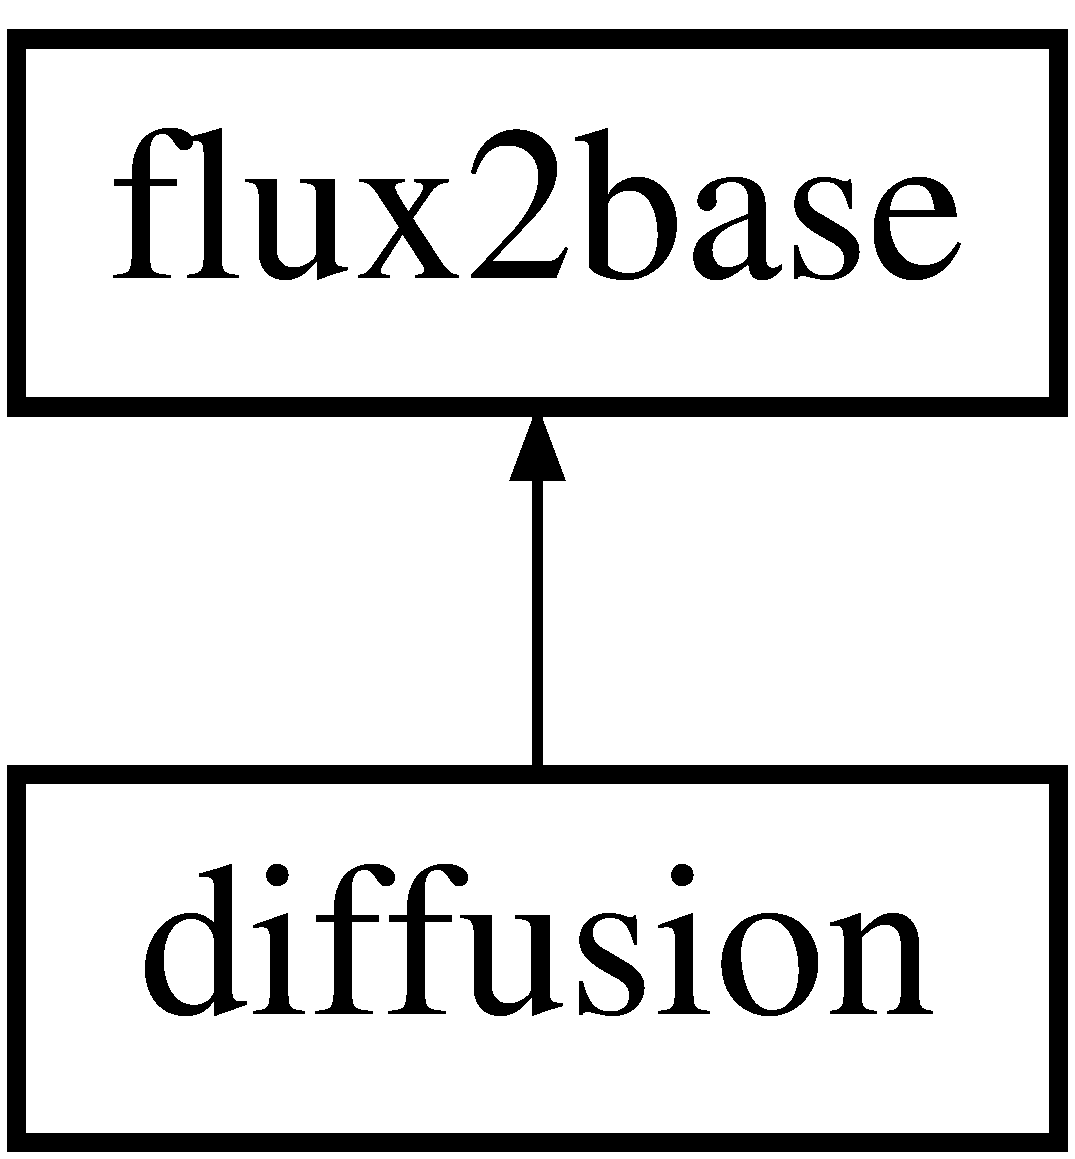
\includegraphics[height=2.000000cm]{classdiffusion}
\end{center}
\end{figure}
\subsection*{Public Member Functions}
\begin{DoxyCompactItemize}
\item 
double {\bf eval} (double $\ast$, double $\ast$, double $\ast$)
\begin{DoxyCompactList}\small\item\em Evaluates the flux for the L\-D\-G variables for the difussion. \end{DoxyCompactList}\end{DoxyCompactItemize}


\subsection{Detailed Description}
L\-D\-G diffusion flux class used in comination with Burgers' equation. 

\subsection{Member Function Documentation}
\index{diffusion@{diffusion}!eval@{eval}}
\index{eval@{eval}!diffusion@{diffusion}}
\subsubsection[{eval}]{\setlength{\rightskip}{0pt plus 5cm}double diffusion\-::eval (
\begin{DoxyParamCaption}
\item[{double $\ast$}]{F, }
\item[{double $\ast$}]{u\-L, }
\item[{double $\ast$}]{u\-R}
\end{DoxyParamCaption}
)\hspace{0.3cm}{\ttfamily [virtual]}}\label{classdiffusion_a998c0963f4273bdb1b81e434501caf7e}


Evaluates the flux for the L\-D\-G variables for the difussion. 



Implements {\bf flux2base} \doxyref{}{p.}{classflux2base_a4ecfc0d7470722ef299fa054c926f540}.



References element\-::systemsize2.



The documentation for this class was generated from the following files\-:\begin{DoxyCompactItemize}
\item 
{\bf flux2.\-h}\item 
{\bf flux2.\-cpp}\end{DoxyCompactItemize}

\section{element Class Reference}
\label{classelement}\index{element@{element}}


The element class.  




{\ttfamily \#include $<$element.\-h$>$}

\subsection*{Public Member Functions}
\begin{DoxyCompactItemize}
\item 
{\bf element} ()
\begin{DoxyCompactList}\small\item\em Default constructor. \end{DoxyCompactList}\item 
{\bf element} (int, int, double)
\begin{DoxyCompactList}\small\item\em Overloaded constructor. \end{DoxyCompactList}\item 
void {\bf updateu} ()
\begin{DoxyCompactList}\small\item\em Updates u1, u2, u1slope and u2slope in each time step. \end{DoxyCompactList}\item 
void {\bf updateq} ()
\begin{DoxyCompactList}\small\item\em Updates q1 and q2 in every time step. \end{DoxyCompactList}\item 
{\bf $\sim$element} ()
\begin{DoxyCompactList}\small\item\em Default destructor. \end{DoxyCompactList}\end{DoxyCompactItemize}
\subsection*{Public Attributes}
\begin{DoxyCompactItemize}
\item 
int {\bf Node1}
\begin{DoxyCompactList}\small\item\em The node numbers which bound the element. \end{DoxyCompactList}\item 
int {\bf Node2}
\item 
double {\bf length}
\begin{DoxyCompactList}\small\item\em The length of the element. \end{DoxyCompactList}\item 
{\bf state} $\ast$ {\bf U}
\begin{DoxyCompactList}\small\item\em The stored Discontinuous Galerkin variables. \end{DoxyCompactList}\item 
{\bf state} $\ast$ {\bf R\-H\-Sof\-U}
\begin{DoxyCompactList}\small\item\em The right hand side used while calculating one time step. \end{DoxyCompactList}\item 
{\bf state} $\ast$ {\bf U\-\_\-old}
\begin{DoxyCompactList}\small\item\em A backup of U needed for some time integration schemes. \end{DoxyCompactList}\item 
{\bf state} $\ast$ {\bf R\-H\-Sof\-U\-\_\-old}
\begin{DoxyCompactList}\small\item\em A backup of R\-H\-Sof\-U needed for some time integration schemes. \end{DoxyCompactList}\item 
{\bf state} $\ast$ {\bf Q}
\begin{DoxyCompactList}\small\item\em The Local Discontinuous Galerkin variables. \end{DoxyCompactList}\item 
{\bf state} $\ast$ {\bf R\-H\-Sof\-Q}
\begin{DoxyCompactList}\small\item\em The right hand side used for Local Discontinuous Galerkin calculations. \end{DoxyCompactList}\item 
{\bf state} {\bf Stab\-Op}
\begin{DoxyCompactList}\small\item\em The value of the stabilisation operator. \end{DoxyCompactList}\item 
{\bf state} {\bf Stab\-Op\-\_\-old}
\begin{DoxyCompactList}\small\item\em A backup of the stabilisation operator used in some time integration schemes. \end{DoxyCompactList}\item 
double {\bf Kriv}
\begin{DoxyCompactList}\small\item\em Discontinuity detector variable from Krividonova et al., 2004. \end{DoxyCompactList}\item 
int {\bf Kriv\-Count}
\begin{DoxyCompactList}\small\item\em Count of how many faces have information which passes into the cell $\| \partial\Omega^- \|$. \end{DoxyCompactList}\item 
double {\bf ws}
\begin{DoxyCompactList}\small\item\em The maximum wavespeed sorted per element used to determine the time step. \end{DoxyCompactList}\item 
double {\bf dds}
\begin{DoxyCompactList}\small\item\em The maximum d\-\_\-xx wavespeed sorted per element used to determine the time step. \end{DoxyCompactList}\item 
double $\ast$ {\bf u1}
\begin{DoxyCompactList}\small\item\em The values of the D\-G variables in -\/ep. \end{DoxyCompactList}\item 
double $\ast$ {\bf u2}
\begin{DoxyCompactList}\small\item\em The values of the D\-G variables in ep. \end{DoxyCompactList}\item 
double $\ast$ {\bf u1slope}
\begin{DoxyCompactList}\small\item\em The values of slopes of the D\-G variables in -\/ep. \end{DoxyCompactList}\item 
double $\ast$ {\bf u2slope}
\begin{DoxyCompactList}\small\item\em The values of slopes of the D\-G variables in ep. \end{DoxyCompactList}\item 
double $\ast$ {\bf q1}
\begin{DoxyCompactList}\small\item\em The values of the L\-D\-G variables in -\/ep. \end{DoxyCompactList}\item 
double $\ast$ {\bf q2}
\begin{DoxyCompactList}\small\item\em The values of the L\-D\-G variables in -\/ep. \end{DoxyCompactList}\end{DoxyCompactItemize}
\subsection*{Static Public Attributes}
\begin{DoxyCompactItemize}
\item 
static int {\bf systemsize1}
\begin{DoxyCompactList}\small\item\em The dimension of the Discontinuous Galerkin variables. \end{DoxyCompactList}\item 
static int {\bf systemsize2}
\begin{DoxyCompactList}\small\item\em The dimension of the Local Discontinuous Galerkin variables. \end{DoxyCompactList}\item 
static double {\bf ep} = 1.\-0/sqrt(3.\-0)
\begin{DoxyCompactList}\small\item\em Interpolation point used for two point Gaussian quadrature. \end{DoxyCompactList}\item 
static double {\bf C\-F\-L}
\begin{DoxyCompactList}\small\item\em The Courant coefficient number. \end{DoxyCompactList}\end{DoxyCompactItemize}


\subsection{Detailed Description}
The element class. 

The element class is the building block of how the information per element is stored. 

\subsection{Constructor \& Destructor Documentation}
\index{element@{element}!element@{element}}
\index{element@{element}!element@{element}}
\subsubsection[{element}]{\setlength{\rightskip}{0pt plus 5cm}element\-::element (
\begin{DoxyParamCaption}
{}
\end{DoxyParamCaption}
)}\label{classelement_ab855762fbfbeb7307a78943b10c3afbb}


Default constructor. 

\index{element@{element}!element@{element}}
\index{element@{element}!element@{element}}
\subsubsection[{element}]{\setlength{\rightskip}{0pt plus 5cm}element\-::element (
\begin{DoxyParamCaption}
\item[{int}]{value1, }
\item[{int}]{value2, }
\item[{double}]{value3}
\end{DoxyParamCaption}
)}\label{classelement_afae6e952256e36fe5836b24af2c5509c}


Overloaded constructor. 



References systemsize1, and systemsize2.

\index{element@{element}!$\sim$element@{$\sim$element}}
\index{$\sim$element@{$\sim$element}!element@{element}}
\subsubsection[{$\sim$element}]{\setlength{\rightskip}{0pt plus 5cm}element\-::$\sim$element (
\begin{DoxyParamCaption}
{}
\end{DoxyParamCaption}
)}\label{classelement_ab986cb2721f12b05716a9f2eb583a840}


Default destructor. 



\subsection{Member Function Documentation}
\index{element@{element}!updateq@{updateq}}
\index{updateq@{updateq}!element@{element}}
\subsubsection[{updateq}]{\setlength{\rightskip}{0pt plus 5cm}void element\-::updateq (
\begin{DoxyParamCaption}
{}
\end{DoxyParamCaption}
)}\label{classelement_a749ff1b33a374f49d8816e63d48b9770}


Updates q1 and q2 in every time step. 

Loop over the variables.

Determine the new values at +ep and -\/ep. 

References systemsize2.

\index{element@{element}!updateu@{updateu}}
\index{updateu@{updateu}!element@{element}}
\subsubsection[{updateu}]{\setlength{\rightskip}{0pt plus 5cm}void element\-::updateu (
\begin{DoxyParamCaption}
{}
\end{DoxyParamCaption}
)}\label{classelement_a9d4be14ea3bb6fecd86ace1fbfa2899d}


Updates u1, u2, u1slope and u2slope in each time step. 

Loop over the variables.

Determine the new values at +ep and -\/ep. 

References systemsize1.



\subsection{Member Data Documentation}
\index{element@{element}!C\-F\-L@{C\-F\-L}}
\index{C\-F\-L@{C\-F\-L}!element@{element}}
\subsubsection[{C\-F\-L}]{\setlength{\rightskip}{0pt plus 5cm}double element\-::\-C\-F\-L\hspace{0.3cm}{\ttfamily [static]}}\label{classelement_abd301c7f64d964fb0b276d23989b2e79}


The Courant coefficient number. 



Referenced by main().

\index{element@{element}!dds@{dds}}
\index{dds@{dds}!element@{element}}
\subsubsection[{dds}]{\setlength{\rightskip}{0pt plus 5cm}double element\-::dds}\label{classelement_a2cff653cbc92e0ee758478899d177b4e}


The maximum d\-\_\-xx wavespeed sorted per element used to determine the time step. 

\index{element@{element}!ep@{ep}}
\index{ep@{ep}!element@{element}}
\subsubsection[{ep}]{\setlength{\rightskip}{0pt plus 5cm}double element\-::ep = 1.\-0/sqrt(3.\-0)\hspace{0.3cm}{\ttfamily [static]}}\label{classelement_a38e6f5a1b5f9f18348dbc73c55b01dd8}


Interpolation point used for two point Gaussian quadrature. 



Referenced by sourceproc().

\index{element@{element}!Kriv@{Kriv}}
\index{Kriv@{Kriv}!element@{element}}
\subsubsection[{Kriv}]{\setlength{\rightskip}{0pt plus 5cm}double element\-::\-Kriv}\label{classelement_abe57494fc7bfc89bde32781336cca651}


Discontinuity detector variable from Krividonova et al., 2004. 

\index{element@{element}!Kriv\-Count@{Kriv\-Count}}
\index{Kriv\-Count@{Kriv\-Count}!element@{element}}
\subsubsection[{Kriv\-Count}]{\setlength{\rightskip}{0pt plus 5cm}int element\-::\-Kriv\-Count}\label{classelement_ab8b596c587764a871d0ad0ec9e01636d}


Count of how many faces have information which passes into the cell $\| \partial\Omega^- \|$. 

\index{element@{element}!length@{length}}
\index{length@{length}!element@{element}}
\subsubsection[{length}]{\setlength{\rightskip}{0pt plus 5cm}double element\-::length}\label{classelement_a06670ef1299084fc645fc1441ee9fe62}


The length of the element. 

\index{element@{element}!Node1@{Node1}}
\index{Node1@{Node1}!element@{element}}
\subsubsection[{Node1}]{\setlength{\rightskip}{0pt plus 5cm}int element\-::\-Node1}\label{classelement_a39288677ba181a95c92cdb269947cfac}


The node numbers which bound the element. 

\index{element@{element}!Node2@{Node2}}
\index{Node2@{Node2}!element@{element}}
\subsubsection[{Node2}]{\setlength{\rightskip}{0pt plus 5cm}int element\-::\-Node2}\label{classelement_a30ebcc5c6f8e8a4ab3f960da1ec410d1}
\index{element@{element}!Q@{Q}}
\index{Q@{Q}!element@{element}}
\subsubsection[{Q}]{\setlength{\rightskip}{0pt plus 5cm}{\bf state}$\ast$ element\-::\-Q}\label{classelement_aa83f5142f575c2bc3504cf25e8749ab6}


The Local Discontinuous Galerkin variables. 

\index{element@{element}!q1@{q1}}
\index{q1@{q1}!element@{element}}
\subsubsection[{q1}]{\setlength{\rightskip}{0pt plus 5cm}double$\ast$ element\-::q1}\label{classelement_afee2741280acb7f07e4d97e3d319f85b}


The values of the L\-D\-G variables in -\/ep. 

\index{element@{element}!q2@{q2}}
\index{q2@{q2}!element@{element}}
\subsubsection[{q2}]{\setlength{\rightskip}{0pt plus 5cm}double$\ast$ element\-::q2}\label{classelement_afc7fe8e8ea7c9152dbf462a8a4d165af}


The values of the L\-D\-G variables in -\/ep. 

\index{element@{element}!R\-H\-Sof\-Q@{R\-H\-Sof\-Q}}
\index{R\-H\-Sof\-Q@{R\-H\-Sof\-Q}!element@{element}}
\subsubsection[{R\-H\-Sof\-Q}]{\setlength{\rightskip}{0pt plus 5cm}{\bf state}$\ast$ element\-::\-R\-H\-Sof\-Q}\label{classelement_a51050bbe3d8c2823a28a245601cd13fd}


The right hand side used for Local Discontinuous Galerkin calculations. 

\index{element@{element}!R\-H\-Sof\-U@{R\-H\-Sof\-U}}
\index{R\-H\-Sof\-U@{R\-H\-Sof\-U}!element@{element}}
\subsubsection[{R\-H\-Sof\-U}]{\setlength{\rightskip}{0pt plus 5cm}{\bf state}$\ast$ element\-::\-R\-H\-Sof\-U}\label{classelement_ad30a3bbb3101ee29d089fe12cc8302fd}


The right hand side used while calculating one time step. 

\index{element@{element}!R\-H\-Sof\-U\-\_\-old@{R\-H\-Sof\-U\-\_\-old}}
\index{R\-H\-Sof\-U\-\_\-old@{R\-H\-Sof\-U\-\_\-old}!element@{element}}
\subsubsection[{R\-H\-Sof\-U\-\_\-old}]{\setlength{\rightskip}{0pt plus 5cm}{\bf state}$\ast$ element\-::\-R\-H\-Sof\-U\-\_\-old}\label{classelement_ae661a551143416f6b60b2c43890cd8e3}


A backup of R\-H\-Sof\-U needed for some time integration schemes. 

\index{element@{element}!Stab\-Op@{Stab\-Op}}
\index{Stab\-Op@{Stab\-Op}!element@{element}}
\subsubsection[{Stab\-Op}]{\setlength{\rightskip}{0pt plus 5cm}{\bf state} element\-::\-Stab\-Op}\label{classelement_ae98a7807eda38e991af4be3c9a2f3049}


The value of the stabilisation operator. 

\index{element@{element}!Stab\-Op\-\_\-old@{Stab\-Op\-\_\-old}}
\index{Stab\-Op\-\_\-old@{Stab\-Op\-\_\-old}!element@{element}}
\subsubsection[{Stab\-Op\-\_\-old}]{\setlength{\rightskip}{0pt plus 5cm}{\bf state} element\-::\-Stab\-Op\-\_\-old}\label{classelement_adb01f777e07f9049787784e9e3cb03f9}


A backup of the stabilisation operator used in some time integration schemes. 

\index{element@{element}!systemsize1@{systemsize1}}
\index{systemsize1@{systemsize1}!element@{element}}
\subsubsection[{systemsize1}]{\setlength{\rightskip}{0pt plus 5cm}int element\-::systemsize1\hspace{0.3cm}{\ttfamily [static]}}\label{classelement_ab273d8a7b662315d58ed949018e26ed2}


The dimension of the Discontinuous Galerkin variables. 



Referenced by cranknicolsonwp(), element(), eulerforw(), topography\-::eval(), advection\-::eval(), exchange\-::eval(), burgers\-::eval(), burgersdiffusion\-::eval(), swehllc\-::eval(), swehllctopography\-::eval(), sedimenttransport\-::eval(), grassburgers\-::eval(), suspendedsediment\-::eval(), swehllctopography\-::eval\-\_\-l(), sedimenttransport\-::eval\-\_\-l(), lfgrassmomentum\-::eval\-\_\-l(), suspendedsediment\-::eval\-\_\-l(), lfgrassmomentumdiffusion\-::eval\-\_\-l(), swehllctopography\-::eval\-\_\-r(), sedimenttransport\-::eval\-\_\-r(), lfgrassmomentum\-::eval\-\_\-r(), suspendedsediment\-::eval\-\_\-r(), lfgrassmomentumdiffusion\-::eval\-\_\-r(), flux2proc(), fluxproc(), initcon(), main(), node\-::node(), output(), rk3(), sourceproc(), updatenodesu(), and updateu().

\index{element@{element}!systemsize2@{systemsize2}}
\index{systemsize2@{systemsize2}!element@{element}}
\subsubsection[{systemsize2}]{\setlength{\rightskip}{0pt plus 5cm}int element\-::systemsize2\hspace{0.3cm}{\ttfamily [static]}}\label{classelement_a32e743b830c5d986454bbcfe7911ce30}


The dimension of the Local Discontinuous Galerkin variables. 



Referenced by cranknicolsonwp(), element(), eulerforw(), diffusion\-::eval(), sedimentdiffusion\-::eval(), flux2proc(), main(), node\-::node(), output(), rk3(), updatenodesq(), and updateq().

\index{element@{element}!U@{U}}
\index{U@{U}!element@{element}}
\subsubsection[{U}]{\setlength{\rightskip}{0pt plus 5cm}{\bf state}$\ast$ element\-::\-U}\label{classelement_ab5bba2272163b3ac622f4de3293da7de}


The stored Discontinuous Galerkin variables. 

\index{element@{element}!u1@{u1}}
\index{u1@{u1}!element@{element}}
\subsubsection[{u1}]{\setlength{\rightskip}{0pt plus 5cm}double$\ast$ element\-::u1}\label{classelement_a35bc049ae767ff3bb3ace6983d8a22a7}


The values of the D\-G variables in -\/ep. 

\index{element@{element}!u1slope@{u1slope}}
\index{u1slope@{u1slope}!element@{element}}
\subsubsection[{u1slope}]{\setlength{\rightskip}{0pt plus 5cm}double$\ast$ element\-::u1slope}\label{classelement_ae9779e7ddf4675c3a7ef3a5955aa613c}


The values of slopes of the D\-G variables in -\/ep. 

\index{element@{element}!u2@{u2}}
\index{u2@{u2}!element@{element}}
\subsubsection[{u2}]{\setlength{\rightskip}{0pt plus 5cm}double$\ast$ element\-::u2}\label{classelement_ad58036341aac37c97cb81d28f5e26409}


The values of the D\-G variables in ep. 

\index{element@{element}!u2slope@{u2slope}}
\index{u2slope@{u2slope}!element@{element}}
\subsubsection[{u2slope}]{\setlength{\rightskip}{0pt plus 5cm}double$\ast$ element\-::u2slope}\label{classelement_a7488ad853e91d10a94afbdd7b0450682}


The values of slopes of the D\-G variables in ep. 

\index{element@{element}!U\-\_\-old@{U\-\_\-old}}
\index{U\-\_\-old@{U\-\_\-old}!element@{element}}
\subsubsection[{U\-\_\-old}]{\setlength{\rightskip}{0pt plus 5cm}{\bf state}$\ast$ element\-::\-U\-\_\-old}\label{classelement_a7c6730d8fb495e959b0479f2c6a21d9d}


A backup of U needed for some time integration schemes. 

\index{element@{element}!ws@{ws}}
\index{ws@{ws}!element@{element}}
\subsubsection[{ws}]{\setlength{\rightskip}{0pt plus 5cm}double element\-::ws}\label{classelement_a9b99359b392c0e02a7706cd447f8b82d}


The maximum wavespeed sorted per element used to determine the time step. 



The documentation for this class was generated from the following files\-:\begin{DoxyCompactItemize}
\item 
{\bf element.\-h}\item 
{\bf element.\-cpp}\end{DoxyCompactItemize}

\section{exchange Class Reference}
\label{classexchange}\index{exchange@{exchange}}


Derived Exchange Class from Source\-Base.  




{\ttfamily \#include $<$source.\-h$>$}

Inheritance diagram for exchange\-:\begin{figure}[H]
\begin{center}
\leavevmode
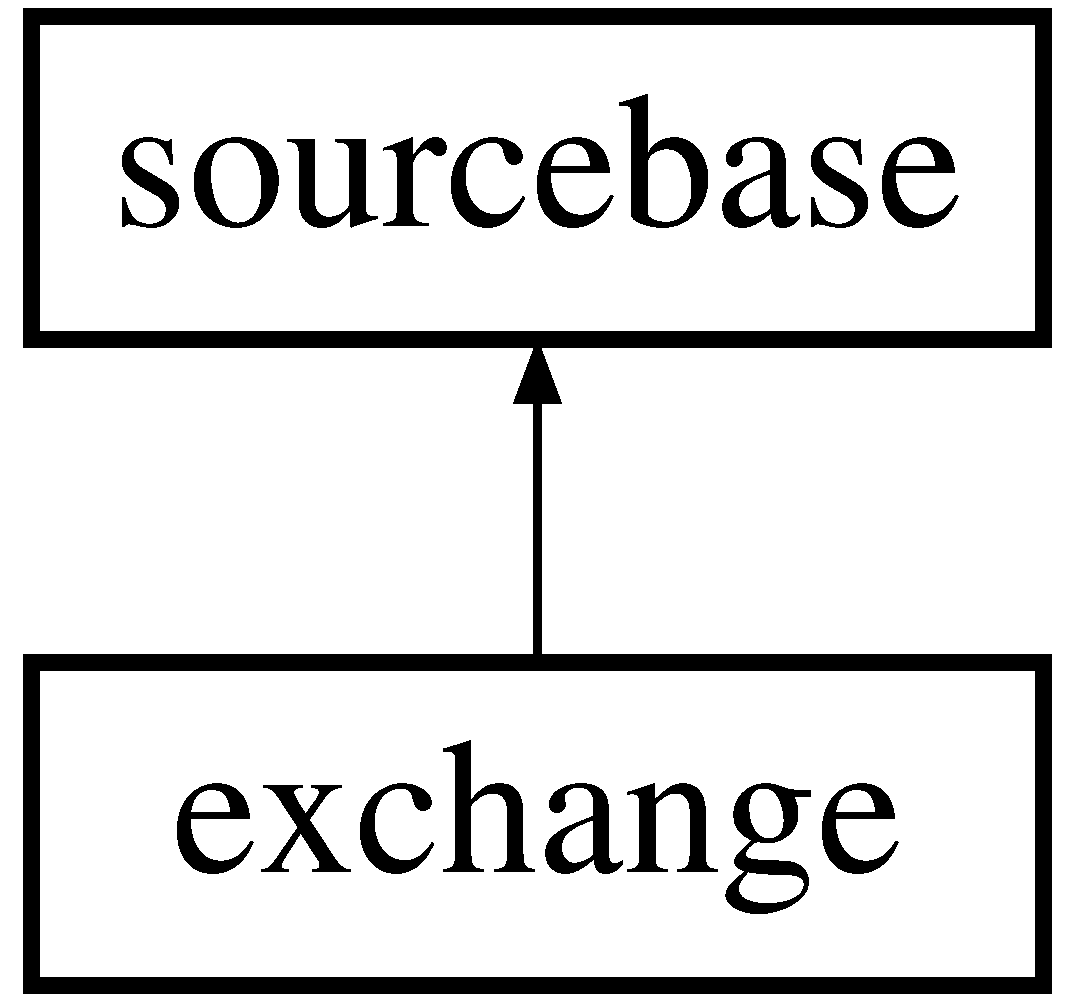
\includegraphics[height=2.000000cm]{classexchange}
\end{center}
\end{figure}
\subsection*{Public Member Functions}
\begin{DoxyCompactItemize}
\item 
void {\bf eval} (double $\ast$, double $\ast$, double $\ast$, double $\ast$)
\begin{DoxyCompactList}\small\item\em Evaluation of the Source in the Shallow Water Equations and Bed Sediment and Suspended Sediment Exchange. \end{DoxyCompactList}\end{DoxyCompactItemize}


\subsection{Detailed Description}
Derived Exchange Class from Source\-Base. 

\subsection{Member Function Documentation}
\index{exchange@{exchange}!eval@{eval}}
\index{eval@{eval}!exchange@{exchange}}
\subsubsection[{eval}]{\setlength{\rightskip}{0pt plus 5cm}void exchange\-::eval (
\begin{DoxyParamCaption}
\item[{double $\ast$}]{F2, }
\item[{double $\ast$}]{u\-L, }
\item[{double $\ast$}]{u\-Lslope, }
\item[{double $\ast$}]{q\-L}
\end{DoxyParamCaption}
)\hspace{0.3cm}{\ttfamily [virtual]}}\label{classexchange_a41c0e65e9f5c985db1672edf390b09e1}


Evaluation of the Source in the Shallow Water Equations and Bed Sediment and Suspended Sediment Exchange. 


\begin{DoxyItemize}
\item H\-\_\-0 / (U\-\_\-0)$^\wedge$2; 
\end{DoxyItemize}

Implements {\bf sourcebase} \doxyref{}{p.}{classsourcebase_aa47f29eea4fb554586279a5fa9394cb6}.



References Grass\-\_\-const, gravity\-\_\-const, and element\-::systemsize1.



The documentation for this class was generated from the following files\-:\begin{DoxyCompactItemize}
\item 
{\bf source.\-h}\item 
{\bf source.\-cpp}\end{DoxyCompactItemize}

\section{flux2base Class Reference}
\label{classflux2base}\index{flux2base@{flux2base}}


Local Dicontinuous Galerkin Flux Class.  




{\ttfamily \#include $<$flux2.\-h$>$}

Inheritance diagram for flux2base\-:\begin{figure}[H]
\begin{center}
\leavevmode
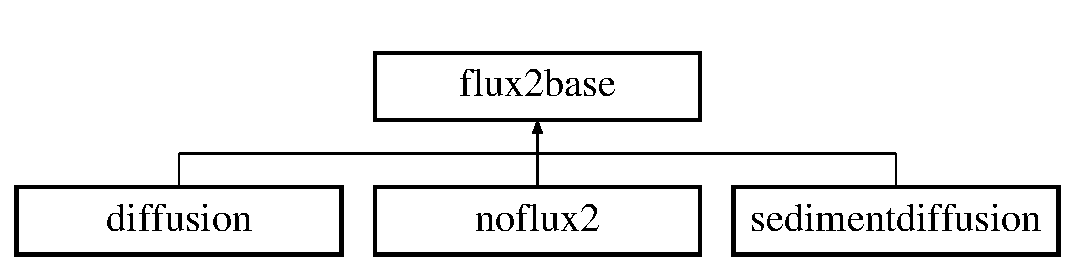
\includegraphics[height=2.000000cm]{classflux2base}
\end{center}
\end{figure}
\subsection*{Public Member Functions}
\begin{DoxyCompactItemize}
\item 
virtual double {\bf eval} (double $\ast$, double $\ast$, double $\ast$)=0
\begin{DoxyCompactList}\small\item\em Virtual Evaluation of the L\-D\-G flux. \end{DoxyCompactList}\end{DoxyCompactItemize}


\subsection{Detailed Description}
Local Dicontinuous Galerkin Flux Class. 

\subsection{Member Function Documentation}
\index{flux2base@{flux2base}!eval@{eval}}
\index{eval@{eval}!flux2base@{flux2base}}
\subsubsection[{eval}]{\setlength{\rightskip}{0pt plus 5cm}virtual double flux2base\-::eval (
\begin{DoxyParamCaption}
\item[{double $\ast$}]{, }
\item[{double $\ast$}]{, }
\item[{double $\ast$}]{}
\end{DoxyParamCaption}
)\hspace{0.3cm}{\ttfamily [pure virtual]}}\label{classflux2base_a4ecfc0d7470722ef299fa054c926f540}


Virtual Evaluation of the L\-D\-G flux. 



Implemented in {\bf sedimentdiffusion} \doxyref{}{p.}{classsedimentdiffusion_a99e5ded19d1a705b9eda6d0983de22ff}, {\bf diffusion} \doxyref{}{p.}{classdiffusion_a998c0963f4273bdb1b81e434501caf7e}, and {\bf noflux2} \doxyref{}{p.}{classnoflux2_ad26983eeb8b15565df7d2a3d3ec75daa}.



Referenced by flux2proc().



The documentation for this class was generated from the following file\-:\begin{DoxyCompactItemize}
\item 
{\bf flux2.\-h}\end{DoxyCompactItemize}

\section{fluxbase Class Reference}
\label{classfluxbase}\index{fluxbase@{fluxbase}}


Class Fluxbase.  




{\ttfamily \#include $<$flux.\-h$>$}

Inheritance diagram for fluxbase\-:\begin{figure}[H]
\begin{center}
\leavevmode
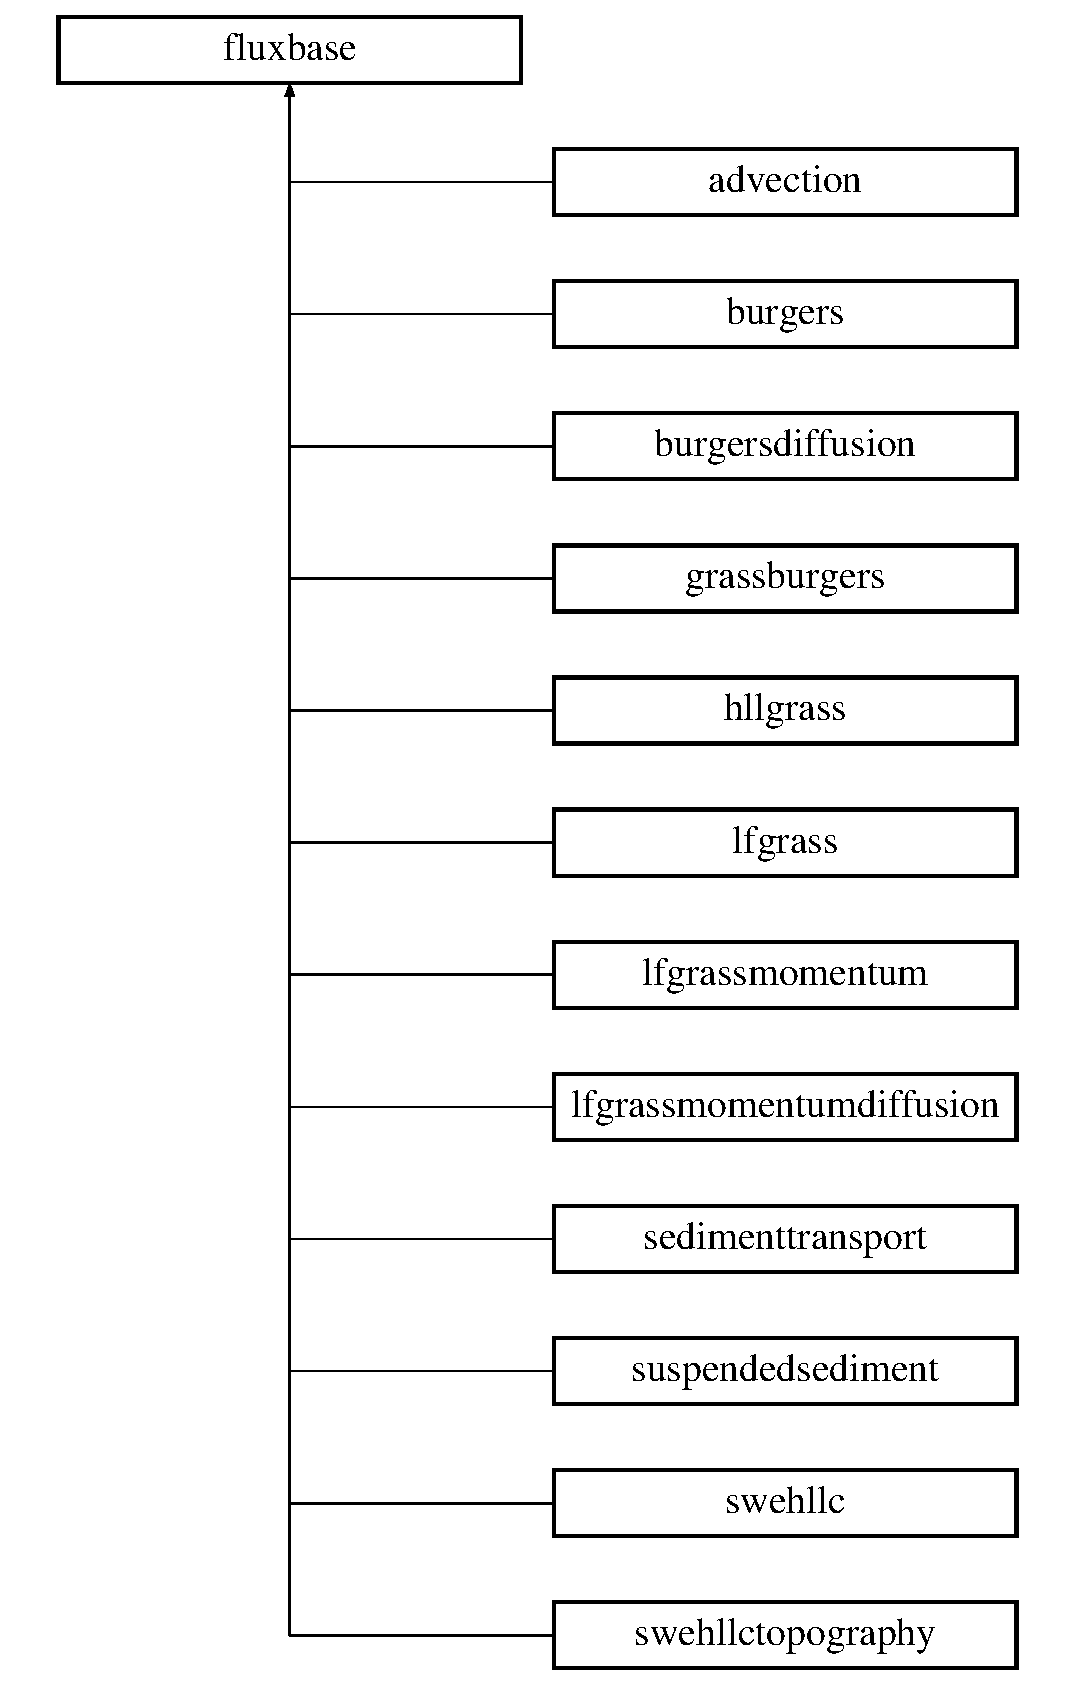
\includegraphics[height=12.000000cm]{classfluxbase}
\end{center}
\end{figure}
\subsection*{Public Member Functions}
\begin{DoxyCompactItemize}
\item 
virtual double {\bf eval} (double $\ast$, double $\ast$, double $\ast$, double $\ast$, double $\ast$)=0
\begin{DoxyCompactList}\small\item\em Virtual evaluation of the flux. \end{DoxyCompactList}\item 
virtual void {\bf eval\-\_\-l} (double $\ast$, double $\ast$, double $\ast$, double $\ast$, double $\ast$)=0
\begin{DoxyCompactList}\small\item\em Virtual non conservative evaluation of the flux on the left of the element. \end{DoxyCompactList}\item 
virtual void {\bf eval\-\_\-r} (double $\ast$, double $\ast$, double $\ast$, double $\ast$, double $\ast$)=0
\begin{DoxyCompactList}\small\item\em Virtual non conservative evaluation of the flux on the right of the element. \end{DoxyCompactList}\end{DoxyCompactItemize}


\subsection{Detailed Description}
Class Fluxbase. 

\subsection{Member Function Documentation}
\index{fluxbase@{fluxbase}!eval@{eval}}
\index{eval@{eval}!fluxbase@{fluxbase}}
\subsubsection[{eval}]{\setlength{\rightskip}{0pt plus 5cm}virtual double fluxbase\-::eval (
\begin{DoxyParamCaption}
\item[{double $\ast$}]{, }
\item[{double $\ast$}]{, }
\item[{double $\ast$}]{, }
\item[{double $\ast$}]{, }
\item[{double $\ast$}]{}
\end{DoxyParamCaption}
)\hspace{0.3cm}{\ttfamily [pure virtual]}}\label{classfluxbase_ab41e8752c750488dbcbc8ef24e277110}


Virtual evaluation of the flux. 



Implemented in {\bf lfgrassmomentumdiffusion} \doxyref{}{p.}{classlfgrassmomentumdiffusion_af85373170c01bfb07746514e007e7ab6}, {\bf suspendedsediment} \doxyref{}{p.}{classsuspendedsediment_a26e0411516045d46bc504acc7407797e}, {\bf grassburgers} \doxyref{}{p.}{classgrassburgers_ae2753add9bf6283ee9109535b2ae9bc3}, {\bf lfgrassmomentum} \doxyref{}{p.}{classlfgrassmomentum_a250fc27c64ad8cd33ba8f5b63d83e835}, {\bf lfgrass} \doxyref{}{p.}{classlfgrass_a7f1e440a01f3df687c94afe761751ded}, {\bf hllgrass} \doxyref{}{p.}{classhllgrass_a77f4e0b84a110faf3cd1f5b68a5e9a3c}, {\bf sedimenttransport} \doxyref{}{p.}{classsedimenttransport_a05b589c655e8dd393a49acd530bf1e4f}, {\bf swehllctopography} \doxyref{}{p.}{classswehllctopography_a94451a4ed6ec36f3c79ef8145cc81d47}, {\bf swehllc} \doxyref{}{p.}{classswehllc_a3cdffa7499fb936220d0084343401cad}, {\bf burgersdiffusion} \doxyref{}{p.}{classburgersdiffusion_abb97ec0449cd1c0a8ad476b7de3a62a9}, {\bf burgers} \doxyref{}{p.}{classburgers_a0f757dbcb4dc096dc7d44a32b0a7a7df}, and {\bf advection} \doxyref{}{p.}{classadvection_a39ffeff22d8c4bab9b209305e9c2ff05}.



Referenced by fluxproc().

\index{fluxbase@{fluxbase}!eval\-\_\-l@{eval\-\_\-l}}
\index{eval\-\_\-l@{eval\-\_\-l}!fluxbase@{fluxbase}}
\subsubsection[{eval\-\_\-l}]{\setlength{\rightskip}{0pt plus 5cm}virtual void fluxbase\-::eval\-\_\-l (
\begin{DoxyParamCaption}
\item[{double $\ast$}]{, }
\item[{double $\ast$}]{, }
\item[{double $\ast$}]{, }
\item[{double $\ast$}]{, }
\item[{double $\ast$}]{}
\end{DoxyParamCaption}
)\hspace{0.3cm}{\ttfamily [pure virtual]}}\label{classfluxbase_a184e5d5629191871c6dd9cd6b4e82799}


Virtual non conservative evaluation of the flux on the left of the element. 



Implemented in {\bf lfgrassmomentumdiffusion} \doxyref{}{p.}{classlfgrassmomentumdiffusion_a536d62fbd5be494414d061b44ec6c92e}, {\bf suspendedsediment} \doxyref{}{p.}{classsuspendedsediment_af4d3a3daf5a292a36b438512704d4098}, {\bf grassburgers} \doxyref{}{p.}{classgrassburgers_ade85dba58662fb903843ea6005576acd}, {\bf lfgrassmomentum} \doxyref{}{p.}{classlfgrassmomentum_ac0c120c7646e0b92c9907f87f69bc7a3}, {\bf lfgrass} \doxyref{}{p.}{classlfgrass_a6b3a5ec337a60dc98cf6d1f002836f2f}, {\bf hllgrass} \doxyref{}{p.}{classhllgrass_a86ef7d244e018c6a4f64324e2bb70fc4}, {\bf sedimenttransport} \doxyref{}{p.}{classsedimenttransport_a3624de092117d19e1b355493a4059edb}, {\bf swehllctopography} \doxyref{}{p.}{classswehllctopography_a29fe7da27580e800cebbfb98f2646fc3}, {\bf swehllc} \doxyref{}{p.}{classswehllc_abaf31947a1472a531131f2569919a300}, {\bf burgersdiffusion} \doxyref{}{p.}{classburgersdiffusion_a0ba7b3bc143ecd0cfb40431f957dc552}, {\bf burgers} \doxyref{}{p.}{classburgers_ad2ecdd94d31dd2bbf4accdde9967e25e}, and {\bf advection} \doxyref{}{p.}{classadvection_a64544ecc593a0e2d9e53c80cddce46fd}.



Referenced by fluxproc().

\index{fluxbase@{fluxbase}!eval\-\_\-r@{eval\-\_\-r}}
\index{eval\-\_\-r@{eval\-\_\-r}!fluxbase@{fluxbase}}
\subsubsection[{eval\-\_\-r}]{\setlength{\rightskip}{0pt plus 5cm}virtual void fluxbase\-::eval\-\_\-r (
\begin{DoxyParamCaption}
\item[{double $\ast$}]{, }
\item[{double $\ast$}]{, }
\item[{double $\ast$}]{, }
\item[{double $\ast$}]{, }
\item[{double $\ast$}]{}
\end{DoxyParamCaption}
)\hspace{0.3cm}{\ttfamily [pure virtual]}}\label{classfluxbase_ab5e6afaa22aff4a1bbbce0bba561fed3}


Virtual non conservative evaluation of the flux on the right of the element. 



Implemented in {\bf lfgrassmomentumdiffusion} \doxyref{}{p.}{classlfgrassmomentumdiffusion_a93abb9587da0e5c8c2eee205e4f7e9cb}, {\bf suspendedsediment} \doxyref{}{p.}{classsuspendedsediment_a232c9be4aad28973ade9e46222489035}, {\bf grassburgers} \doxyref{}{p.}{classgrassburgers_ad41c129b038579f72dd5817673fdb577}, {\bf lfgrassmomentum} \doxyref{}{p.}{classlfgrassmomentum_affb49cf7a846c68281f955a36ba4d40a}, {\bf lfgrass} \doxyref{}{p.}{classlfgrass_a8b0de0a21d4c2d5782fb335ba83a08fd}, {\bf hllgrass} \doxyref{}{p.}{classhllgrass_a779c9570d1ed6cf821cb4a3f18287019}, {\bf sedimenttransport} \doxyref{}{p.}{classsedimenttransport_a5d1143b0cfff17016fd5eb2acb9fc1b8}, {\bf swehllctopography} \doxyref{}{p.}{classswehllctopography_a858997ee906ad37ec1490abaff502841}, {\bf swehllc} \doxyref{}{p.}{classswehllc_af72fc457d5445284b1cef0cdd28071af}, {\bf burgersdiffusion} \doxyref{}{p.}{classburgersdiffusion_aa369a3cc470f23bb10b9415efb27b677}, {\bf burgers} \doxyref{}{p.}{classburgers_ae0a45d14818eed9d9df8236e6bf6e2b0}, and {\bf advection} \doxyref{}{p.}{classadvection_a17852fcad013696082568c732fe89003}.



Referenced by fluxproc().



The documentation for this class was generated from the following file\-:\begin{DoxyCompactItemize}
\item 
{\bf flux.\-h}\end{DoxyCompactItemize}

\section{grassburgers Class Reference}
\label{classgrassburgers}\index{grassburgers@{grassburgers}}


{\ttfamily \#include $<$flux.\-h$>$}

Inheritance diagram for grassburgers\-:\begin{figure}[H]
\begin{center}
\leavevmode
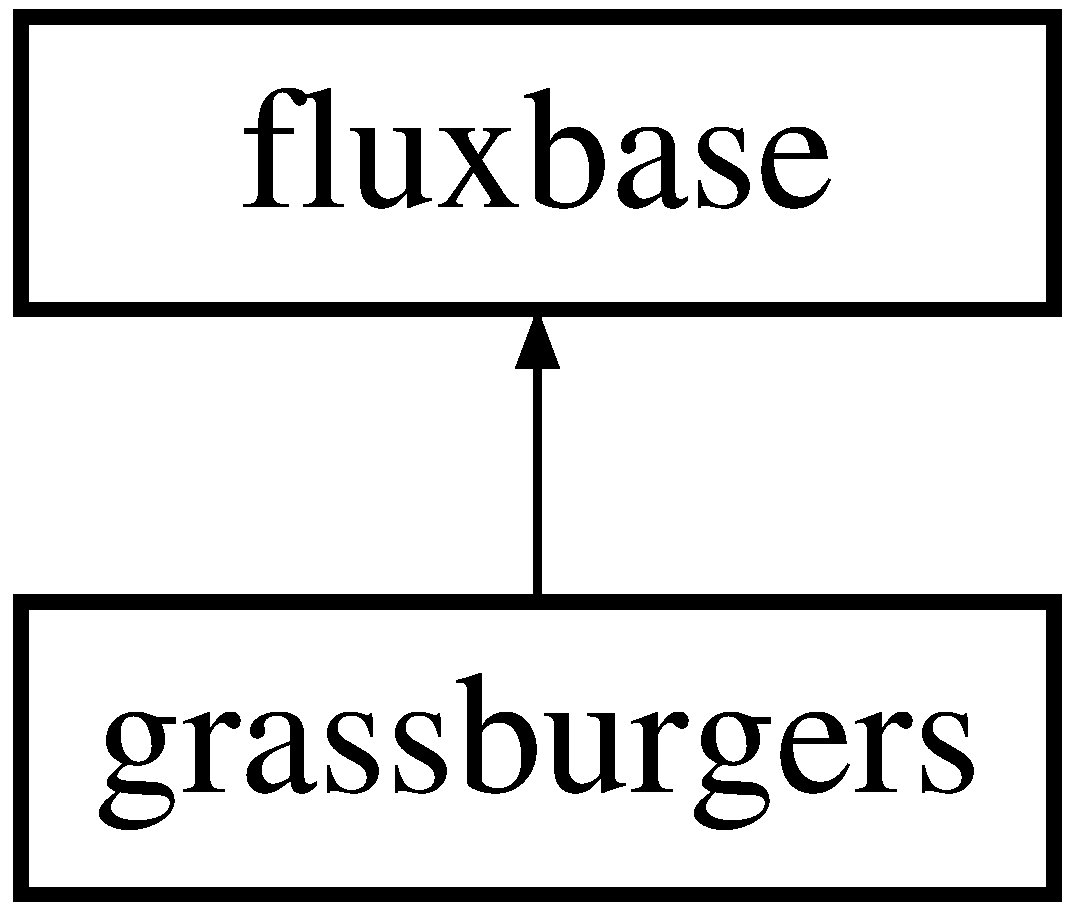
\includegraphics[height=2.000000cm]{classgrassburgers}
\end{center}
\end{figure}
\subsection*{Public Member Functions}
\begin{DoxyCompactItemize}
\item 
double {\bf eval} (double $\ast$, double $\ast$, double $\ast$, double $\ast$, double $\ast$)
\begin{DoxyCompactList}\small\item\em Evaluation of the assymtotic Grass bed updating equation as a sort of burgers equation. \end{DoxyCompactList}\item 
void {\bf eval\-\_\-l} (double $\ast$, double $\ast$, double $\ast$, double $\ast$, double $\ast$)
\begin{DoxyCompactList}\small\item\em Virtual non conservative evaluation of the flux on the left of the element. \end{DoxyCompactList}\item 
void {\bf eval\-\_\-r} (double $\ast$, double $\ast$, double $\ast$, double $\ast$, double $\ast$)
\begin{DoxyCompactList}\small\item\em Virtual non conservative evaluation of the flux on the right of the element. \end{DoxyCompactList}\end{DoxyCompactItemize}


\subsection{Member Function Documentation}
\index{grassburgers@{grassburgers}!eval@{eval}}
\index{eval@{eval}!grassburgers@{grassburgers}}
\subsubsection[{eval}]{\setlength{\rightskip}{0pt plus 5cm}double grassburgers\-::eval (
\begin{DoxyParamCaption}
\item[{double $\ast$}]{F, }
\item[{double $\ast$}]{u\-L, }
\item[{double $\ast$}]{u\-R, }
\item[{double $\ast$}]{q\-L, }
\item[{double $\ast$}]{q\-R}
\end{DoxyParamCaption}
)\hspace{0.3cm}{\ttfamily [virtual]}}\label{classgrassburgers_ae2753add9bf6283ee9109535b2ae9bc3}


Evaluation of the assymtotic Grass bed updating equation as a sort of burgers equation. 



Implements {\bf fluxbase} \doxyref{}{p.}{classfluxbase_ab41e8752c750488dbcbc8ef24e277110}.



References Grass\-\_\-const, Grass\-\_\-exponent, and element\-::systemsize1.

\index{grassburgers@{grassburgers}!eval\-\_\-l@{eval\-\_\-l}}
\index{eval\-\_\-l@{eval\-\_\-l}!grassburgers@{grassburgers}}
\subsubsection[{eval\-\_\-l}]{\setlength{\rightskip}{0pt plus 5cm}void grassburgers\-::eval\-\_\-l (
\begin{DoxyParamCaption}
\item[{double $\ast$}]{, }
\item[{double $\ast$}]{, }
\item[{double $\ast$}]{, }
\item[{double $\ast$}]{, }
\item[{double $\ast$}]{}
\end{DoxyParamCaption}
)\hspace{0.3cm}{\ttfamily [inline]}, {\ttfamily [virtual]}}\label{classgrassburgers_ade85dba58662fb903843ea6005576acd}


Virtual non conservative evaluation of the flux on the left of the element. 



Implements {\bf fluxbase} \doxyref{}{p.}{classfluxbase_a184e5d5629191871c6dd9cd6b4e82799}.

\index{grassburgers@{grassburgers}!eval\-\_\-r@{eval\-\_\-r}}
\index{eval\-\_\-r@{eval\-\_\-r}!grassburgers@{grassburgers}}
\subsubsection[{eval\-\_\-r}]{\setlength{\rightskip}{0pt plus 5cm}void grassburgers\-::eval\-\_\-r (
\begin{DoxyParamCaption}
\item[{double $\ast$}]{, }
\item[{double $\ast$}]{, }
\item[{double $\ast$}]{, }
\item[{double $\ast$}]{, }
\item[{double $\ast$}]{}
\end{DoxyParamCaption}
)\hspace{0.3cm}{\ttfamily [inline]}, {\ttfamily [virtual]}}\label{classgrassburgers_ad41c129b038579f72dd5817673fdb577}


Virtual non conservative evaluation of the flux on the right of the element. 



Implements {\bf fluxbase} \doxyref{}{p.}{classfluxbase_ab5e6afaa22aff4a1bbbce0bba561fed3}.



The documentation for this class was generated from the following files\-:\begin{DoxyCompactItemize}
\item 
{\bf flux.\-h}\item 
{\bf flux.\-cpp}\end{DoxyCompactItemize}

\section{hllgrass Class Reference}
\label{classhllgrass}\index{hllgrass@{hllgrass}}


Derived fluxbase class for assymtotic formulation of the Shallow Water equations including Grass' Bed Updating Equation using H\-L\-L.  




{\ttfamily \#include $<$flux.\-h$>$}

Inheritance diagram for hllgrass\-:\begin{figure}[H]
\begin{center}
\leavevmode
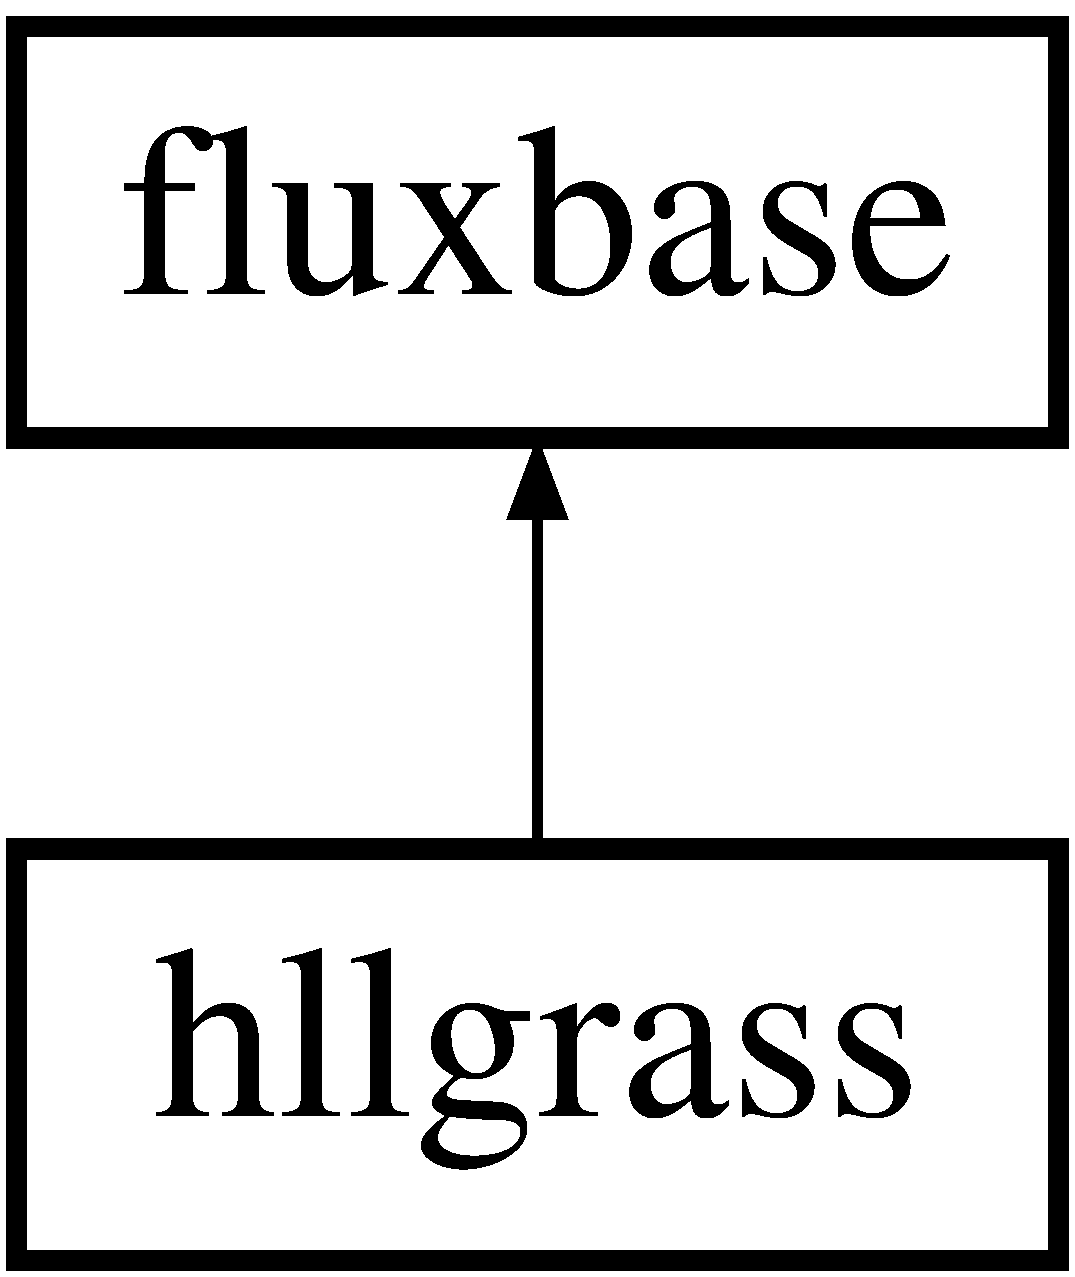
\includegraphics[height=2.000000cm]{classhllgrass}
\end{center}
\end{figure}
\subsection*{Public Member Functions}
\begin{DoxyCompactItemize}
\item 
double {\bf eval} (double $\ast$, double $\ast$, double $\ast$, double $\ast$, double $\ast$)
\begin{DoxyCompactList}\small\item\em Evaluation of the H\-L\-L flux. \end{DoxyCompactList}\item 
void {\bf eval\-\_\-l} (double $\ast$, double $\ast$, double $\ast$, double $\ast$, double $\ast$)
\begin{DoxyCompactList}\small\item\em Virtual non conservative evaluation of the flux on the left of the element. \end{DoxyCompactList}\item 
void {\bf eval\-\_\-r} (double $\ast$, double $\ast$, double $\ast$, double $\ast$, double $\ast$)
\begin{DoxyCompactList}\small\item\em Virtual non conservative evaluation of the flux on the right of the element. \end{DoxyCompactList}\end{DoxyCompactItemize}


\subsection{Detailed Description}
Derived fluxbase class for assymtotic formulation of the Shallow Water equations including Grass' Bed Updating Equation using H\-L\-L. 

\subsection{Member Function Documentation}
\index{hllgrass@{hllgrass}!eval@{eval}}
\index{eval@{eval}!hllgrass@{hllgrass}}
\subsubsection[{eval}]{\setlength{\rightskip}{0pt plus 5cm}double hllgrass\-::eval (
\begin{DoxyParamCaption}
\item[{double $\ast$}]{F, }
\item[{double $\ast$}]{u\-L, }
\item[{double $\ast$}]{u\-R, }
\item[{double $\ast$}]{q\-L, }
\item[{double $\ast$}]{q\-R}
\end{DoxyParamCaption}
)\hspace{0.3cm}{\ttfamily [virtual]}}\label{classhllgrass_a77f4e0b84a110faf3cd1f5b68a5e9a3c}


Evaluation of the H\-L\-L flux. 



Implements {\bf fluxbase} \doxyref{}{p.}{classfluxbase_ab41e8752c750488dbcbc8ef24e277110}.



References Grass\-\_\-const, Grass\-\_\-exponent, and gravity\-\_\-const.

\index{hllgrass@{hllgrass}!eval\-\_\-l@{eval\-\_\-l}}
\index{eval\-\_\-l@{eval\-\_\-l}!hllgrass@{hllgrass}}
\subsubsection[{eval\-\_\-l}]{\setlength{\rightskip}{0pt plus 5cm}void hllgrass\-::eval\-\_\-l (
\begin{DoxyParamCaption}
\item[{double $\ast$}]{, }
\item[{double $\ast$}]{, }
\item[{double $\ast$}]{, }
\item[{double $\ast$}]{, }
\item[{double $\ast$}]{}
\end{DoxyParamCaption}
)\hspace{0.3cm}{\ttfamily [inline]}, {\ttfamily [virtual]}}\label{classhllgrass_a86ef7d244e018c6a4f64324e2bb70fc4}


Virtual non conservative evaluation of the flux on the left of the element. 



Implements {\bf fluxbase} \doxyref{}{p.}{classfluxbase_a184e5d5629191871c6dd9cd6b4e82799}.

\index{hllgrass@{hllgrass}!eval\-\_\-r@{eval\-\_\-r}}
\index{eval\-\_\-r@{eval\-\_\-r}!hllgrass@{hllgrass}}
\subsubsection[{eval\-\_\-r}]{\setlength{\rightskip}{0pt plus 5cm}void hllgrass\-::eval\-\_\-r (
\begin{DoxyParamCaption}
\item[{double $\ast$}]{, }
\item[{double $\ast$}]{, }
\item[{double $\ast$}]{, }
\item[{double $\ast$}]{, }
\item[{double $\ast$}]{}
\end{DoxyParamCaption}
)\hspace{0.3cm}{\ttfamily [inline]}, {\ttfamily [virtual]}}\label{classhllgrass_a779c9570d1ed6cf821cb4a3f18287019}


Virtual non conservative evaluation of the flux on the right of the element. 



Implements {\bf fluxbase} \doxyref{}{p.}{classfluxbase_ab5e6afaa22aff4a1bbbce0bba561fed3}.



The documentation for this class was generated from the following files\-:\begin{DoxyCompactItemize}
\item 
{\bf flux.\-h}\item 
{\bf flux.\-cpp}\end{DoxyCompactItemize}

\section{lfgrass Class Reference}
\label{classlfgrass}\index{lfgrass@{lfgrass}}


Derived fluxbase class for assymtotic formulation of the Shallow Water equations including Grass' Bed Updating Equation using L\-F.  




{\ttfamily \#include $<$flux.\-h$>$}

Inheritance diagram for lfgrass\-:\begin{figure}[H]
\begin{center}
\leavevmode
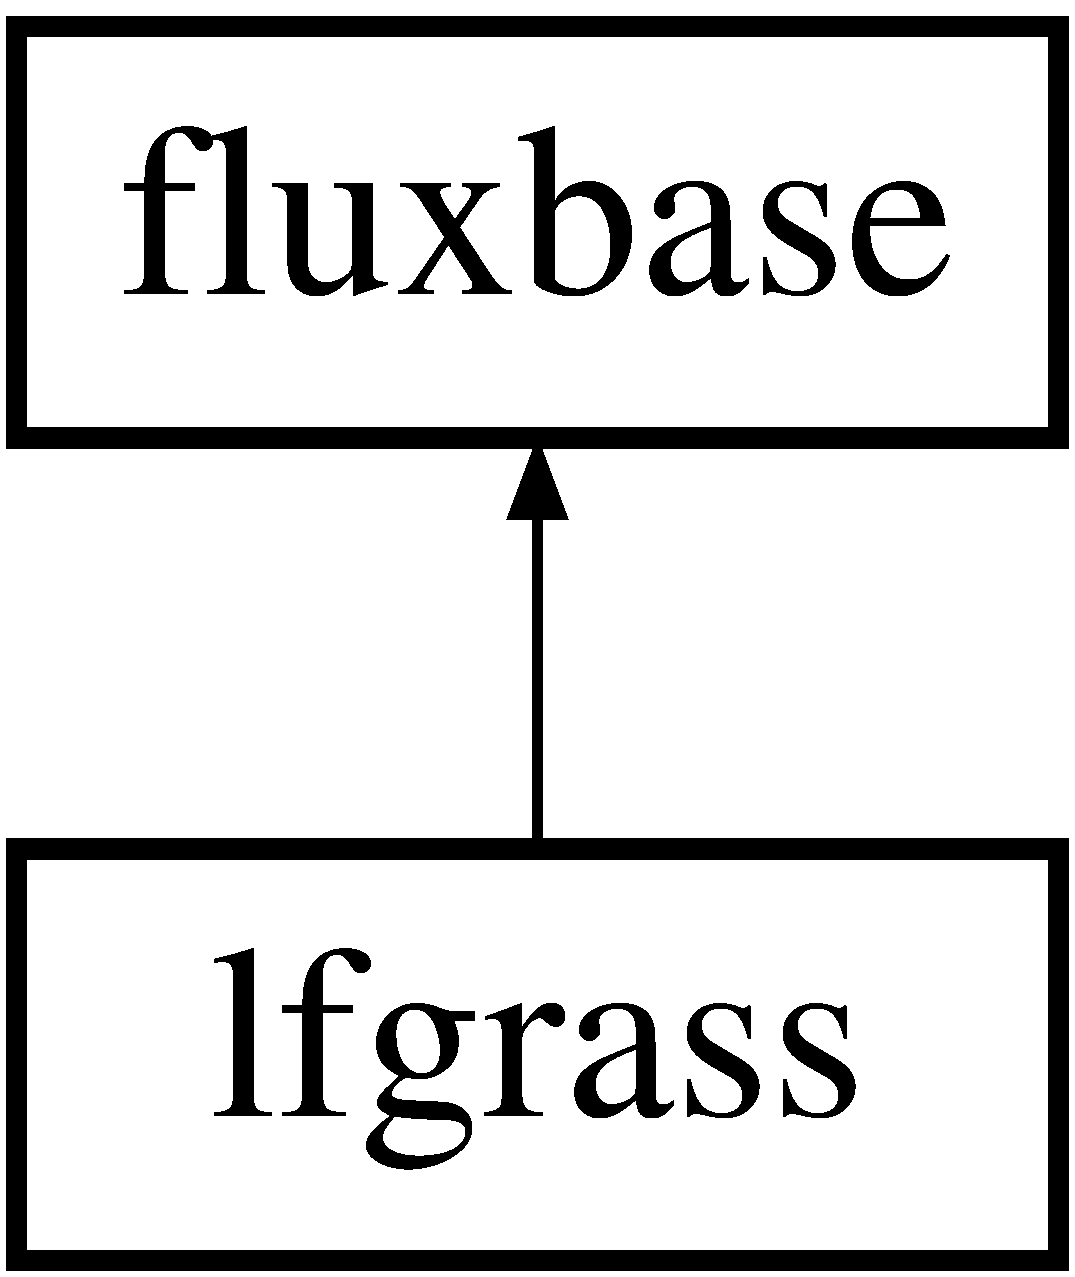
\includegraphics[height=2.000000cm]{classlfgrass}
\end{center}
\end{figure}
\subsection*{Public Member Functions}
\begin{DoxyCompactItemize}
\item 
double {\bf eval} (double $\ast$, double $\ast$, double $\ast$, double $\ast$, double $\ast$)
\begin{DoxyCompactList}\small\item\em Evaluation of the Lax Friedrichs flux. \end{DoxyCompactList}\item 
void {\bf eval\-\_\-l} (double $\ast$, double $\ast$, double $\ast$, double $\ast$, double $\ast$)
\begin{DoxyCompactList}\small\item\em Virtual non conservative evaluation of the flux on the left of the element. \end{DoxyCompactList}\item 
void {\bf eval\-\_\-r} (double $\ast$, double $\ast$, double $\ast$, double $\ast$, double $\ast$)
\begin{DoxyCompactList}\small\item\em Virtual non conservative evaluation of the flux on the right of the element. \end{DoxyCompactList}\end{DoxyCompactItemize}


\subsection{Detailed Description}
Derived fluxbase class for assymtotic formulation of the Shallow Water equations including Grass' Bed Updating Equation using L\-F. 

\subsection{Member Function Documentation}
\index{lfgrass@{lfgrass}!eval@{eval}}
\index{eval@{eval}!lfgrass@{lfgrass}}
\subsubsection[{eval}]{\setlength{\rightskip}{0pt plus 5cm}double lfgrass\-::eval (
\begin{DoxyParamCaption}
\item[{double $\ast$}]{F, }
\item[{double $\ast$}]{u\-L, }
\item[{double $\ast$}]{u\-R, }
\item[{double $\ast$}]{q\-L, }
\item[{double $\ast$}]{q\-R}
\end{DoxyParamCaption}
)\hspace{0.3cm}{\ttfamily [virtual]}}\label{classlfgrass_a7f1e440a01f3df687c94afe761751ded}


Evaluation of the Lax Friedrichs flux. 



Implements {\bf fluxbase} \doxyref{}{p.}{classfluxbase_ab41e8752c750488dbcbc8ef24e277110}.



References Grass\-\_\-const, Grass\-\_\-exponent, and gravity\-\_\-const.

\index{lfgrass@{lfgrass}!eval\-\_\-l@{eval\-\_\-l}}
\index{eval\-\_\-l@{eval\-\_\-l}!lfgrass@{lfgrass}}
\subsubsection[{eval\-\_\-l}]{\setlength{\rightskip}{0pt plus 5cm}void lfgrass\-::eval\-\_\-l (
\begin{DoxyParamCaption}
\item[{double $\ast$}]{, }
\item[{double $\ast$}]{, }
\item[{double $\ast$}]{, }
\item[{double $\ast$}]{, }
\item[{double $\ast$}]{}
\end{DoxyParamCaption}
)\hspace{0.3cm}{\ttfamily [inline]}, {\ttfamily [virtual]}}\label{classlfgrass_a6b3a5ec337a60dc98cf6d1f002836f2f}


Virtual non conservative evaluation of the flux on the left of the element. 



Implements {\bf fluxbase} \doxyref{}{p.}{classfluxbase_a184e5d5629191871c6dd9cd6b4e82799}.

\index{lfgrass@{lfgrass}!eval\-\_\-r@{eval\-\_\-r}}
\index{eval\-\_\-r@{eval\-\_\-r}!lfgrass@{lfgrass}}
\subsubsection[{eval\-\_\-r}]{\setlength{\rightskip}{0pt plus 5cm}void lfgrass\-::eval\-\_\-r (
\begin{DoxyParamCaption}
\item[{double $\ast$}]{, }
\item[{double $\ast$}]{, }
\item[{double $\ast$}]{, }
\item[{double $\ast$}]{, }
\item[{double $\ast$}]{}
\end{DoxyParamCaption}
)\hspace{0.3cm}{\ttfamily [inline]}, {\ttfamily [virtual]}}\label{classlfgrass_a8b0de0a21d4c2d5782fb335ba83a08fd}


Virtual non conservative evaluation of the flux on the right of the element. 



Implements {\bf fluxbase} \doxyref{}{p.}{classfluxbase_ab5e6afaa22aff4a1bbbce0bba561fed3}.



The documentation for this class was generated from the following files\-:\begin{DoxyCompactItemize}
\item 
{\bf flux.\-h}\item 
{\bf flux.\-cpp}\end{DoxyCompactItemize}

\section{lfgrassmomentum Class Reference}
\label{classlfgrassmomentum}\index{lfgrassmomentum@{lfgrassmomentum}}


Derived fluxbase class for the Shallow Water equations including Grass' Bed Updating Equation using L\-F.  




{\ttfamily \#include $<$flux.\-h$>$}

Inheritance diagram for lfgrassmomentum\-:\begin{figure}[H]
\begin{center}
\leavevmode
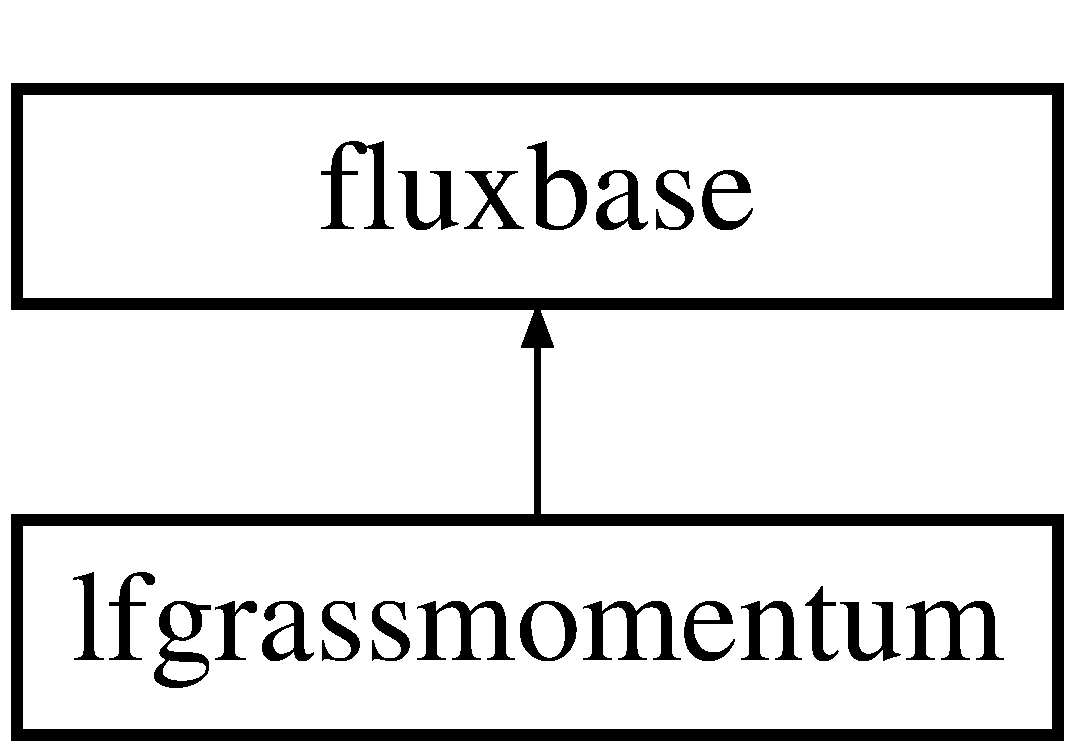
\includegraphics[height=2.000000cm]{classlfgrassmomentum}
\end{center}
\end{figure}
\subsection*{Public Member Functions}
\begin{DoxyCompactItemize}
\item 
double {\bf eval} (double $\ast$, double $\ast$, double $\ast$, double $\ast$, double $\ast$)
\begin{DoxyCompactList}\small\item\em Evaluation of the Lax Friedrichs flux with topography correction. \end{DoxyCompactList}\item 
void {\bf eval\-\_\-l} (double $\ast$, double $\ast$, double $\ast$, double $\ast$, double $\ast$)
\begin{DoxyCompactList}\small\item\em Non conservative flux as suggested by Bouchut et al. (2004). \end{DoxyCompactList}\item 
void {\bf eval\-\_\-r} (double $\ast$, double $\ast$, double $\ast$, double $\ast$, double $\ast$)
\begin{DoxyCompactList}\small\item\em Non conservative flux as suggested by Bouchut et al. (2004). \end{DoxyCompactList}\end{DoxyCompactItemize}


\subsection{Detailed Description}
Derived fluxbase class for the Shallow Water equations including Grass' Bed Updating Equation using L\-F. 

\subsection{Member Function Documentation}
\index{lfgrassmomentum@{lfgrassmomentum}!eval@{eval}}
\index{eval@{eval}!lfgrassmomentum@{lfgrassmomentum}}
\subsubsection[{eval}]{\setlength{\rightskip}{0pt plus 5cm}double lfgrassmomentum\-::eval (
\begin{DoxyParamCaption}
\item[{double $\ast$}]{F, }
\item[{double $\ast$}]{u\-L, }
\item[{double $\ast$}]{u\-R, }
\item[{double $\ast$}]{q\-L, }
\item[{double $\ast$}]{q\-R}
\end{DoxyParamCaption}
)\hspace{0.3cm}{\ttfamily [virtual]}}\label{classlfgrassmomentum_a250fc27c64ad8cd33ba8f5b63d83e835}


Evaluation of the Lax Friedrichs flux with topography correction. 



Implements {\bf fluxbase} \doxyref{}{p.}{classfluxbase_ab41e8752c750488dbcbc8ef24e277110}.



References Grass\-\_\-const, Grass\-\_\-exponent, and gravity\-\_\-const.

\index{lfgrassmomentum@{lfgrassmomentum}!eval\-\_\-l@{eval\-\_\-l}}
\index{eval\-\_\-l@{eval\-\_\-l}!lfgrassmomentum@{lfgrassmomentum}}
\subsubsection[{eval\-\_\-l}]{\setlength{\rightskip}{0pt plus 5cm}void lfgrassmomentum\-::eval\-\_\-l (
\begin{DoxyParamCaption}
\item[{double $\ast$}]{Fl, }
\item[{double $\ast$}]{u\-L, }
\item[{double $\ast$}]{u\-R, }
\item[{double $\ast$}]{q\-L, }
\item[{double $\ast$}]{q\-R}
\end{DoxyParamCaption}
)\hspace{0.3cm}{\ttfamily [virtual]}}\label{classlfgrassmomentum_ac0c120c7646e0b92c9907f87f69bc7a3}


Non conservative flux as suggested by Bouchut et al. (2004). 



Implements {\bf fluxbase} \doxyref{}{p.}{classfluxbase_a184e5d5629191871c6dd9cd6b4e82799}.



References gravity\-\_\-const, and element\-::systemsize1.

\index{lfgrassmomentum@{lfgrassmomentum}!eval\-\_\-r@{eval\-\_\-r}}
\index{eval\-\_\-r@{eval\-\_\-r}!lfgrassmomentum@{lfgrassmomentum}}
\subsubsection[{eval\-\_\-r}]{\setlength{\rightskip}{0pt plus 5cm}void lfgrassmomentum\-::eval\-\_\-r (
\begin{DoxyParamCaption}
\item[{double $\ast$}]{Fr, }
\item[{double $\ast$}]{u\-L, }
\item[{double $\ast$}]{u\-R, }
\item[{double $\ast$}]{q\-L, }
\item[{double $\ast$}]{q\-R}
\end{DoxyParamCaption}
)\hspace{0.3cm}{\ttfamily [virtual]}}\label{classlfgrassmomentum_affb49cf7a846c68281f955a36ba4d40a}


Non conservative flux as suggested by Bouchut et al. (2004). 



Implements {\bf fluxbase} \doxyref{}{p.}{classfluxbase_ab5e6afaa22aff4a1bbbce0bba561fed3}.



References gravity\-\_\-const, and element\-::systemsize1.



The documentation for this class was generated from the following files\-:\begin{DoxyCompactItemize}
\item 
{\bf flux.\-h}\item 
{\bf flux.\-cpp}\end{DoxyCompactItemize}

\section{lfgrassmomentumdiffusion Class Reference}
\label{classlfgrassmomentumdiffusion}\index{lfgrassmomentumdiffusion@{lfgrassmomentumdiffusion}}


Derived fluxbase class for the Shallow Water equations including Grass' Bed Updating Equation using L\-F and L\-D\-G for diffusion term.  




{\ttfamily \#include $<$flux.\-h$>$}

Inheritance diagram for lfgrassmomentumdiffusion\-:\begin{figure}[H]
\begin{center}
\leavevmode
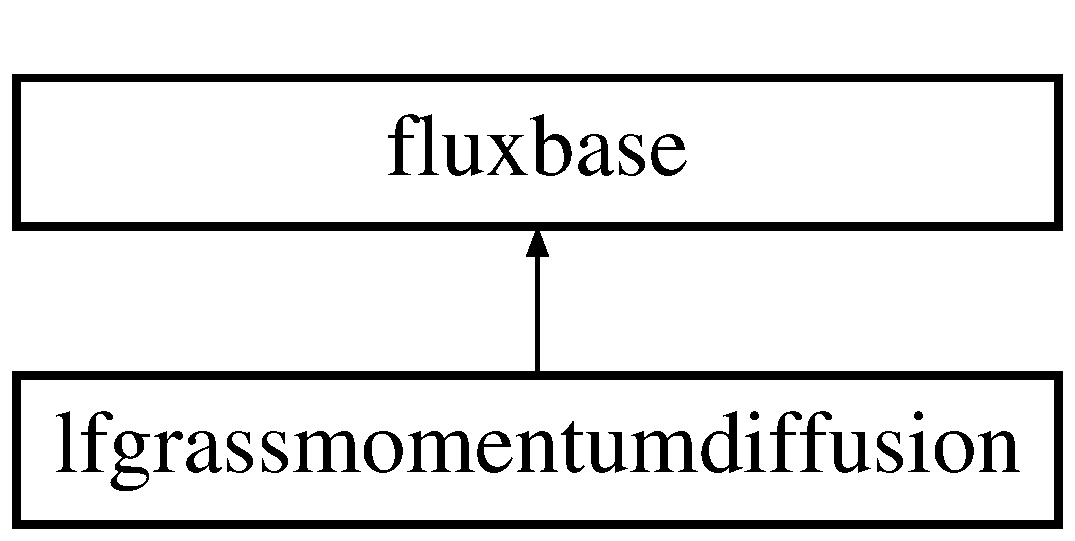
\includegraphics[height=2.000000cm]{classlfgrassmomentumdiffusion}
\end{center}
\end{figure}
\subsection*{Public Member Functions}
\begin{DoxyCompactItemize}
\item 
double {\bf eval} (double $\ast$, double $\ast$, double $\ast$, double $\ast$, double $\ast$)
\begin{DoxyCompactList}\small\item\em Evaluation of the Lax Friedrichs flux with topography correction. \end{DoxyCompactList}\item 
void {\bf eval\-\_\-l} (double $\ast$, double $\ast$, double $\ast$, double $\ast$, double $\ast$)
\begin{DoxyCompactList}\small\item\em Non conservative flux as suggested by Bouchut et al. (2004). \end{DoxyCompactList}\item 
void {\bf eval\-\_\-r} (double $\ast$, double $\ast$, double $\ast$, double $\ast$, double $\ast$)
\begin{DoxyCompactList}\small\item\em Non conservative flux as suggested by Bouchut et al. (2004). \end{DoxyCompactList}\end{DoxyCompactItemize}


\subsection{Detailed Description}
Derived fluxbase class for the Shallow Water equations including Grass' Bed Updating Equation using L\-F and L\-D\-G for diffusion term. 

\subsection{Member Function Documentation}
\index{lfgrassmomentumdiffusion@{lfgrassmomentumdiffusion}!eval@{eval}}
\index{eval@{eval}!lfgrassmomentumdiffusion@{lfgrassmomentumdiffusion}}
\subsubsection[{eval}]{\setlength{\rightskip}{0pt plus 5cm}double lfgrassmomentumdiffusion\-::eval (
\begin{DoxyParamCaption}
\item[{double $\ast$}]{F, }
\item[{double $\ast$}]{u\-L, }
\item[{double $\ast$}]{u\-R, }
\item[{double $\ast$}]{q\-L, }
\item[{double $\ast$}]{q\-R}
\end{DoxyParamCaption}
)\hspace{0.3cm}{\ttfamily [virtual]}}\label{classlfgrassmomentumdiffusion_af85373170c01bfb07746514e007e7ab6}


Evaluation of the Lax Friedrichs flux with topography correction. 



Implements {\bf fluxbase} \doxyref{}{p.}{classfluxbase_ab41e8752c750488dbcbc8ef24e277110}.



References Grass\-\_\-const, Grass\-\_\-exponent, and gravity\-\_\-const.

\index{lfgrassmomentumdiffusion@{lfgrassmomentumdiffusion}!eval\-\_\-l@{eval\-\_\-l}}
\index{eval\-\_\-l@{eval\-\_\-l}!lfgrassmomentumdiffusion@{lfgrassmomentumdiffusion}}
\subsubsection[{eval\-\_\-l}]{\setlength{\rightskip}{0pt plus 5cm}void lfgrassmomentumdiffusion\-::eval\-\_\-l (
\begin{DoxyParamCaption}
\item[{double $\ast$}]{Fl, }
\item[{double $\ast$}]{u\-L, }
\item[{double $\ast$}]{u\-R, }
\item[{double $\ast$}]{q\-L, }
\item[{double $\ast$}]{q\-R}
\end{DoxyParamCaption}
)\hspace{0.3cm}{\ttfamily [virtual]}}\label{classlfgrassmomentumdiffusion_a536d62fbd5be494414d061b44ec6c92e}


Non conservative flux as suggested by Bouchut et al. (2004). 



Implements {\bf fluxbase} \doxyref{}{p.}{classfluxbase_a184e5d5629191871c6dd9cd6b4e82799}.



References gravity\-\_\-const, and element\-::systemsize1.

\index{lfgrassmomentumdiffusion@{lfgrassmomentumdiffusion}!eval\-\_\-r@{eval\-\_\-r}}
\index{eval\-\_\-r@{eval\-\_\-r}!lfgrassmomentumdiffusion@{lfgrassmomentumdiffusion}}
\subsubsection[{eval\-\_\-r}]{\setlength{\rightskip}{0pt plus 5cm}void lfgrassmomentumdiffusion\-::eval\-\_\-r (
\begin{DoxyParamCaption}
\item[{double $\ast$}]{Fr, }
\item[{double $\ast$}]{u\-L, }
\item[{double $\ast$}]{u\-R, }
\item[{double $\ast$}]{q\-L, }
\item[{double $\ast$}]{q\-R}
\end{DoxyParamCaption}
)\hspace{0.3cm}{\ttfamily [virtual]}}\label{classlfgrassmomentumdiffusion_a93abb9587da0e5c8c2eee205e4f7e9cb}


Non conservative flux as suggested by Bouchut et al. (2004). 



Implements {\bf fluxbase} \doxyref{}{p.}{classfluxbase_ab5e6afaa22aff4a1bbbce0bba561fed3}.



References gravity\-\_\-const, and element\-::systemsize1.



The documentation for this class was generated from the following files\-:\begin{DoxyCompactItemize}
\item 
{\bf flux.\-h}\item 
{\bf flux.\-cpp}\end{DoxyCompactItemize}

\section{node Class Reference}
\label{classnode}\index{node@{node}}


Node Class (= Face)  




{\ttfamily \#include $<$node.\-h$>$}

\subsection*{Public Member Functions}
\begin{DoxyCompactItemize}
\item 
{\bf node} ()
\begin{DoxyCompactList}\small\item\em Default constructor\-: creates x;. \end{DoxyCompactList}\item 
{\bf node} (double)
\begin{DoxyCompactList}\small\item\em Overloading constructor assigning x = value;. \end{DoxyCompactList}\end{DoxyCompactItemize}
\subsection*{Public Attributes}
\begin{DoxyCompactItemize}
\item 
double {\bf x}
\begin{DoxyCompactList}\small\item\em x-\/value of the node. \end{DoxyCompactList}\item 
double $\ast$ {\bf u\-L}
\begin{DoxyCompactList}\small\item\em Value of system U on the left of the face. \end{DoxyCompactList}\item 
double $\ast$ {\bf u\-R}
\begin{DoxyCompactList}\small\item\em Value of system U on the right of the face. \end{DoxyCompactList}\item 
double $\ast$ {\bf q\-L}
\begin{DoxyCompactList}\small\item\em Value of system Q on the left of the face. \end{DoxyCompactList}\item 
double $\ast$ {\bf q\-R}
\begin{DoxyCompactList}\small\item\em Value of system Q on the right of the face. \end{DoxyCompactList}\end{DoxyCompactItemize}


\subsection{Detailed Description}
Node Class (= Face) 

\subsection{Constructor \& Destructor Documentation}
\index{node@{node}!node@{node}}
\index{node@{node}!node@{node}}
\subsubsection[{node}]{\setlength{\rightskip}{0pt plus 5cm}node\-::node (
\begin{DoxyParamCaption}
{}
\end{DoxyParamCaption}
)}\label{classnode_a82669b7358b50bd8d7888d7df4ff8dfa}


Default constructor\-: creates x;. 

\index{node@{node}!node@{node}}
\index{node@{node}!node@{node}}
\subsubsection[{node}]{\setlength{\rightskip}{0pt plus 5cm}node\-::node (
\begin{DoxyParamCaption}
\item[{double}]{value}
\end{DoxyParamCaption}
)}\label{classnode_af9adeba08694ce802ebd220127b14e33}


Overloading constructor assigning x = value;. 



References element\-::systemsize1, and element\-::systemsize2.



\subsection{Member Data Documentation}
\index{node@{node}!q\-L@{q\-L}}
\index{q\-L@{q\-L}!node@{node}}
\subsubsection[{q\-L}]{\setlength{\rightskip}{0pt plus 5cm}double$\ast$ node\-::q\-L}\label{classnode_a31faca1ebc6a7aebf35e853e2ad1dff9}


Value of system Q on the left of the face. 

\index{node@{node}!q\-R@{q\-R}}
\index{q\-R@{q\-R}!node@{node}}
\subsubsection[{q\-R}]{\setlength{\rightskip}{0pt plus 5cm}double$\ast$ node\-::q\-R}\label{classnode_ad013cb5981057c6350d713eec6628dce}


Value of system Q on the right of the face. 

\index{node@{node}!u\-L@{u\-L}}
\index{u\-L@{u\-L}!node@{node}}
\subsubsection[{u\-L}]{\setlength{\rightskip}{0pt plus 5cm}double$\ast$ node\-::u\-L}\label{classnode_a7599fcbb5f651ed36137ab87ed1a5a84}


Value of system U on the left of the face. 

\index{node@{node}!u\-R@{u\-R}}
\index{u\-R@{u\-R}!node@{node}}
\subsubsection[{u\-R}]{\setlength{\rightskip}{0pt plus 5cm}double$\ast$ node\-::u\-R}\label{classnode_a840c68dfb33d8f6ab1837863f1d017ef}


Value of system U on the right of the face. 

\index{node@{node}!x@{x}}
\index{x@{x}!node@{node}}
\subsubsection[{x}]{\setlength{\rightskip}{0pt plus 5cm}double node\-::x}\label{classnode_aabf3ca384568672adc30f70f01c9df10}


x-\/value of the node. 



The documentation for this class was generated from the following files\-:\begin{DoxyCompactItemize}
\item 
{\bf node.\-h}\item 
{\bf node.\-cpp}\end{DoxyCompactItemize}

\section{noflux2 Class Reference}
\label{classnoflux2}\index{noflux2@{noflux2}}


L\-D\-G noflux class Derived from \doxyref{flux2base}{p.}{classflux2base}.  




{\ttfamily \#include $<$flux2.\-h$>$}

Inheritance diagram for noflux2\-:\begin{figure}[H]
\begin{center}
\leavevmode
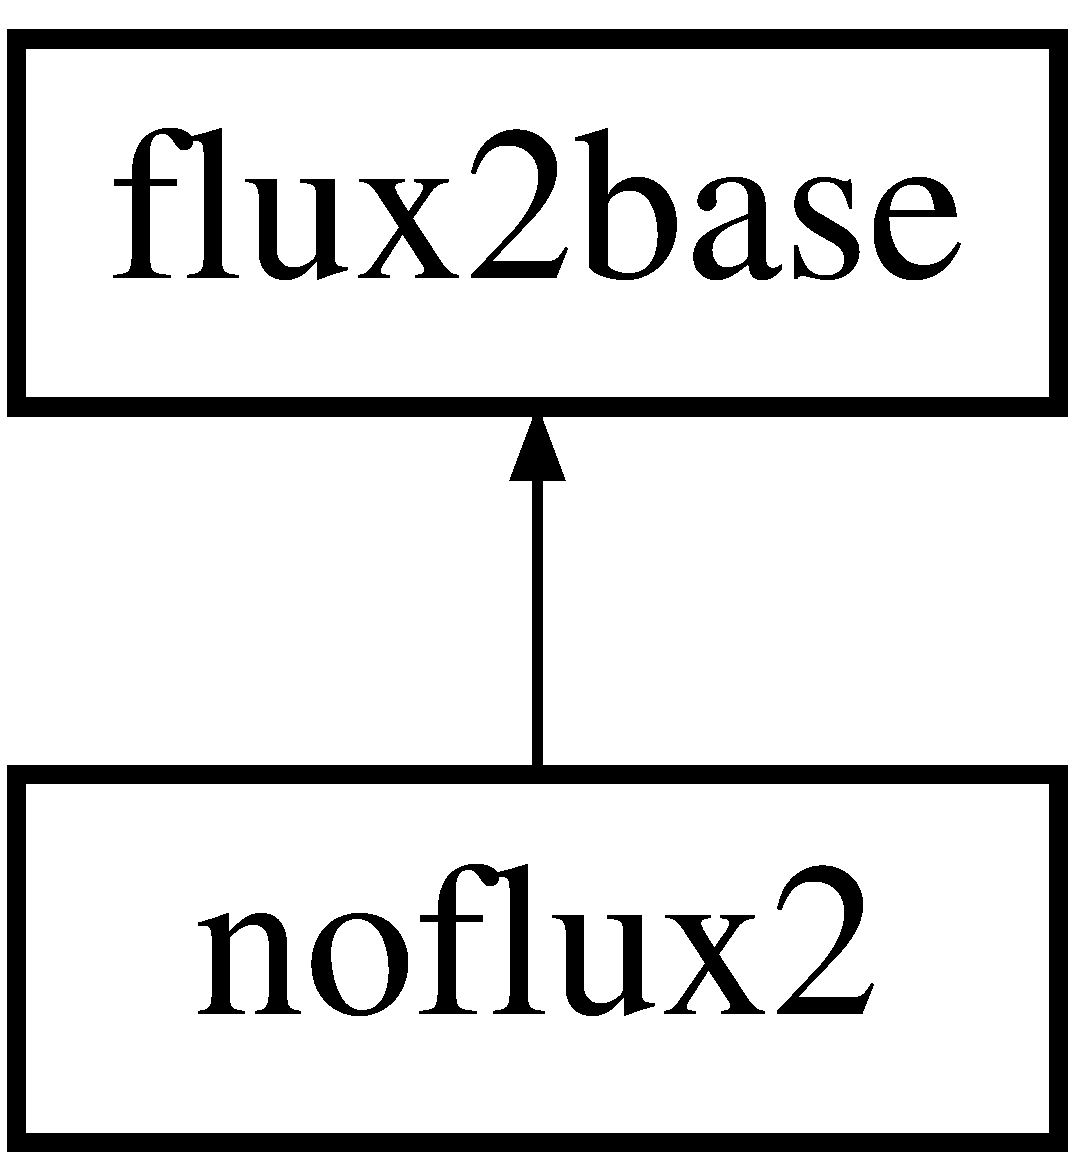
\includegraphics[height=2.000000cm]{classnoflux2}
\end{center}
\end{figure}
\subsection*{Public Member Functions}
\begin{DoxyCompactItemize}
\item 
double {\bf eval} (double $\ast$, double $\ast$, double $\ast$)
\begin{DoxyCompactList}\small\item\em Evaluation which does nothing. \end{DoxyCompactList}\end{DoxyCompactItemize}


\subsection{Detailed Description}
L\-D\-G noflux class Derived from \doxyref{flux2base}{p.}{classflux2base}. 

\subsection{Member Function Documentation}
\index{noflux2@{noflux2}!eval@{eval}}
\index{eval@{eval}!noflux2@{noflux2}}
\subsubsection[{eval}]{\setlength{\rightskip}{0pt plus 5cm}double noflux2\-::eval (
\begin{DoxyParamCaption}
\item[{double $\ast$}]{, }
\item[{double $\ast$}]{, }
\item[{double $\ast$}]{}
\end{DoxyParamCaption}
)\hspace{0.3cm}{\ttfamily [inline]}, {\ttfamily [virtual]}}\label{classnoflux2_ad26983eeb8b15565df7d2a3d3ec75daa}


Evaluation which does nothing. 



Implements {\bf flux2base} \doxyref{}{p.}{classflux2base_a4ecfc0d7470722ef299fa054c926f540}.



The documentation for this class was generated from the following file\-:\begin{DoxyCompactItemize}
\item 
{\bf flux2.\-h}\end{DoxyCompactItemize}

\section{nosource Class Reference}
\label{classnosource}\index{nosource@{nosource}}


Derived No\-Source Class from Source\-Base.  




{\ttfamily \#include $<$source.\-h$>$}

Inheritance diagram for nosource\-:\begin{figure}[H]
\begin{center}
\leavevmode
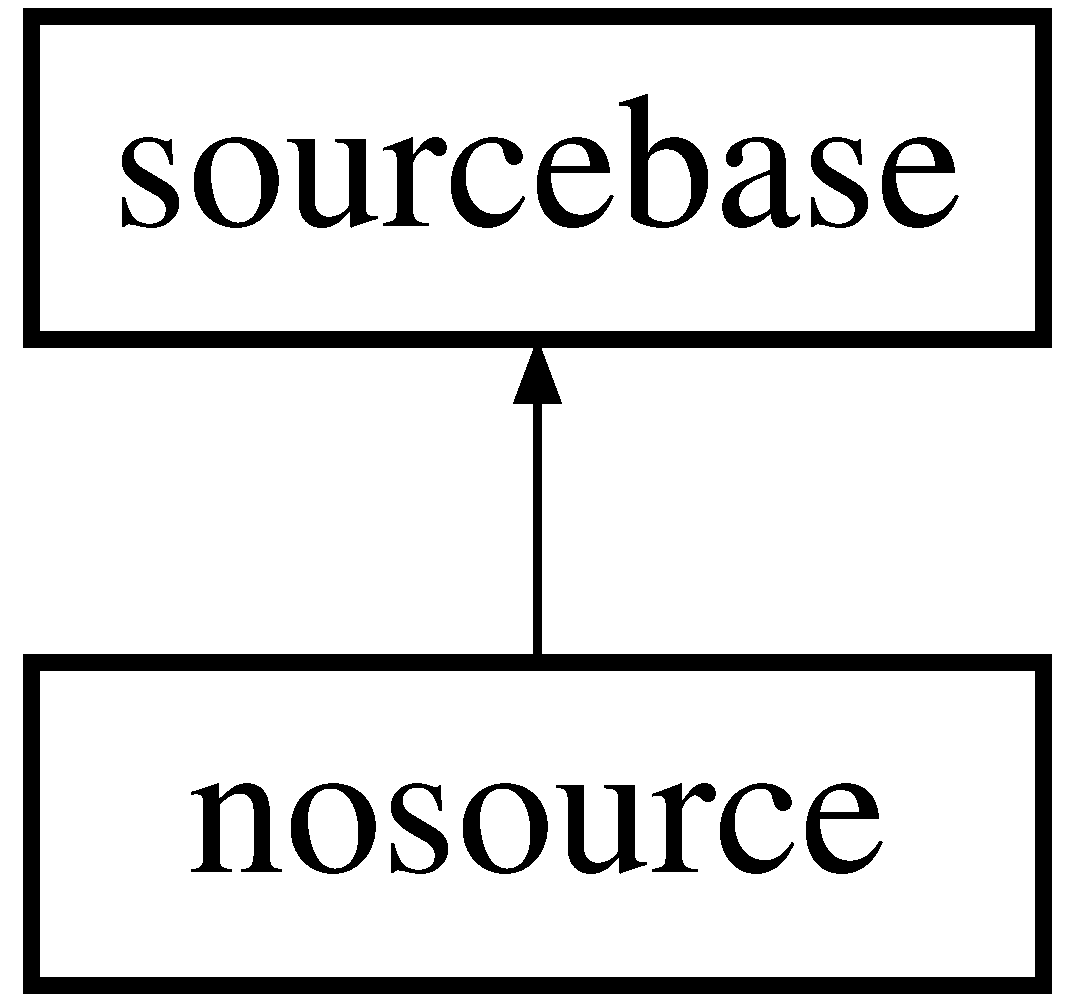
\includegraphics[height=2.000000cm]{classnosource}
\end{center}
\end{figure}
\subsection*{Public Member Functions}
\begin{DoxyCompactItemize}
\item 
void {\bf eval} (double $\ast$, double $\ast$, double $\ast$, double $\ast$)
\begin{DoxyCompactList}\small\item\em Evaluation of the source which does nothing. \end{DoxyCompactList}\end{DoxyCompactItemize}


\subsection{Detailed Description}
Derived No\-Source Class from Source\-Base. 

\subsection{Member Function Documentation}
\index{nosource@{nosource}!eval@{eval}}
\index{eval@{eval}!nosource@{nosource}}
\subsubsection[{eval}]{\setlength{\rightskip}{0pt plus 5cm}void nosource\-::eval (
\begin{DoxyParamCaption}
\item[{double $\ast$}]{, }
\item[{double $\ast$}]{, }
\item[{double $\ast$}]{, }
\item[{double $\ast$}]{}
\end{DoxyParamCaption}
)\hspace{0.3cm}{\ttfamily [inline]}, {\ttfamily [virtual]}}\label{classnosource_ad3c033fef6af9125e0e1959e13a9a0e0}


Evaluation of the source which does nothing. 



Implements {\bf sourcebase} \doxyref{}{p.}{classsourcebase_aa47f29eea4fb554586279a5fa9394cb6}.



The documentation for this class was generated from the following file\-:\begin{DoxyCompactItemize}
\item 
{\bf source.\-h}\end{DoxyCompactItemize}

\section{sedimentdiffusion Class Reference}
\label{classsedimentdiffusion}\index{sedimentdiffusion@{sedimentdiffusion}}


L\-D\-G diffusion flux class used in comination with Grass Bed Updating equation.  




{\ttfamily \#include $<$flux2.\-h$>$}

Inheritance diagram for sedimentdiffusion\-:\begin{figure}[H]
\begin{center}
\leavevmode
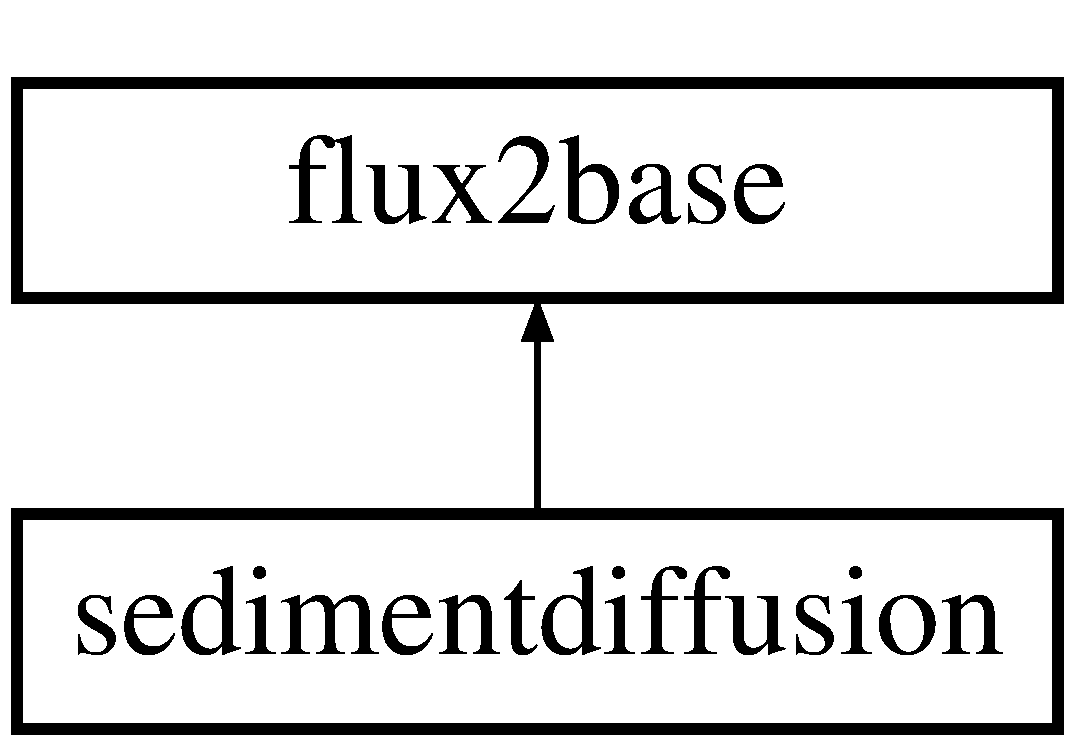
\includegraphics[height=2.000000cm]{classsedimentdiffusion}
\end{center}
\end{figure}
\subsection*{Public Member Functions}
\begin{DoxyCompactItemize}
\item 
double {\bf eval} (double $\ast$, double $\ast$, double $\ast$)
\begin{DoxyCompactList}\small\item\em Evaluates the flux for the L\-D\-G variables for the sedimentdifussion. \end{DoxyCompactList}\end{DoxyCompactItemize}


\subsection{Detailed Description}
L\-D\-G diffusion flux class used in comination with Grass Bed Updating equation. 

\subsection{Member Function Documentation}
\index{sedimentdiffusion@{sedimentdiffusion}!eval@{eval}}
\index{eval@{eval}!sedimentdiffusion@{sedimentdiffusion}}
\subsubsection[{eval}]{\setlength{\rightskip}{0pt plus 5cm}double sedimentdiffusion\-::eval (
\begin{DoxyParamCaption}
\item[{double $\ast$}]{F, }
\item[{double $\ast$}]{u\-L, }
\item[{double $\ast$}]{u\-R}
\end{DoxyParamCaption}
)\hspace{0.3cm}{\ttfamily [virtual]}}\label{classsedimentdiffusion_a99e5ded19d1a705b9eda6d0983de22ff}


Evaluates the flux for the L\-D\-G variables for the sedimentdifussion. 



Implements {\bf flux2base} \doxyref{}{p.}{classflux2base_a4ecfc0d7470722ef299fa054c926f540}.



References element\-::systemsize2.



The documentation for this class was generated from the following files\-:\begin{DoxyCompactItemize}
\item 
{\bf flux2.\-h}\item 
{\bf flux2.\-cpp}\end{DoxyCompactItemize}

\section{sedimenttransport Class Reference}
\label{classsedimenttransport}\index{sedimenttransport@{sedimenttransport}}


Derived fluxbase class for sediment transport.  




{\ttfamily \#include $<$flux.\-h$>$}

Inheritance diagram for sedimenttransport\-:\begin{figure}[H]
\begin{center}
\leavevmode
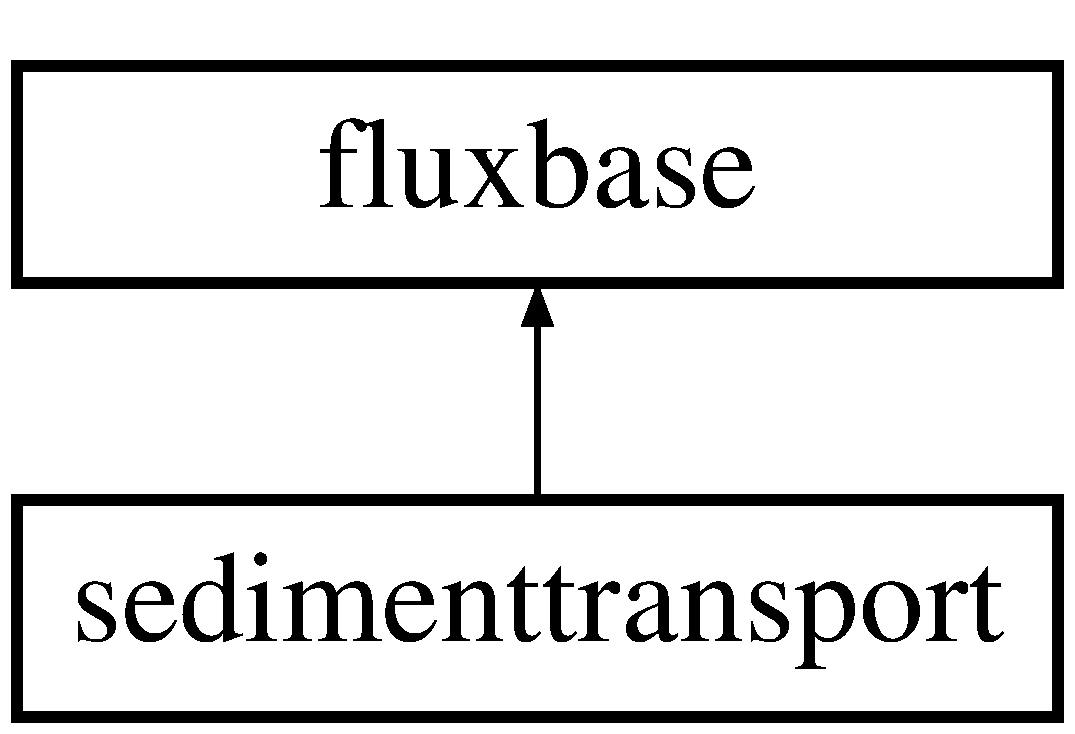
\includegraphics[height=2.000000cm]{classsedimenttransport}
\end{center}
\end{figure}
\subsection*{Public Member Functions}
\begin{DoxyCompactItemize}
\item 
double {\bf eval} (double $\ast$, double $\ast$, double $\ast$, double $\ast$, double $\ast$)
\begin{DoxyCompactList}\small\item\em Evaluation of the ... flux with topography correction. \end{DoxyCompactList}\item 
void {\bf eval\-\_\-l} (double $\ast$, double $\ast$, double $\ast$, double $\ast$, double $\ast$)
\begin{DoxyCompactList}\small\item\em Non conservative flux as suggested by Bouchut et al. (2004). \end{DoxyCompactList}\item 
void {\bf eval\-\_\-r} (double $\ast$, double $\ast$, double $\ast$, double $\ast$, double $\ast$)
\begin{DoxyCompactList}\small\item\em Non conservative flux as suggested by Bouchut et al. (2004). \end{DoxyCompactList}\end{DoxyCompactItemize}


\subsection{Detailed Description}
Derived fluxbase class for sediment transport. 

\subsection{Member Function Documentation}
\index{sedimenttransport@{sedimenttransport}!eval@{eval}}
\index{eval@{eval}!sedimenttransport@{sedimenttransport}}
\subsubsection[{eval}]{\setlength{\rightskip}{0pt plus 5cm}double sedimenttransport\-::eval (
\begin{DoxyParamCaption}
\item[{double $\ast$}]{F, }
\item[{double $\ast$}]{u\-L, }
\item[{double $\ast$}]{u\-R, }
\item[{double $\ast$}]{q\-L, }
\item[{double $\ast$}]{q\-R}
\end{DoxyParamCaption}
)\hspace{0.3cm}{\ttfamily [virtual]}}\label{classsedimenttransport_a05b589c655e8dd393a49acd530bf1e4f}


Evaluation of the ... flux with topography correction. 



Implements {\bf fluxbase} \doxyref{}{p.}{classfluxbase_ab41e8752c750488dbcbc8ef24e277110}.



References Grass\-\_\-const, Grass\-\_\-exponent, gravity\-\_\-const, and element\-::systemsize1.

\index{sedimenttransport@{sedimenttransport}!eval\-\_\-l@{eval\-\_\-l}}
\index{eval\-\_\-l@{eval\-\_\-l}!sedimenttransport@{sedimenttransport}}
\subsubsection[{eval\-\_\-l}]{\setlength{\rightskip}{0pt plus 5cm}void sedimenttransport\-::eval\-\_\-l (
\begin{DoxyParamCaption}
\item[{double $\ast$}]{Fl, }
\item[{double $\ast$}]{u\-L, }
\item[{double $\ast$}]{u\-R, }
\item[{double $\ast$}]{q\-L, }
\item[{double $\ast$}]{q\-R}
\end{DoxyParamCaption}
)\hspace{0.3cm}{\ttfamily [virtual]}}\label{classsedimenttransport_a3624de092117d19e1b355493a4059edb}


Non conservative flux as suggested by Bouchut et al. (2004). 



Implements {\bf fluxbase} \doxyref{}{p.}{classfluxbase_a184e5d5629191871c6dd9cd6b4e82799}.



References gravity\-\_\-const, and element\-::systemsize1.

\index{sedimenttransport@{sedimenttransport}!eval\-\_\-r@{eval\-\_\-r}}
\index{eval\-\_\-r@{eval\-\_\-r}!sedimenttransport@{sedimenttransport}}
\subsubsection[{eval\-\_\-r}]{\setlength{\rightskip}{0pt plus 5cm}void sedimenttransport\-::eval\-\_\-r (
\begin{DoxyParamCaption}
\item[{double $\ast$}]{Fr, }
\item[{double $\ast$}]{u\-L, }
\item[{double $\ast$}]{u\-R, }
\item[{double $\ast$}]{q\-L, }
\item[{double $\ast$}]{q\-R}
\end{DoxyParamCaption}
)\hspace{0.3cm}{\ttfamily [virtual]}}\label{classsedimenttransport_a5d1143b0cfff17016fd5eb2acb9fc1b8}


Non conservative flux as suggested by Bouchut et al. (2004). 



Implements {\bf fluxbase} \doxyref{}{p.}{classfluxbase_ab5e6afaa22aff4a1bbbce0bba561fed3}.



References gravity\-\_\-const, and element\-::systemsize1.



The documentation for this class was generated from the following files\-:\begin{DoxyCompactItemize}
\item 
{\bf flux.\-h}\item 
{\bf flux.\-cpp}\end{DoxyCompactItemize}

\section{sourcebase Class Reference}
\label{classsourcebase}\index{sourcebase@{sourcebase}}


Source base class.  




{\ttfamily \#include $<$source.\-h$>$}

Inheritance diagram for sourcebase\-:\begin{figure}[H]
\begin{center}
\leavevmode
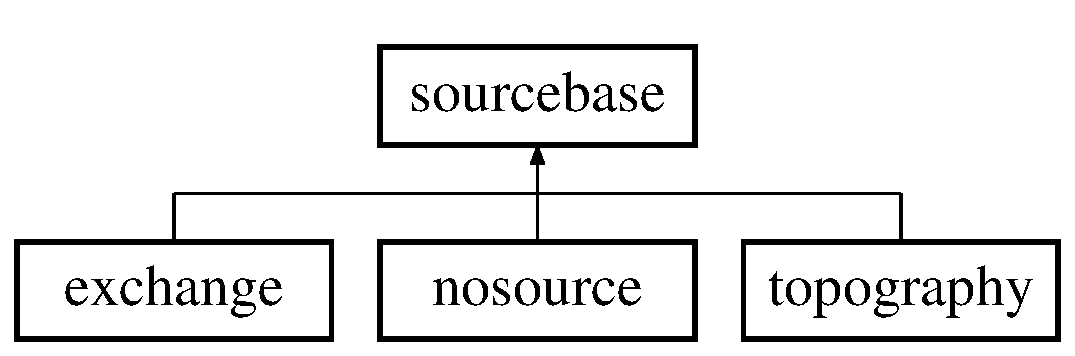
\includegraphics[height=2.000000cm]{classsourcebase}
\end{center}
\end{figure}
\subsection*{Public Member Functions}
\begin{DoxyCompactItemize}
\item 
virtual void {\bf eval} (double $\ast$, double $\ast$, double $\ast$, double $\ast$)=0
\begin{DoxyCompactList}\small\item\em Virtual evaluation of the source. \end{DoxyCompactList}\end{DoxyCompactItemize}


\subsection{Detailed Description}
Source base class. 

\subsection{Member Function Documentation}
\index{sourcebase@{sourcebase}!eval@{eval}}
\index{eval@{eval}!sourcebase@{sourcebase}}
\subsubsection[{eval}]{\setlength{\rightskip}{0pt plus 5cm}virtual void sourcebase\-::eval (
\begin{DoxyParamCaption}
\item[{double $\ast$}]{, }
\item[{double $\ast$}]{, }
\item[{double $\ast$}]{, }
\item[{double $\ast$}]{}
\end{DoxyParamCaption}
)\hspace{0.3cm}{\ttfamily [pure virtual]}}\label{classsourcebase_aa47f29eea4fb554586279a5fa9394cb6}


Virtual evaluation of the source. 



Implemented in {\bf exchange} \doxyref{}{p.}{classexchange_a41c0e65e9f5c985db1672edf390b09e1}, {\bf topography} \doxyref{}{p.}{classtopography_a74a5ec79cd0134dc7c43aa91e81c4669}, and {\bf nosource} \doxyref{}{p.}{classnosource_ad3c033fef6af9125e0e1959e13a9a0e0}.



Referenced by sourceproc().



The documentation for this class was generated from the following file\-:\begin{DoxyCompactItemize}
\item 
{\bf source.\-h}\end{DoxyCompactItemize}

\section{state Class Reference}
\label{classstate}\index{state@{state}}


The state class.  




{\ttfamily \#include $<$state.\-h$>$}

\subsection*{Public Member Functions}
\begin{DoxyCompactItemize}
\item 
{\bf state} ()
\begin{DoxyCompactList}\small\item\em Default constructor\-: creates an empty state vector. \end{DoxyCompactList}\item 
{\bf state} {\bf operator=} ({\bf state} vector)
\begin{DoxyCompactList}\small\item\em Asigns one state vector to another state vector. \end{DoxyCompactList}\item 
double {\bf get} (double)
\begin{DoxyCompactList}\small\item\em Function used to get the value of the state at $\zeta \in [-1,1]$. \end{DoxyCompactList}\item 
double {\bf getslope} (double)
\begin{DoxyCompactList}\small\item\em Function used to get the value of the first derivative of the state at $\zeta \in [-1,1]$. \end{DoxyCompactList}\item 
{\bf state} {\bf clear} ()
\begin{DoxyCompactList}\small\item\em Clears the values in the state vector. \end{DoxyCompactList}\item 
{\bf state} {\bf operator+=} ({\bf state} vector)
\begin{DoxyCompactList}\small\item\em Adds the values of one state vector to another. \end{DoxyCompactList}\item 
{\bf state} {\bf operator$\ast$} (double alpha)
\begin{DoxyCompactList}\small\item\em Multiplies the values in the state vector by $ \alpha $. \end{DoxyCompactList}\item 
{\bf state} {\bf operator/} (double alpha)
\begin{DoxyCompactList}\small\item\em Divides the values in the state vector by $ \alpha $. \end{DoxyCompactList}\end{DoxyCompactItemize}
\subsection*{Public Attributes}
\begin{DoxyCompactItemize}
\item 
double $\ast$ {\bf coefficient}
\begin{DoxyCompactList}\small\item\em Expansion coefficients of state vector. \end{DoxyCompactList}\end{DoxyCompactItemize}
\subsection*{Static Public Attributes}
\begin{DoxyCompactItemize}
\item 
static int {\bf statesize}
\begin{DoxyCompactList}\small\item\em Size of the state vector. \end{DoxyCompactList}\item 
static {\bf state} {\bf g}
\begin{DoxyCompactList}\small\item\em Temporary state vector used to prevent memory overflow. \end{DoxyCompactList}\end{DoxyCompactItemize}


\subsection{Detailed Description}
The state class. 

The state describes how each variable in the element class is stored. 

\subsection{Constructor \& Destructor Documentation}
\index{state@{state}!state@{state}}
\index{state@{state}!state@{state}}
\subsubsection[{state}]{\setlength{\rightskip}{0pt plus 5cm}state\-::state (
\begin{DoxyParamCaption}
{}
\end{DoxyParamCaption}
)}\label{classstate_aee920d9f534640451f22b3525f9cb9de}


Default constructor\-: creates an empty state vector. 



References statesize.



\subsection{Member Function Documentation}
\index{state@{state}!clear@{clear}}
\index{clear@{clear}!state@{state}}
\subsubsection[{clear}]{\setlength{\rightskip}{0pt plus 5cm}{\bf state} state\-::clear (
\begin{DoxyParamCaption}
{}
\end{DoxyParamCaption}
)}\label{classstate_a353c4810f55772b6cdb3df21ee964410}


Clears the values in the state vector. 



References statesize.

\index{state@{state}!get@{get}}
\index{get@{get}!state@{state}}
\subsubsection[{get}]{\setlength{\rightskip}{0pt plus 5cm}double state\-::get (
\begin{DoxyParamCaption}
\item[{double}]{xi}
\end{DoxyParamCaption}
)}\label{classstate_abc460a3926b7e942b805ffc30ecf461e}


Function used to get the value of the state at $\zeta \in [-1,1]$. 



References statesize.

\index{state@{state}!getslope@{getslope}}
\index{getslope@{getslope}!state@{state}}
\subsubsection[{getslope}]{\setlength{\rightskip}{0pt plus 5cm}double state\-::getslope (
\begin{DoxyParamCaption}
\item[{double}]{xi}
\end{DoxyParamCaption}
)}\label{classstate_a13193647ae49dee6ca6fecf12a7015c0}


Function used to get the value of the first derivative of the state at $\zeta \in [-1,1]$. 



References statesize.

\index{state@{state}!operator$\ast$@{operator$\ast$}}
\index{operator$\ast$@{operator$\ast$}!state@{state}}
\subsubsection[{operator$\ast$}]{\setlength{\rightskip}{0pt plus 5cm}{\bf state} state\-::operator$\ast$ (
\begin{DoxyParamCaption}
\item[{double}]{alpha}
\end{DoxyParamCaption}
)}\label{classstate_ad6ad6605800d74976d440523c3e49fbd}


Multiplies the values in the state vector by $ \alpha $. 



References coefficient, and statesize.

\index{state@{state}!operator+=@{operator+=}}
\index{operator+=@{operator+=}!state@{state}}
\subsubsection[{operator+=}]{\setlength{\rightskip}{0pt plus 5cm}{\bf state} state\-::operator+= (
\begin{DoxyParamCaption}
\item[{{\bf state}}]{vector}
\end{DoxyParamCaption}
)}\label{classstate_ab5093775179d037d1ff1d344c6676cd5}


Adds the values of one state vector to another. 



References coefficient, and statesize.

\index{state@{state}!operator/@{operator/}}
\index{operator/@{operator/}!state@{state}}
\subsubsection[{operator/}]{\setlength{\rightskip}{0pt plus 5cm}{\bf state} state\-::operator/ (
\begin{DoxyParamCaption}
\item[{double}]{alpha}
\end{DoxyParamCaption}
)}\label{classstate_a9198637d75028fd110a8fcff2c603a4d}


Divides the values in the state vector by $ \alpha $. 



References coefficient, and statesize.

\index{state@{state}!operator=@{operator=}}
\index{operator=@{operator=}!state@{state}}
\subsubsection[{operator=}]{\setlength{\rightskip}{0pt plus 5cm}{\bf state} state\-::operator= (
\begin{DoxyParamCaption}
\item[{{\bf state}}]{vector}
\end{DoxyParamCaption}
)}\label{classstate_a224738537429b8b9a0bad9cb7d4eff21}


Asigns one state vector to another state vector. 



References coefficient, and statesize.



\subsection{Member Data Documentation}
\index{state@{state}!coefficient@{coefficient}}
\index{coefficient@{coefficient}!state@{state}}
\subsubsection[{coefficient}]{\setlength{\rightskip}{0pt plus 5cm}double$\ast$ state\-::coefficient}\label{classstate_a8f5ab6d0115153b989be84a9a9223359}


Expansion coefficients of state vector. 



Referenced by initcon(), operator$\ast$(), operator+=(), operator/(), and operator=().

\index{state@{state}!g@{g}}
\index{g@{g}!state@{state}}
\subsubsection[{g}]{\setlength{\rightskip}{0pt plus 5cm}{\bf state} state\-::g\hspace{0.3cm}{\ttfamily [static]}}\label{classstate_a9cbd418203ac7d99a1d81fd5281f4c27}


Temporary state vector used to prevent memory overflow. 

\index{state@{state}!statesize@{statesize}}
\index{statesize@{statesize}!state@{state}}
\subsubsection[{statesize}]{\setlength{\rightskip}{0pt plus 5cm}int state\-::statesize\hspace{0.3cm}{\ttfamily [static]}}\label{classstate_a5360a31f6ea76abdb3308ef67c0fd5c7}


Size of the state vector. 



Referenced by clear(), cranknicolsonwp(), eulerforw(), flux2proc(), fluxproc(), get(), getslope(), initcon(), main(), operator$\ast$(), operator+=(), operator/(), operator=(), rk3(), sourceproc(), and state().



The documentation for this class was generated from the following files\-:\begin{DoxyCompactItemize}
\item 
{\bf state.\-h}\item 
{\bf state.\-cpp}\end{DoxyCompactItemize}

\section{suspendedsediment Class Reference}
\label{classsuspendedsediment}\index{suspendedsediment@{suspendedsediment}}


{\ttfamily \#include $<$flux.\-h$>$}

Inheritance diagram for suspendedsediment\-:\begin{figure}[H]
\begin{center}
\leavevmode
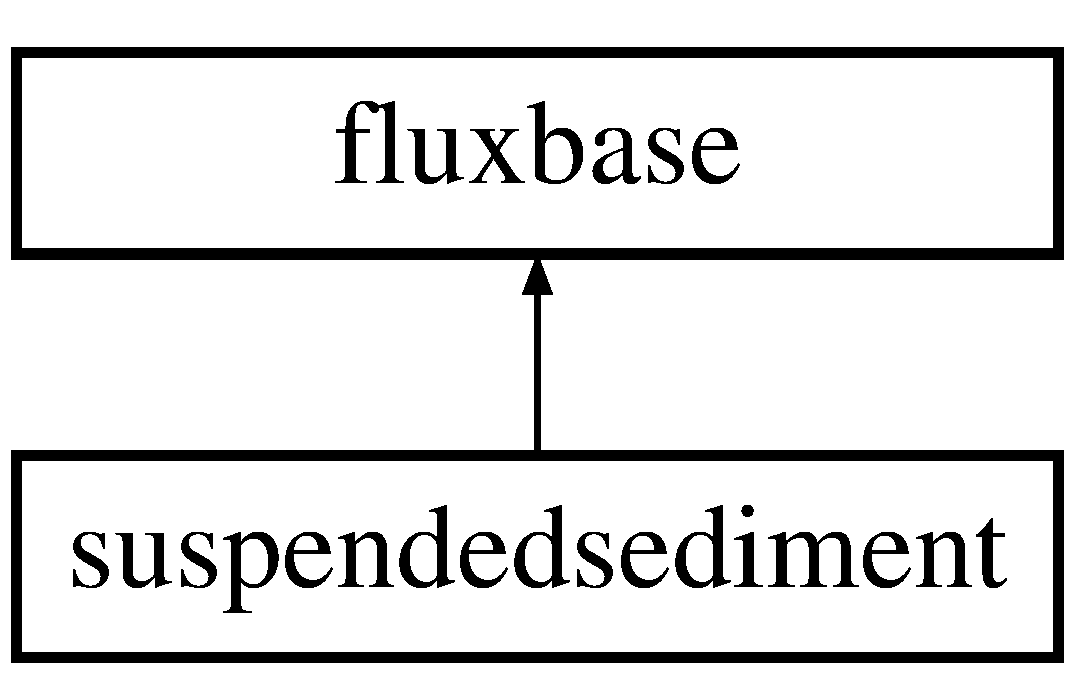
\includegraphics[height=2.000000cm]{classsuspendedsediment}
\end{center}
\end{figure}
\subsection*{Public Member Functions}
\begin{DoxyCompactItemize}
\item 
double {\bf eval} (double $\ast$, double $\ast$, double $\ast$, double $\ast$, double $\ast$)
\begin{DoxyCompactList}\small\item\em Evaluation of the H\-L\-L\-C flux with topography correction. \end{DoxyCompactList}\item 
void {\bf eval\-\_\-l} (double $\ast$, double $\ast$, double $\ast$, double $\ast$, double $\ast$)
\begin{DoxyCompactList}\small\item\em Non conservative flux as suggested by Bouchut et al. (2004). \end{DoxyCompactList}\item 
void {\bf eval\-\_\-r} (double $\ast$, double $\ast$, double $\ast$, double $\ast$, double $\ast$)
\begin{DoxyCompactList}\small\item\em Non conservative flux as suggested by Bouchut et al. (2004). \end{DoxyCompactList}\end{DoxyCompactItemize}


\subsection{Member Function Documentation}
\index{suspendedsediment@{suspendedsediment}!eval@{eval}}
\index{eval@{eval}!suspendedsediment@{suspendedsediment}}
\subsubsection[{eval}]{\setlength{\rightskip}{0pt plus 5cm}double suspendedsediment\-::eval (
\begin{DoxyParamCaption}
\item[{double $\ast$}]{F, }
\item[{double $\ast$}]{u\-L, }
\item[{double $\ast$}]{u\-R, }
\item[{double $\ast$}]{q\-L, }
\item[{double $\ast$}]{q\-R}
\end{DoxyParamCaption}
)\hspace{0.3cm}{\ttfamily [virtual]}}\label{classsuspendedsediment_a26e0411516045d46bc504acc7407797e}


Evaluation of the H\-L\-L\-C flux with topography correction. 



Implements {\bf fluxbase} \doxyref{}{p.}{classfluxbase_ab41e8752c750488dbcbc8ef24e277110}.



References gravity\-\_\-const, and element\-::systemsize1.

\index{suspendedsediment@{suspendedsediment}!eval\-\_\-l@{eval\-\_\-l}}
\index{eval\-\_\-l@{eval\-\_\-l}!suspendedsediment@{suspendedsediment}}
\subsubsection[{eval\-\_\-l}]{\setlength{\rightskip}{0pt plus 5cm}void suspendedsediment\-::eval\-\_\-l (
\begin{DoxyParamCaption}
\item[{double $\ast$}]{Fl, }
\item[{double $\ast$}]{u\-L, }
\item[{double $\ast$}]{u\-R, }
\item[{double $\ast$}]{q\-L, }
\item[{double $\ast$}]{q\-R}
\end{DoxyParamCaption}
)\hspace{0.3cm}{\ttfamily [virtual]}}\label{classsuspendedsediment_af4d3a3daf5a292a36b438512704d4098}


Non conservative flux as suggested by Bouchut et al. (2004). 



Implements {\bf fluxbase} \doxyref{}{p.}{classfluxbase_a184e5d5629191871c6dd9cd6b4e82799}.



References gravity\-\_\-const, and element\-::systemsize1.

\index{suspendedsediment@{suspendedsediment}!eval\-\_\-r@{eval\-\_\-r}}
\index{eval\-\_\-r@{eval\-\_\-r}!suspendedsediment@{suspendedsediment}}
\subsubsection[{eval\-\_\-r}]{\setlength{\rightskip}{0pt plus 5cm}void suspendedsediment\-::eval\-\_\-r (
\begin{DoxyParamCaption}
\item[{double $\ast$}]{Fr, }
\item[{double $\ast$}]{u\-L, }
\item[{double $\ast$}]{u\-R, }
\item[{double $\ast$}]{q\-L, }
\item[{double $\ast$}]{q\-R}
\end{DoxyParamCaption}
)\hspace{0.3cm}{\ttfamily [virtual]}}\label{classsuspendedsediment_a232c9be4aad28973ade9e46222489035}


Non conservative flux as suggested by Bouchut et al. (2004). 



Implements {\bf fluxbase} \doxyref{}{p.}{classfluxbase_ab5e6afaa22aff4a1bbbce0bba561fed3}.



References gravity\-\_\-const, and element\-::systemsize1.



The documentation for this class was generated from the following files\-:\begin{DoxyCompactItemize}
\item 
{\bf flux.\-h}\item 
{\bf flux.\-cpp}\end{DoxyCompactItemize}

\section{swehllc Class Reference}
\label{classswehllc}\index{swehllc@{swehllc}}


Derived fluxbase class for Shallow Water equations using H\-L\-L\-C with no topography.  




{\ttfamily \#include $<$flux.\-h$>$}

Inheritance diagram for swehllc\-:\begin{figure}[H]
\begin{center}
\leavevmode
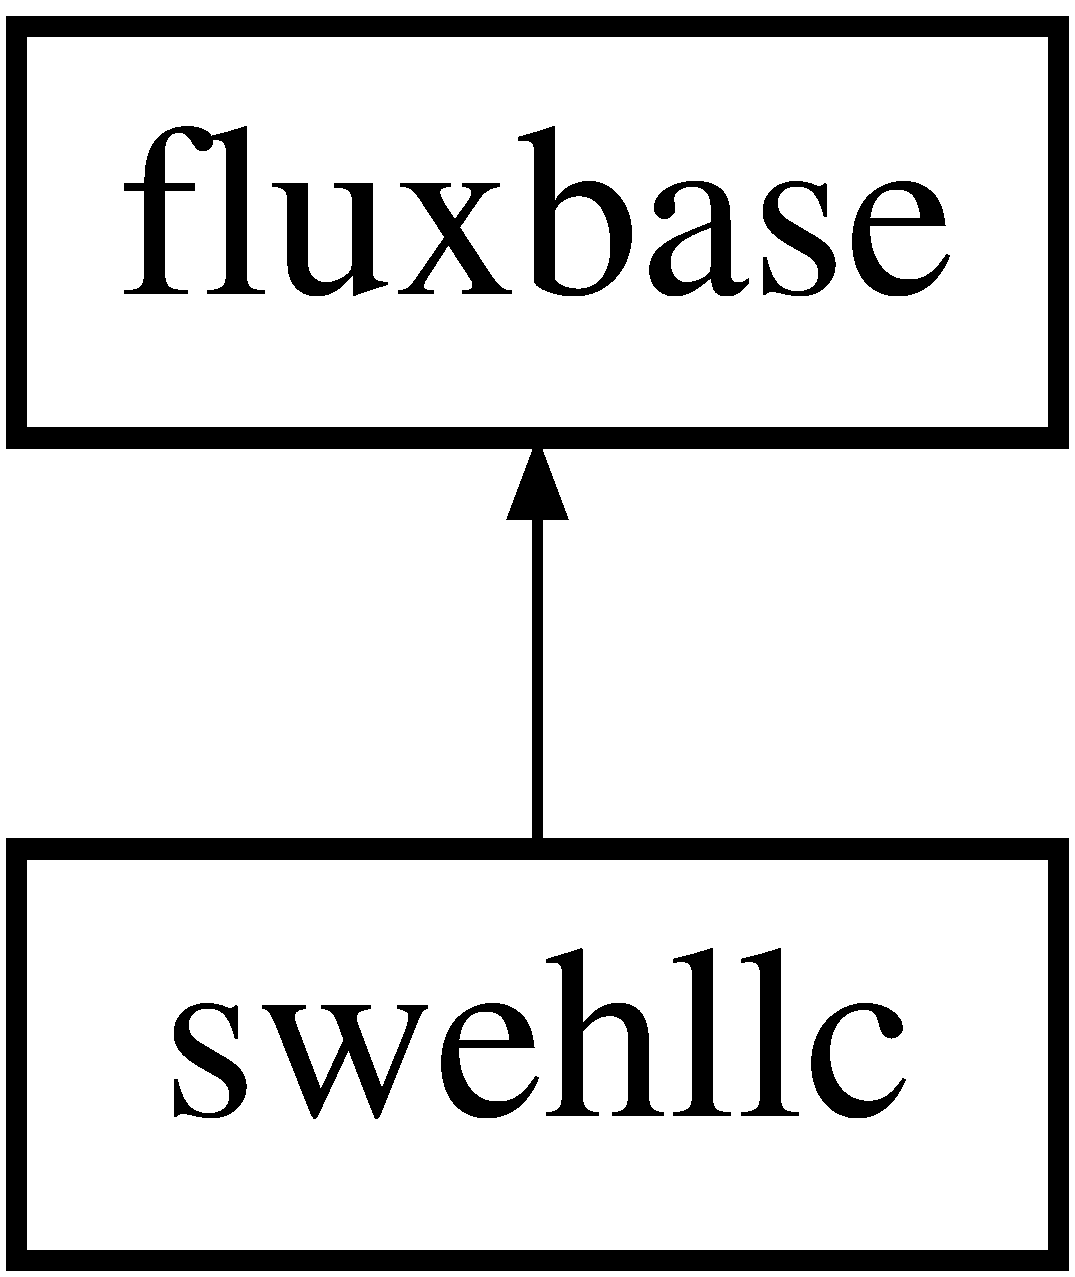
\includegraphics[height=2.000000cm]{classswehllc}
\end{center}
\end{figure}
\subsection*{Public Member Functions}
\begin{DoxyCompactItemize}
\item 
double {\bf eval} (double $\ast$, double $\ast$, double $\ast$, double $\ast$, double $\ast$)
\begin{DoxyCompactList}\small\item\em Evaluation of the H\-L\-L\-C flux. \end{DoxyCompactList}\item 
void {\bf eval\-\_\-l} (double $\ast$, double $\ast$, double $\ast$, double $\ast$, double $\ast$)
\begin{DoxyCompactList}\small\item\em Virtual non conservative evaluation of the flux on the left of the element. \end{DoxyCompactList}\item 
void {\bf eval\-\_\-r} (double $\ast$, double $\ast$, double $\ast$, double $\ast$, double $\ast$)
\begin{DoxyCompactList}\small\item\em Virtual non conservative evaluation of the flux on the right of the element. \end{DoxyCompactList}\end{DoxyCompactItemize}


\subsection{Detailed Description}
Derived fluxbase class for Shallow Water equations using H\-L\-L\-C with no topography. 

\subsection{Member Function Documentation}
\index{swehllc@{swehllc}!eval@{eval}}
\index{eval@{eval}!swehllc@{swehllc}}
\subsubsection[{eval}]{\setlength{\rightskip}{0pt plus 5cm}double swehllc\-::eval (
\begin{DoxyParamCaption}
\item[{double $\ast$}]{F, }
\item[{double $\ast$}]{u\-L, }
\item[{double $\ast$}]{u\-R, }
\item[{double $\ast$}]{q\-L, }
\item[{double $\ast$}]{q\-R}
\end{DoxyParamCaption}
)\hspace{0.3cm}{\ttfamily [virtual]}}\label{classswehllc_a3cdffa7499fb936220d0084343401cad}


Evaluation of the H\-L\-L\-C flux. 



Implements {\bf fluxbase} \doxyref{}{p.}{classfluxbase_ab41e8752c750488dbcbc8ef24e277110}.



References gravity\-\_\-const, and element\-::systemsize1.

\index{swehllc@{swehllc}!eval\-\_\-l@{eval\-\_\-l}}
\index{eval\-\_\-l@{eval\-\_\-l}!swehllc@{swehllc}}
\subsubsection[{eval\-\_\-l}]{\setlength{\rightskip}{0pt plus 5cm}void swehllc\-::eval\-\_\-l (
\begin{DoxyParamCaption}
\item[{double $\ast$}]{, }
\item[{double $\ast$}]{, }
\item[{double $\ast$}]{, }
\item[{double $\ast$}]{, }
\item[{double $\ast$}]{}
\end{DoxyParamCaption}
)\hspace{0.3cm}{\ttfamily [inline]}, {\ttfamily [virtual]}}\label{classswehllc_abaf31947a1472a531131f2569919a300}


Virtual non conservative evaluation of the flux on the left of the element. 



Implements {\bf fluxbase} \doxyref{}{p.}{classfluxbase_a184e5d5629191871c6dd9cd6b4e82799}.

\index{swehllc@{swehllc}!eval\-\_\-r@{eval\-\_\-r}}
\index{eval\-\_\-r@{eval\-\_\-r}!swehllc@{swehllc}}
\subsubsection[{eval\-\_\-r}]{\setlength{\rightskip}{0pt plus 5cm}void swehllc\-::eval\-\_\-r (
\begin{DoxyParamCaption}
\item[{double $\ast$}]{, }
\item[{double $\ast$}]{, }
\item[{double $\ast$}]{, }
\item[{double $\ast$}]{, }
\item[{double $\ast$}]{}
\end{DoxyParamCaption}
)\hspace{0.3cm}{\ttfamily [inline]}, {\ttfamily [virtual]}}\label{classswehllc_af72fc457d5445284b1cef0cdd28071af}


Virtual non conservative evaluation of the flux on the right of the element. 



Implements {\bf fluxbase} \doxyref{}{p.}{classfluxbase_ab5e6afaa22aff4a1bbbce0bba561fed3}.



The documentation for this class was generated from the following files\-:\begin{DoxyCompactItemize}
\item 
{\bf flux.\-h}\item 
{\bf flux.\-cpp}\end{DoxyCompactItemize}

\section{swehllctopography Class Reference}
\label{classswehllctopography}\index{swehllctopography@{swehllctopography}}


Derived fluxbase class for Shallow Water equations using H\-L\-L\-C with discontinuous topography.  




{\ttfamily \#include $<$flux.\-h$>$}

Inheritance diagram for swehllctopography\-:\begin{figure}[H]
\begin{center}
\leavevmode
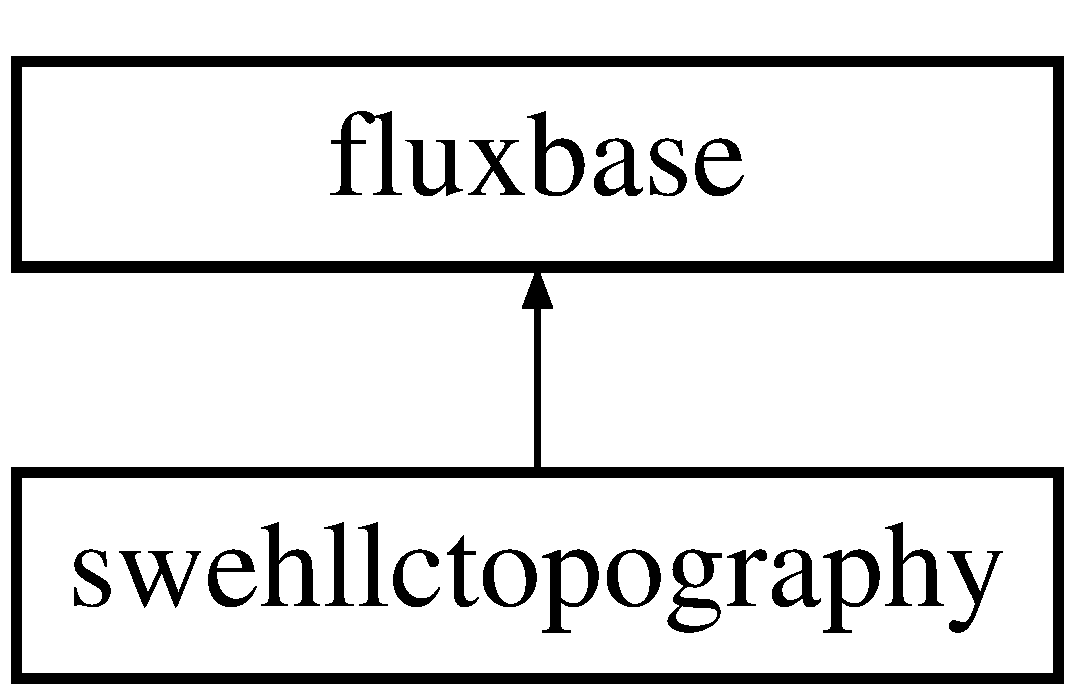
\includegraphics[height=2.000000cm]{classswehllctopography}
\end{center}
\end{figure}
\subsection*{Public Member Functions}
\begin{DoxyCompactItemize}
\item 
double {\bf eval} (double $\ast$, double $\ast$, double $\ast$, double $\ast$, double $\ast$)
\begin{DoxyCompactList}\small\item\em Evaluation of the H\-L\-L\-C flux with topography correction. \end{DoxyCompactList}\item 
void {\bf eval\-\_\-l} (double $\ast$, double $\ast$, double $\ast$, double $\ast$, double $\ast$)
\begin{DoxyCompactList}\small\item\em Non conservative flux as suggested by Bouchut et al. (2004). \end{DoxyCompactList}\item 
void {\bf eval\-\_\-r} (double $\ast$, double $\ast$, double $\ast$, double $\ast$, double $\ast$)
\begin{DoxyCompactList}\small\item\em Non conservative flux as suggested by Bouchut et al. (2004). \end{DoxyCompactList}\end{DoxyCompactItemize}


\subsection{Detailed Description}
Derived fluxbase class for Shallow Water equations using H\-L\-L\-C with discontinuous topography. 

\subsection{Member Function Documentation}
\index{swehllctopography@{swehllctopography}!eval@{eval}}
\index{eval@{eval}!swehllctopography@{swehllctopography}}
\subsubsection[{eval}]{\setlength{\rightskip}{0pt plus 5cm}double swehllctopography\-::eval (
\begin{DoxyParamCaption}
\item[{double $\ast$}]{F, }
\item[{double $\ast$}]{u\-L, }
\item[{double $\ast$}]{u\-R, }
\item[{double $\ast$}]{q\-L, }
\item[{double $\ast$}]{q\-R}
\end{DoxyParamCaption}
)\hspace{0.3cm}{\ttfamily [virtual]}}\label{classswehllctopography_a94451a4ed6ec36f3c79ef8145cc81d47}


Evaluation of the H\-L\-L\-C flux with topography correction. 



Implements {\bf fluxbase} \doxyref{}{p.}{classfluxbase_ab41e8752c750488dbcbc8ef24e277110}.



References gravity\-\_\-const, and element\-::systemsize1.

\index{swehllctopography@{swehllctopography}!eval\-\_\-l@{eval\-\_\-l}}
\index{eval\-\_\-l@{eval\-\_\-l}!swehllctopography@{swehllctopography}}
\subsubsection[{eval\-\_\-l}]{\setlength{\rightskip}{0pt plus 5cm}void swehllctopography\-::eval\-\_\-l (
\begin{DoxyParamCaption}
\item[{double $\ast$}]{Fl, }
\item[{double $\ast$}]{u\-L, }
\item[{double $\ast$}]{u\-R, }
\item[{double $\ast$}]{q\-L, }
\item[{double $\ast$}]{q\-R}
\end{DoxyParamCaption}
)\hspace{0.3cm}{\ttfamily [virtual]}}\label{classswehllctopography_a29fe7da27580e800cebbfb98f2646fc3}


Non conservative flux as suggested by Bouchut et al. (2004). 



Implements {\bf fluxbase} \doxyref{}{p.}{classfluxbase_a184e5d5629191871c6dd9cd6b4e82799}.



References gravity\-\_\-const, and element\-::systemsize1.

\index{swehllctopography@{swehllctopography}!eval\-\_\-r@{eval\-\_\-r}}
\index{eval\-\_\-r@{eval\-\_\-r}!swehllctopography@{swehllctopography}}
\subsubsection[{eval\-\_\-r}]{\setlength{\rightskip}{0pt plus 5cm}void swehllctopography\-::eval\-\_\-r (
\begin{DoxyParamCaption}
\item[{double $\ast$}]{Fr, }
\item[{double $\ast$}]{u\-L, }
\item[{double $\ast$}]{u\-R, }
\item[{double $\ast$}]{q\-L, }
\item[{double $\ast$}]{q\-R}
\end{DoxyParamCaption}
)\hspace{0.3cm}{\ttfamily [virtual]}}\label{classswehllctopography_a858997ee906ad37ec1490abaff502841}


Non conservative flux as suggested by Bouchut et al. (2004). 



Implements {\bf fluxbase} \doxyref{}{p.}{classfluxbase_ab5e6afaa22aff4a1bbbce0bba561fed3}.



References gravity\-\_\-const, and element\-::systemsize1.



The documentation for this class was generated from the following files\-:\begin{DoxyCompactItemize}
\item 
{\bf flux.\-h}\item 
{\bf flux.\-cpp}\end{DoxyCompactItemize}

\section{topography Class Reference}
\label{classtopography}\index{topography@{topography}}


Derived Topography Class from Source\-Base.  




{\ttfamily \#include $<$source.\-h$>$}

Inheritance diagram for topography\-:\begin{figure}[H]
\begin{center}
\leavevmode
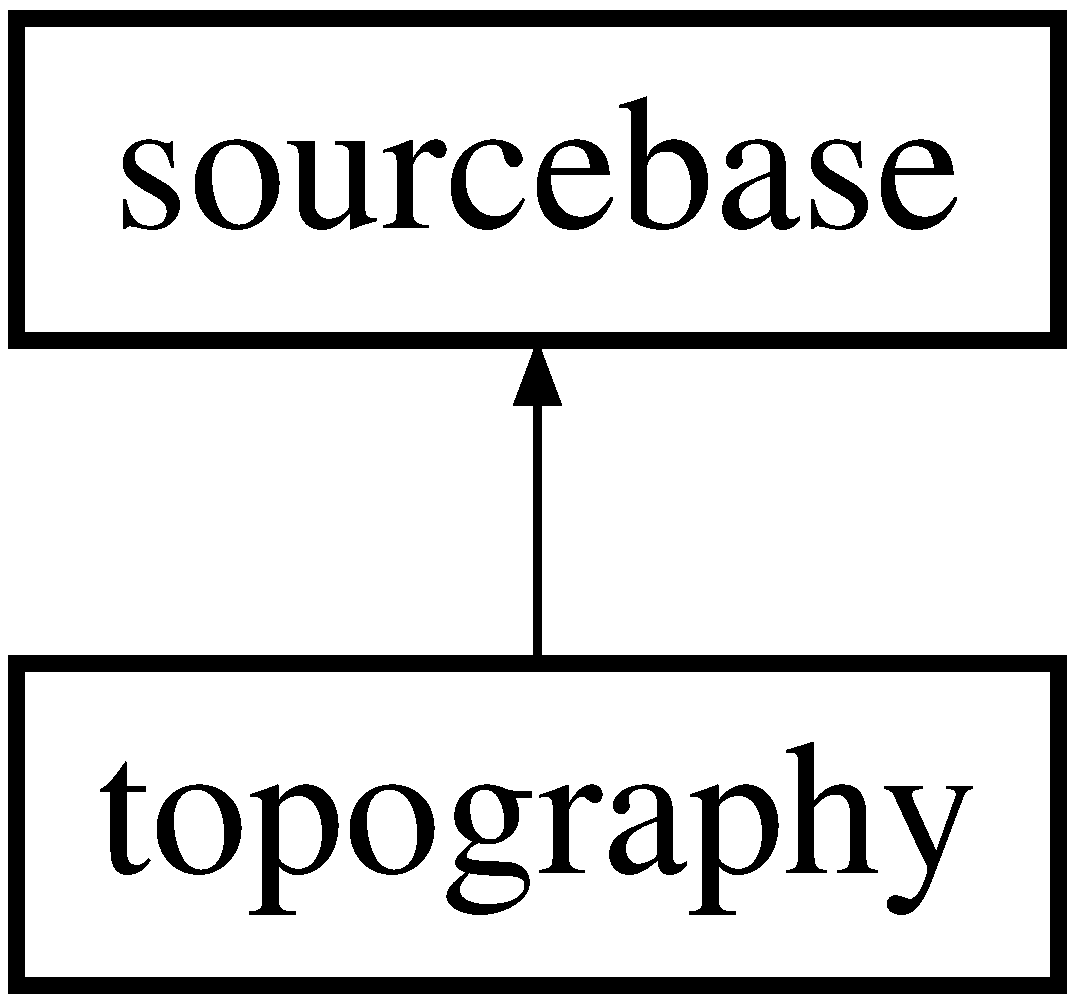
\includegraphics[height=2.000000cm]{classtopography}
\end{center}
\end{figure}
\subsection*{Public Member Functions}
\begin{DoxyCompactItemize}
\item 
void {\bf eval} (double $\ast$, double $\ast$, double $\ast$, double $\ast$)
\begin{DoxyCompactList}\small\item\em Evaluation of the Source in the Shallow Water Equations. \end{DoxyCompactList}\end{DoxyCompactItemize}


\subsection{Detailed Description}
Derived Topography Class from Source\-Base. 

\subsection{Member Function Documentation}
\index{topography@{topography}!eval@{eval}}
\index{eval@{eval}!topography@{topography}}
\subsubsection[{eval}]{\setlength{\rightskip}{0pt plus 5cm}void topography\-::eval (
\begin{DoxyParamCaption}
\item[{double $\ast$}]{F2, }
\item[{double $\ast$}]{u\-L, }
\item[{double $\ast$}]{u\-Lslope, }
\item[{double $\ast$}]{q\-L}
\end{DoxyParamCaption}
)\hspace{0.3cm}{\ttfamily [virtual]}}\label{classtopography_a74a5ec79cd0134dc7c43aa91e81c4669}


Evaluation of the Source in the Shallow Water Equations. 


\begin{DoxyItemize}
\item H\-\_\-0 / (U\-\_\-0)$^\wedge$2; 
\end{DoxyItemize}

Implements {\bf sourcebase} \doxyref{}{p.}{classsourcebase_aa47f29eea4fb554586279a5fa9394cb6}.



References gravity\-\_\-const, and element\-::systemsize1.



The documentation for this class was generated from the following files\-:\begin{DoxyCompactItemize}
\item 
{\bf source.\-h}\item 
{\bf source.\-cpp}\end{DoxyCompactItemize}

\chapter{File Documentation}
\section{cranknicolsonwp.\-cpp File Reference}
\label{cranknicolsonwp_8cpp}\index{cranknicolsonwp.\-cpp@{cranknicolsonwp.\-cpp}}
{\ttfamily \#include $<$vector$>$}\\*
{\ttfamily \#include $<$iostream$>$}\\*
{\ttfamily \#include \char`\"{}node.\-h\char`\"{}}\\*
{\ttfamily \#include \char`\"{}state.\-h\char`\"{}}\\*
{\ttfamily \#include \char`\"{}element.\-h\char`\"{}}\\*
{\ttfamily \#include \char`\"{}source.\-h\char`\"{}}\\*
{\ttfamily \#include \char`\"{}flux.\-h\char`\"{}}\\*
{\ttfamily \#include \char`\"{}flux2.\-h\char`\"{}}\\*
{\ttfamily \#include \char`\"{}fluxproc.\-h\char`\"{}}\\*
{\ttfamily \#include \char`\"{}flux2proc.\-h\char`\"{}}\\*
{\ttfamily \#include \char`\"{}sourceproc.\-h\char`\"{}}\\*
{\ttfamily \#include \char`\"{}cranknicolsonwp.\-h\char`\"{}}\\*
{\ttfamily \#include \char`\"{}updatenodes.\-h\char`\"{}}\\*
\subsection*{Functions}
\begin{DoxyCompactItemize}
\item 
int {\bf cranknicolsonwp} (double \&dt, vector$<$ {\bf node} $>$ \&Nodes, vector$<$ {\bf element} $>$ \&Elements, int bcl, int bcr, {\bf testtypedescr} testtype, {\bf fluxbase} $\ast$fluxtype, {\bf sourcebase} $\ast$sourcetype, {\bf flux2base} $\ast$flux2type, double t)
\end{DoxyCompactItemize}


\subsection{Function Documentation}
\index{cranknicolsonwp.\-cpp@{cranknicolsonwp.\-cpp}!cranknicolsonwp@{cranknicolsonwp}}
\index{cranknicolsonwp@{cranknicolsonwp}!cranknicolsonwp.cpp@{cranknicolsonwp.\-cpp}}
\subsubsection[{cranknicolsonwp}]{\setlength{\rightskip}{0pt plus 5cm}int cranknicolsonwp (
\begin{DoxyParamCaption}
\item[{double \&}]{dt, }
\item[{vector$<$ {\bf node} $>$ \&}]{Nodes, }
\item[{vector$<$ {\bf element} $>$ \&}]{Elements, }
\item[{int}]{bcl, }
\item[{int}]{bcr, }
\item[{{\bf testtypedescr}}]{testtype, }
\item[{{\bf fluxbase} $\ast$}]{fluxtype, }
\item[{{\bf sourcebase} $\ast$}]{sourcetype, }
\item[{{\bf flux2base} $\ast$}]{flux2type, }
\item[{double}]{t}
\end{DoxyParamCaption}
)}\label{cranknicolsonwp_8cpp_a6a037a9a262c7b43bf9cbbd704cfec92}


References flux2proc(), fluxproc(), sourceproc(), state\-::statesize, element\-::systemsize1, and element\-::systemsize2.



Referenced by main().


\section{cranknicolsonwp.\-h File Reference}
\label{cranknicolsonwp_8h}\index{cranknicolsonwp.\-h@{cranknicolsonwp.\-h}}
{\ttfamily \#include \char`\"{}node.\-h\char`\"{}}\\*
{\ttfamily \#include \char`\"{}state.\-h\char`\"{}}\\*
{\ttfamily \#include \char`\"{}element.\-h\char`\"{}}\\*
{\ttfamily \#include \char`\"{}flux.\-h\char`\"{}}\\*
{\ttfamily \#include \char`\"{}source.\-h\char`\"{}}\\*
{\ttfamily \#include \char`\"{}flux2.\-h\char`\"{}}\\*
{\ttfamily \#include $<$vector$>$}\\*
\subsection*{Functions}
\begin{DoxyCompactItemize}
\item 
int {\bf cranknicolsonwp} (double \&dt, vector$<$ {\bf node} $>$ \&Nodes, vector$<$ {\bf element} $>$ \&Element, int bcl, int bcr, {\bf testtypedescr} testtype, {\bf fluxbase} $\ast$fluxtype, {\bf sourcebase} $\ast$sourcetype, {\bf flux2base} $\ast$flux2type, double t)
\end{DoxyCompactItemize}


\subsection{Function Documentation}
\index{cranknicolsonwp.\-h@{cranknicolsonwp.\-h}!cranknicolsonwp@{cranknicolsonwp}}
\index{cranknicolsonwp@{cranknicolsonwp}!cranknicolsonwp.h@{cranknicolsonwp.\-h}}
\subsubsection[{cranknicolsonwp}]{\setlength{\rightskip}{0pt plus 5cm}int cranknicolsonwp (
\begin{DoxyParamCaption}
\item[{double \&}]{dt, }
\item[{vector$<$ {\bf node} $>$ \&}]{Nodes, }
\item[{vector$<$ {\bf element} $>$ \&}]{Element, }
\item[{int}]{bcl, }
\item[{int}]{bcr, }
\item[{{\bf testtypedescr}}]{testtype, }
\item[{{\bf fluxbase} $\ast$}]{fluxtype, }
\item[{{\bf sourcebase} $\ast$}]{sourcetype, }
\item[{{\bf flux2base} $\ast$}]{flux2type, }
\item[{double}]{t}
\end{DoxyParamCaption}
)}\label{cranknicolsonwp_8h_afdc3993f129d26308e4cbfe4b56f0858}


References flux2proc(), fluxproc(), sourceproc(), state\-::statesize, element\-::systemsize1, and element\-::systemsize2.



Referenced by main().


\section{element.\-cpp File Reference}
\label{element_8cpp}\index{element.\-cpp@{element.\-cpp}}
{\ttfamily \#include $<$iostream$>$}\\*
{\ttfamily \#include $<$math.\-h$>$}\\*
{\ttfamily \#include \char`\"{}state.\-h\char`\"{}}\\*
{\ttfamily \#include \char`\"{}element.\-h\char`\"{}}\\*

\section{element.\-h File Reference}
\label{element_8h}\index{element.\-h@{element.\-h}}
{\ttfamily \#include \char`\"{}state.\-h\char`\"{}}\\*
\subsection*{Classes}
\begin{DoxyCompactItemize}
\item 
class {\bf element}
\begin{DoxyCompactList}\small\item\em The element class. \end{DoxyCompactList}\end{DoxyCompactItemize}

\section{enumtypes.\-cpp File Reference}
\label{enumtypes_8cpp}\index{enumtypes.\-cpp@{enumtypes.\-cpp}}
\subsection*{Enumerations}
\begin{DoxyCompactItemize}
\item 
enum {\bf timeintmethod} \{ \\*
{\bf Euler\-Forward}, 
{\bf Runge\-Kutta3}, 
{\bf Crank\-Nicolson\-With\-Predictor}, 
{\bf Euler\-Forward}, 
\\*
{\bf Runge\-Kutta3}, 
{\bf Crank\-Nicolson\-With\-Predictor}
 \}
\item 
enum {\bf testtypedescr} \{ \\*
{\bf Advection}, 
{\bf Burgers}, 
{\bf S\-W\-E\-Burgers}, 
{\bf S\-W\-E\-Linear\-Wave\-Solution}, 
\\*
{\bf S\-W\-E\-Riemann\-Problem\-Left\-Rarefaction\-Right\-Shock}, 
{\bf S\-W\-E\-Riemann\-Problem\-Left\-Shock\-Right\-Rarefaction}, 
{\bf S\-W\-E\-Riemann\-Problem\-Left\-Shock\-Right\-Shock}, 
{\bf S\-W\-E\-Riemann\-Problem\-Left\-Rarefaction\-Right\-Rarefaction}, 
\\*
{\bf S\-W\-E\-Continuous\-Topography}, 
{\bf S\-W\-E\-Discontinuous\-Topography}, 
{\bf S\-W\-E\-Flow\-Over\-Isolated\-Continuous\-Ridge\-I}, 
{\bf S\-W\-E\-Flow\-Over\-Isolated\-Discontinuous\-Ridge\-I}, 
\\*
{\bf S\-W\-E\-Flow\-Over\-Isolated\-Continuous\-Ridge\-I\-V}, 
{\bf S\-W\-E\-Flow\-Over\-Isolated\-Discontinuous\-Ridge\-I\-V}, 
{\bf Burgers\-Diffusive}, 
{\bf Sediment\-Transport}, 
\\*
{\bf H\-L\-L\-Grass}, 
{\bf L\-F\-Grass}, 
{\bf L\-F\-Grass\-Momentum}, 
{\bf Decoupled\-Grass\-Sediment\-Only}, 
\\*
{\bf Suspended\-Sediment}, 
{\bf L\-F\-Grass\-Momentum\-Diffusion}, 
{\bf S\-W\-E\-Flow\-Over\-Siny\-Bed\-I}, 
{\bf Advection}, 
\\*
{\bf Burgers}, 
{\bf S\-W\-E\-Burgers}, 
{\bf S\-W\-E\-Linear\-Wave\-Solution}, 
{\bf S\-W\-E\-Riemann\-Problem\-Left\-Rarefaction\-Right\-Shock}, 
\\*
{\bf S\-W\-E\-Riemann\-Problem\-Left\-Shock\-Right\-Rarefaction}, 
{\bf S\-W\-E\-Riemann\-Problem\-Left\-Shock\-Right\-Shock}, 
{\bf S\-W\-E\-Riemann\-Problem\-Left\-Rarefaction\-Right\-Rarefaction}, 
{\bf S\-W\-E\-Continuous\-Topography}, 
\\*
{\bf S\-W\-E\-Discontinuous\-Topography}, 
{\bf S\-W\-E\-Flow\-Over\-Isolated\-Continuous\-Ridge\-I}, 
{\bf S\-W\-E\-Flow\-Over\-Isolated\-Discontinuous\-Ridge\-I}, 
{\bf S\-W\-E\-Flow\-Over\-Isolated\-Continuous\-Ridge\-I\-V}, 
\\*
{\bf S\-W\-E\-Flow\-Over\-Isolated\-Discontinuous\-Ridge\-I\-V}, 
{\bf Burgers\-Diffusive}, 
{\bf Sediment\-Transport}, 
{\bf H\-L\-L\-Grass}, 
\\*
{\bf L\-F\-Grass}, 
{\bf L\-F\-Grass\-Momentum}, 
{\bf Decoupled\-Grass\-Sediment\-Only}, 
{\bf Suspended\-Sediment}, 
\\*
{\bf L\-F\-Grass\-Momentum\-Diffusion}, 
{\bf S\-W\-E\-Flow\-Over\-Siny\-Bed\-I}
 \}
\item 
enum {\bf boundarycondition} \{ \\*
{\bf Periodic}, 
{\bf Transmissive}, 
{\bf Wall}, 
{\bf Prescribed}, 
\\*
{\bf Periodic}, 
{\bf Transmissive}, 
{\bf Wall}, 
{\bf Prescribed}
 \}
\end{DoxyCompactItemize}


\subsection{Enumeration Type Documentation}
\index{enumtypes.\-cpp@{enumtypes.\-cpp}!boundarycondition@{boundarycondition}}
\index{boundarycondition@{boundarycondition}!enumtypes.cpp@{enumtypes.\-cpp}}
\subsubsection[{boundarycondition}]{\setlength{\rightskip}{0pt plus 5cm}enum {\bf boundarycondition}}\label{enumtypes_8cpp_a8417eaee8c90ff931dfc45f62364e84b}
\begin{Desc}
\item[Enumerator]\par
\begin{description}
\index{Periodic@{Periodic}!enumtypes.\-cpp@{enumtypes.\-cpp}}\index{enumtypes.\-cpp@{enumtypes.\-cpp}!Periodic@{Periodic}}\item[{\em 
Periodic\label{enumtypes_8cpp_a8417eaee8c90ff931dfc45f62364e84ba6db09e3bc054df6f996a45de2ccfeacd}
}]\index{Transmissive@{Transmissive}!enumtypes.\-cpp@{enumtypes.\-cpp}}\index{enumtypes.\-cpp@{enumtypes.\-cpp}!Transmissive@{Transmissive}}\item[{\em 
Transmissive\label{enumtypes_8cpp_a8417eaee8c90ff931dfc45f62364e84ba2d406f2116c0d306d3ca8d9cb2a4a026}
}]\index{Wall@{Wall}!enumtypes.\-cpp@{enumtypes.\-cpp}}\index{enumtypes.\-cpp@{enumtypes.\-cpp}!Wall@{Wall}}\item[{\em 
Wall\label{enumtypes_8cpp_a8417eaee8c90ff931dfc45f62364e84ba5587855d9c996218f85bf20a8bd424d0}
}]\index{Prescribed@{Prescribed}!enumtypes.\-cpp@{enumtypes.\-cpp}}\index{enumtypes.\-cpp@{enumtypes.\-cpp}!Prescribed@{Prescribed}}\item[{\em 
Prescribed\label{enumtypes_8cpp_a8417eaee8c90ff931dfc45f62364e84ba8a8bb2426ed030675d824b7eb4ac2dd7}
}]\index{Periodic@{Periodic}!enumtypes.\-cpp@{enumtypes.\-cpp}}\index{enumtypes.\-cpp@{enumtypes.\-cpp}!Periodic@{Periodic}}\item[{\em 
Periodic\label{enumtypes_8cpp_a8417eaee8c90ff931dfc45f62364e84ba6db09e3bc054df6f996a45de2ccfeacd}
}]\index{Transmissive@{Transmissive}!enumtypes.\-cpp@{enumtypes.\-cpp}}\index{enumtypes.\-cpp@{enumtypes.\-cpp}!Transmissive@{Transmissive}}\item[{\em 
Transmissive\label{enumtypes_8cpp_a8417eaee8c90ff931dfc45f62364e84ba2d406f2116c0d306d3ca8d9cb2a4a026}
}]\index{Wall@{Wall}!enumtypes.\-cpp@{enumtypes.\-cpp}}\index{enumtypes.\-cpp@{enumtypes.\-cpp}!Wall@{Wall}}\item[{\em 
Wall\label{enumtypes_8cpp_a8417eaee8c90ff931dfc45f62364e84ba5587855d9c996218f85bf20a8bd424d0}
}]\index{Prescribed@{Prescribed}!enumtypes.\-cpp@{enumtypes.\-cpp}}\index{enumtypes.\-cpp@{enumtypes.\-cpp}!Prescribed@{Prescribed}}\item[{\em 
Prescribed\label{enumtypes_8cpp_a8417eaee8c90ff931dfc45f62364e84ba8a8bb2426ed030675d824b7eb4ac2dd7}
}]\end{description}
\end{Desc}
\index{enumtypes.\-cpp@{enumtypes.\-cpp}!testtypedescr@{testtypedescr}}
\index{testtypedescr@{testtypedescr}!enumtypes.cpp@{enumtypes.\-cpp}}
\subsubsection[{testtypedescr}]{\setlength{\rightskip}{0pt plus 5cm}enum {\bf testtypedescr}}\label{enumtypes_8cpp_a27be2c75563aadf69f5fe5167b6d1b5d}
\begin{Desc}
\item[Enumerator]\par
\begin{description}
\index{Advection@{Advection}!enumtypes.\-cpp@{enumtypes.\-cpp}}\index{enumtypes.\-cpp@{enumtypes.\-cpp}!Advection@{Advection}}\item[{\em 
Advection\label{enumtypes_8cpp_a27be2c75563aadf69f5fe5167b6d1b5da422a37aaa6bcecf9a518d1d2527cb62b}
}]\index{Burgers@{Burgers}!enumtypes.\-cpp@{enumtypes.\-cpp}}\index{enumtypes.\-cpp@{enumtypes.\-cpp}!Burgers@{Burgers}}\item[{\em 
Burgers\label{enumtypes_8cpp_a27be2c75563aadf69f5fe5167b6d1b5da1699b436df1117f432929757594988c9}
}]\index{S\-W\-E\-Burgers@{S\-W\-E\-Burgers}!enumtypes.\-cpp@{enumtypes.\-cpp}}\index{enumtypes.\-cpp@{enumtypes.\-cpp}!S\-W\-E\-Burgers@{S\-W\-E\-Burgers}}\item[{\em 
S\-W\-E\-Burgers\label{enumtypes_8cpp_a27be2c75563aadf69f5fe5167b6d1b5daefed3cca3e7870ca79e8c923abfcab8c}
}]\index{S\-W\-E\-Linear\-Wave\-Solution@{S\-W\-E\-Linear\-Wave\-Solution}!enumtypes.\-cpp@{enumtypes.\-cpp}}\index{enumtypes.\-cpp@{enumtypes.\-cpp}!S\-W\-E\-Linear\-Wave\-Solution@{S\-W\-E\-Linear\-Wave\-Solution}}\item[{\em 
S\-W\-E\-Linear\-Wave\-Solution\label{enumtypes_8cpp_a27be2c75563aadf69f5fe5167b6d1b5daa896d77bd890e0232e3cfb8d9a8f6657}
}]\index{S\-W\-E\-Riemann\-Problem\-Left\-Rarefaction\-Right\-Shock@{S\-W\-E\-Riemann\-Problem\-Left\-Rarefaction\-Right\-Shock}!enumtypes.\-cpp@{enumtypes.\-cpp}}\index{enumtypes.\-cpp@{enumtypes.\-cpp}!S\-W\-E\-Riemann\-Problem\-Left\-Rarefaction\-Right\-Shock@{S\-W\-E\-Riemann\-Problem\-Left\-Rarefaction\-Right\-Shock}}\item[{\em 
S\-W\-E\-Riemann\-Problem\-Left\-Rarefaction\-Right\-Shock\label{enumtypes_8cpp_a27be2c75563aadf69f5fe5167b6d1b5da82b6d89f5501205e0a4ddbd4541b96aa}
}]\index{S\-W\-E\-Riemann\-Problem\-Left\-Shock\-Right\-Rarefaction@{S\-W\-E\-Riemann\-Problem\-Left\-Shock\-Right\-Rarefaction}!enumtypes.\-cpp@{enumtypes.\-cpp}}\index{enumtypes.\-cpp@{enumtypes.\-cpp}!S\-W\-E\-Riemann\-Problem\-Left\-Shock\-Right\-Rarefaction@{S\-W\-E\-Riemann\-Problem\-Left\-Shock\-Right\-Rarefaction}}\item[{\em 
S\-W\-E\-Riemann\-Problem\-Left\-Shock\-Right\-Rarefaction\label{enumtypes_8cpp_a27be2c75563aadf69f5fe5167b6d1b5daa2226de71207d2bc2486facfd8863ca2}
}]\index{S\-W\-E\-Riemann\-Problem\-Left\-Shock\-Right\-Shock@{S\-W\-E\-Riemann\-Problem\-Left\-Shock\-Right\-Shock}!enumtypes.\-cpp@{enumtypes.\-cpp}}\index{enumtypes.\-cpp@{enumtypes.\-cpp}!S\-W\-E\-Riemann\-Problem\-Left\-Shock\-Right\-Shock@{S\-W\-E\-Riemann\-Problem\-Left\-Shock\-Right\-Shock}}\item[{\em 
S\-W\-E\-Riemann\-Problem\-Left\-Shock\-Right\-Shock\label{enumtypes_8cpp_a27be2c75563aadf69f5fe5167b6d1b5da63cdd981a35ff4dad985f8d27d2b3e66}
}]\index{S\-W\-E\-Riemann\-Problem\-Left\-Rarefaction\-Right\-Rarefaction@{S\-W\-E\-Riemann\-Problem\-Left\-Rarefaction\-Right\-Rarefaction}!enumtypes.\-cpp@{enumtypes.\-cpp}}\index{enumtypes.\-cpp@{enumtypes.\-cpp}!S\-W\-E\-Riemann\-Problem\-Left\-Rarefaction\-Right\-Rarefaction@{S\-W\-E\-Riemann\-Problem\-Left\-Rarefaction\-Right\-Rarefaction}}\item[{\em 
S\-W\-E\-Riemann\-Problem\-Left\-Rarefaction\-Right\-Rarefaction\label{enumtypes_8cpp_a27be2c75563aadf69f5fe5167b6d1b5da03413b241cdcb83b032a50fb42392861}
}]\index{S\-W\-E\-Continuous\-Topography@{S\-W\-E\-Continuous\-Topography}!enumtypes.\-cpp@{enumtypes.\-cpp}}\index{enumtypes.\-cpp@{enumtypes.\-cpp}!S\-W\-E\-Continuous\-Topography@{S\-W\-E\-Continuous\-Topography}}\item[{\em 
S\-W\-E\-Continuous\-Topography\label{enumtypes_8cpp_a27be2c75563aadf69f5fe5167b6d1b5da266c3fcd3ad7d21e584ac3f9ab140dc8}
}]\index{S\-W\-E\-Discontinuous\-Topography@{S\-W\-E\-Discontinuous\-Topography}!enumtypes.\-cpp@{enumtypes.\-cpp}}\index{enumtypes.\-cpp@{enumtypes.\-cpp}!S\-W\-E\-Discontinuous\-Topography@{S\-W\-E\-Discontinuous\-Topography}}\item[{\em 
S\-W\-E\-Discontinuous\-Topography\label{enumtypes_8cpp_a27be2c75563aadf69f5fe5167b6d1b5da842f07d6beafd2c00af537b30a42841c}
}]\index{S\-W\-E\-Flow\-Over\-Isolated\-Continuous\-Ridge\-I@{S\-W\-E\-Flow\-Over\-Isolated\-Continuous\-Ridge\-I}!enumtypes.\-cpp@{enumtypes.\-cpp}}\index{enumtypes.\-cpp@{enumtypes.\-cpp}!S\-W\-E\-Flow\-Over\-Isolated\-Continuous\-Ridge\-I@{S\-W\-E\-Flow\-Over\-Isolated\-Continuous\-Ridge\-I}}\item[{\em 
S\-W\-E\-Flow\-Over\-Isolated\-Continuous\-Ridge\-I\label{enumtypes_8cpp_a27be2c75563aadf69f5fe5167b6d1b5daa1a999da09c175f5262542b0f5977003}
}]\index{S\-W\-E\-Flow\-Over\-Isolated\-Discontinuous\-Ridge\-I@{S\-W\-E\-Flow\-Over\-Isolated\-Discontinuous\-Ridge\-I}!enumtypes.\-cpp@{enumtypes.\-cpp}}\index{enumtypes.\-cpp@{enumtypes.\-cpp}!S\-W\-E\-Flow\-Over\-Isolated\-Discontinuous\-Ridge\-I@{S\-W\-E\-Flow\-Over\-Isolated\-Discontinuous\-Ridge\-I}}\item[{\em 
S\-W\-E\-Flow\-Over\-Isolated\-Discontinuous\-Ridge\-I\label{enumtypes_8cpp_a27be2c75563aadf69f5fe5167b6d1b5da7f61d4d964c9eb087f18ef5af527fddf}
}]\index{S\-W\-E\-Flow\-Over\-Isolated\-Continuous\-Ridge\-I\-V@{S\-W\-E\-Flow\-Over\-Isolated\-Continuous\-Ridge\-I\-V}!enumtypes.\-cpp@{enumtypes.\-cpp}}\index{enumtypes.\-cpp@{enumtypes.\-cpp}!S\-W\-E\-Flow\-Over\-Isolated\-Continuous\-Ridge\-I\-V@{S\-W\-E\-Flow\-Over\-Isolated\-Continuous\-Ridge\-I\-V}}\item[{\em 
S\-W\-E\-Flow\-Over\-Isolated\-Continuous\-Ridge\-I\-V\label{enumtypes_8cpp_a27be2c75563aadf69f5fe5167b6d1b5da47dd40c1637ec374e6121919c908e48a}
}]\index{S\-W\-E\-Flow\-Over\-Isolated\-Discontinuous\-Ridge\-I\-V@{S\-W\-E\-Flow\-Over\-Isolated\-Discontinuous\-Ridge\-I\-V}!enumtypes.\-cpp@{enumtypes.\-cpp}}\index{enumtypes.\-cpp@{enumtypes.\-cpp}!S\-W\-E\-Flow\-Over\-Isolated\-Discontinuous\-Ridge\-I\-V@{S\-W\-E\-Flow\-Over\-Isolated\-Discontinuous\-Ridge\-I\-V}}\item[{\em 
S\-W\-E\-Flow\-Over\-Isolated\-Discontinuous\-Ridge\-I\-V\label{enumtypes_8cpp_a27be2c75563aadf69f5fe5167b6d1b5da3ccd586f0af1e6a78d56078fa337597c}
}]\index{Burgers\-Diffusive@{Burgers\-Diffusive}!enumtypes.\-cpp@{enumtypes.\-cpp}}\index{enumtypes.\-cpp@{enumtypes.\-cpp}!Burgers\-Diffusive@{Burgers\-Diffusive}}\item[{\em 
Burgers\-Diffusive\label{enumtypes_8cpp_a27be2c75563aadf69f5fe5167b6d1b5daf39ef9cff8e82ea28e045f3d2a0f3604}
}]\index{Sediment\-Transport@{Sediment\-Transport}!enumtypes.\-cpp@{enumtypes.\-cpp}}\index{enumtypes.\-cpp@{enumtypes.\-cpp}!Sediment\-Transport@{Sediment\-Transport}}\item[{\em 
Sediment\-Transport\label{enumtypes_8cpp_a27be2c75563aadf69f5fe5167b6d1b5da12891db937e4d114d82d00d6cc59e597}
}]\index{H\-L\-L\-Grass@{H\-L\-L\-Grass}!enumtypes.\-cpp@{enumtypes.\-cpp}}\index{enumtypes.\-cpp@{enumtypes.\-cpp}!H\-L\-L\-Grass@{H\-L\-L\-Grass}}\item[{\em 
H\-L\-L\-Grass\label{enumtypes_8cpp_a27be2c75563aadf69f5fe5167b6d1b5da783429b442353b742e175a67f9da4cfd}
}]\index{L\-F\-Grass@{L\-F\-Grass}!enumtypes.\-cpp@{enumtypes.\-cpp}}\index{enumtypes.\-cpp@{enumtypes.\-cpp}!L\-F\-Grass@{L\-F\-Grass}}\item[{\em 
L\-F\-Grass\label{enumtypes_8cpp_a27be2c75563aadf69f5fe5167b6d1b5dae667ce1f6ca1b6caf05607abb55c6037}
}]\index{L\-F\-Grass\-Momentum@{L\-F\-Grass\-Momentum}!enumtypes.\-cpp@{enumtypes.\-cpp}}\index{enumtypes.\-cpp@{enumtypes.\-cpp}!L\-F\-Grass\-Momentum@{L\-F\-Grass\-Momentum}}\item[{\em 
L\-F\-Grass\-Momentum\label{enumtypes_8cpp_a27be2c75563aadf69f5fe5167b6d1b5dabc5e43825bab5bfb98c72c16bb10b35f}
}]\index{Decoupled\-Grass\-Sediment\-Only@{Decoupled\-Grass\-Sediment\-Only}!enumtypes.\-cpp@{enumtypes.\-cpp}}\index{enumtypes.\-cpp@{enumtypes.\-cpp}!Decoupled\-Grass\-Sediment\-Only@{Decoupled\-Grass\-Sediment\-Only}}\item[{\em 
Decoupled\-Grass\-Sediment\-Only\label{enumtypes_8cpp_a27be2c75563aadf69f5fe5167b6d1b5dad92794874f6098a62fd917032f1974d2}
}]\index{Suspended\-Sediment@{Suspended\-Sediment}!enumtypes.\-cpp@{enumtypes.\-cpp}}\index{enumtypes.\-cpp@{enumtypes.\-cpp}!Suspended\-Sediment@{Suspended\-Sediment}}\item[{\em 
Suspended\-Sediment\label{enumtypes_8cpp_a27be2c75563aadf69f5fe5167b6d1b5da6e38642dfc8e7978ba8359dda403d54a}
}]\index{L\-F\-Grass\-Momentum\-Diffusion@{L\-F\-Grass\-Momentum\-Diffusion}!enumtypes.\-cpp@{enumtypes.\-cpp}}\index{enumtypes.\-cpp@{enumtypes.\-cpp}!L\-F\-Grass\-Momentum\-Diffusion@{L\-F\-Grass\-Momentum\-Diffusion}}\item[{\em 
L\-F\-Grass\-Momentum\-Diffusion\label{enumtypes_8cpp_a27be2c75563aadf69f5fe5167b6d1b5da835dce3ab9d2262a3e995dfa43fa8d8a}
}]\index{S\-W\-E\-Flow\-Over\-Siny\-Bed\-I@{S\-W\-E\-Flow\-Over\-Siny\-Bed\-I}!enumtypes.\-cpp@{enumtypes.\-cpp}}\index{enumtypes.\-cpp@{enumtypes.\-cpp}!S\-W\-E\-Flow\-Over\-Siny\-Bed\-I@{S\-W\-E\-Flow\-Over\-Siny\-Bed\-I}}\item[{\em 
S\-W\-E\-Flow\-Over\-Siny\-Bed\-I\label{enumtypes_8cpp_a27be2c75563aadf69f5fe5167b6d1b5dae7c1f7777492952202016c89ce9d37b8}
}]\index{Advection@{Advection}!enumtypes.\-cpp@{enumtypes.\-cpp}}\index{enumtypes.\-cpp@{enumtypes.\-cpp}!Advection@{Advection}}\item[{\em 
Advection\label{enumtypes_8cpp_a27be2c75563aadf69f5fe5167b6d1b5da422a37aaa6bcecf9a518d1d2527cb62b}
}]\index{Burgers@{Burgers}!enumtypes.\-cpp@{enumtypes.\-cpp}}\index{enumtypes.\-cpp@{enumtypes.\-cpp}!Burgers@{Burgers}}\item[{\em 
Burgers\label{enumtypes_8cpp_a27be2c75563aadf69f5fe5167b6d1b5da1699b436df1117f432929757594988c9}
}]\index{S\-W\-E\-Burgers@{S\-W\-E\-Burgers}!enumtypes.\-cpp@{enumtypes.\-cpp}}\index{enumtypes.\-cpp@{enumtypes.\-cpp}!S\-W\-E\-Burgers@{S\-W\-E\-Burgers}}\item[{\em 
S\-W\-E\-Burgers\label{enumtypes_8cpp_a27be2c75563aadf69f5fe5167b6d1b5daefed3cca3e7870ca79e8c923abfcab8c}
}]\index{S\-W\-E\-Linear\-Wave\-Solution@{S\-W\-E\-Linear\-Wave\-Solution}!enumtypes.\-cpp@{enumtypes.\-cpp}}\index{enumtypes.\-cpp@{enumtypes.\-cpp}!S\-W\-E\-Linear\-Wave\-Solution@{S\-W\-E\-Linear\-Wave\-Solution}}\item[{\em 
S\-W\-E\-Linear\-Wave\-Solution\label{enumtypes_8cpp_a27be2c75563aadf69f5fe5167b6d1b5daa896d77bd890e0232e3cfb8d9a8f6657}
}]\index{S\-W\-E\-Riemann\-Problem\-Left\-Rarefaction\-Right\-Shock@{S\-W\-E\-Riemann\-Problem\-Left\-Rarefaction\-Right\-Shock}!enumtypes.\-cpp@{enumtypes.\-cpp}}\index{enumtypes.\-cpp@{enumtypes.\-cpp}!S\-W\-E\-Riemann\-Problem\-Left\-Rarefaction\-Right\-Shock@{S\-W\-E\-Riemann\-Problem\-Left\-Rarefaction\-Right\-Shock}}\item[{\em 
S\-W\-E\-Riemann\-Problem\-Left\-Rarefaction\-Right\-Shock\label{enumtypes_8cpp_a27be2c75563aadf69f5fe5167b6d1b5da82b6d89f5501205e0a4ddbd4541b96aa}
}]\index{S\-W\-E\-Riemann\-Problem\-Left\-Shock\-Right\-Rarefaction@{S\-W\-E\-Riemann\-Problem\-Left\-Shock\-Right\-Rarefaction}!enumtypes.\-cpp@{enumtypes.\-cpp}}\index{enumtypes.\-cpp@{enumtypes.\-cpp}!S\-W\-E\-Riemann\-Problem\-Left\-Shock\-Right\-Rarefaction@{S\-W\-E\-Riemann\-Problem\-Left\-Shock\-Right\-Rarefaction}}\item[{\em 
S\-W\-E\-Riemann\-Problem\-Left\-Shock\-Right\-Rarefaction\label{enumtypes_8cpp_a27be2c75563aadf69f5fe5167b6d1b5daa2226de71207d2bc2486facfd8863ca2}
}]\index{S\-W\-E\-Riemann\-Problem\-Left\-Shock\-Right\-Shock@{S\-W\-E\-Riemann\-Problem\-Left\-Shock\-Right\-Shock}!enumtypes.\-cpp@{enumtypes.\-cpp}}\index{enumtypes.\-cpp@{enumtypes.\-cpp}!S\-W\-E\-Riemann\-Problem\-Left\-Shock\-Right\-Shock@{S\-W\-E\-Riemann\-Problem\-Left\-Shock\-Right\-Shock}}\item[{\em 
S\-W\-E\-Riemann\-Problem\-Left\-Shock\-Right\-Shock\label{enumtypes_8cpp_a27be2c75563aadf69f5fe5167b6d1b5da63cdd981a35ff4dad985f8d27d2b3e66}
}]\index{S\-W\-E\-Riemann\-Problem\-Left\-Rarefaction\-Right\-Rarefaction@{S\-W\-E\-Riemann\-Problem\-Left\-Rarefaction\-Right\-Rarefaction}!enumtypes.\-cpp@{enumtypes.\-cpp}}\index{enumtypes.\-cpp@{enumtypes.\-cpp}!S\-W\-E\-Riemann\-Problem\-Left\-Rarefaction\-Right\-Rarefaction@{S\-W\-E\-Riemann\-Problem\-Left\-Rarefaction\-Right\-Rarefaction}}\item[{\em 
S\-W\-E\-Riemann\-Problem\-Left\-Rarefaction\-Right\-Rarefaction\label{enumtypes_8cpp_a27be2c75563aadf69f5fe5167b6d1b5da03413b241cdcb83b032a50fb42392861}
}]\index{S\-W\-E\-Continuous\-Topography@{S\-W\-E\-Continuous\-Topography}!enumtypes.\-cpp@{enumtypes.\-cpp}}\index{enumtypes.\-cpp@{enumtypes.\-cpp}!S\-W\-E\-Continuous\-Topography@{S\-W\-E\-Continuous\-Topography}}\item[{\em 
S\-W\-E\-Continuous\-Topography\label{enumtypes_8cpp_a27be2c75563aadf69f5fe5167b6d1b5da266c3fcd3ad7d21e584ac3f9ab140dc8}
}]\index{S\-W\-E\-Discontinuous\-Topography@{S\-W\-E\-Discontinuous\-Topography}!enumtypes.\-cpp@{enumtypes.\-cpp}}\index{enumtypes.\-cpp@{enumtypes.\-cpp}!S\-W\-E\-Discontinuous\-Topography@{S\-W\-E\-Discontinuous\-Topography}}\item[{\em 
S\-W\-E\-Discontinuous\-Topography\label{enumtypes_8cpp_a27be2c75563aadf69f5fe5167b6d1b5da842f07d6beafd2c00af537b30a42841c}
}]\index{S\-W\-E\-Flow\-Over\-Isolated\-Continuous\-Ridge\-I@{S\-W\-E\-Flow\-Over\-Isolated\-Continuous\-Ridge\-I}!enumtypes.\-cpp@{enumtypes.\-cpp}}\index{enumtypes.\-cpp@{enumtypes.\-cpp}!S\-W\-E\-Flow\-Over\-Isolated\-Continuous\-Ridge\-I@{S\-W\-E\-Flow\-Over\-Isolated\-Continuous\-Ridge\-I}}\item[{\em 
S\-W\-E\-Flow\-Over\-Isolated\-Continuous\-Ridge\-I\label{enumtypes_8cpp_a27be2c75563aadf69f5fe5167b6d1b5daa1a999da09c175f5262542b0f5977003}
}]\index{S\-W\-E\-Flow\-Over\-Isolated\-Discontinuous\-Ridge\-I@{S\-W\-E\-Flow\-Over\-Isolated\-Discontinuous\-Ridge\-I}!enumtypes.\-cpp@{enumtypes.\-cpp}}\index{enumtypes.\-cpp@{enumtypes.\-cpp}!S\-W\-E\-Flow\-Over\-Isolated\-Discontinuous\-Ridge\-I@{S\-W\-E\-Flow\-Over\-Isolated\-Discontinuous\-Ridge\-I}}\item[{\em 
S\-W\-E\-Flow\-Over\-Isolated\-Discontinuous\-Ridge\-I\label{enumtypes_8cpp_a27be2c75563aadf69f5fe5167b6d1b5da7f61d4d964c9eb087f18ef5af527fddf}
}]\index{S\-W\-E\-Flow\-Over\-Isolated\-Continuous\-Ridge\-I\-V@{S\-W\-E\-Flow\-Over\-Isolated\-Continuous\-Ridge\-I\-V}!enumtypes.\-cpp@{enumtypes.\-cpp}}\index{enumtypes.\-cpp@{enumtypes.\-cpp}!S\-W\-E\-Flow\-Over\-Isolated\-Continuous\-Ridge\-I\-V@{S\-W\-E\-Flow\-Over\-Isolated\-Continuous\-Ridge\-I\-V}}\item[{\em 
S\-W\-E\-Flow\-Over\-Isolated\-Continuous\-Ridge\-I\-V\label{enumtypes_8cpp_a27be2c75563aadf69f5fe5167b6d1b5da47dd40c1637ec374e6121919c908e48a}
}]\index{S\-W\-E\-Flow\-Over\-Isolated\-Discontinuous\-Ridge\-I\-V@{S\-W\-E\-Flow\-Over\-Isolated\-Discontinuous\-Ridge\-I\-V}!enumtypes.\-cpp@{enumtypes.\-cpp}}\index{enumtypes.\-cpp@{enumtypes.\-cpp}!S\-W\-E\-Flow\-Over\-Isolated\-Discontinuous\-Ridge\-I\-V@{S\-W\-E\-Flow\-Over\-Isolated\-Discontinuous\-Ridge\-I\-V}}\item[{\em 
S\-W\-E\-Flow\-Over\-Isolated\-Discontinuous\-Ridge\-I\-V\label{enumtypes_8cpp_a27be2c75563aadf69f5fe5167b6d1b5da3ccd586f0af1e6a78d56078fa337597c}
}]\index{Burgers\-Diffusive@{Burgers\-Diffusive}!enumtypes.\-cpp@{enumtypes.\-cpp}}\index{enumtypes.\-cpp@{enumtypes.\-cpp}!Burgers\-Diffusive@{Burgers\-Diffusive}}\item[{\em 
Burgers\-Diffusive\label{enumtypes_8cpp_a27be2c75563aadf69f5fe5167b6d1b5daf39ef9cff8e82ea28e045f3d2a0f3604}
}]\index{Sediment\-Transport@{Sediment\-Transport}!enumtypes.\-cpp@{enumtypes.\-cpp}}\index{enumtypes.\-cpp@{enumtypes.\-cpp}!Sediment\-Transport@{Sediment\-Transport}}\item[{\em 
Sediment\-Transport\label{enumtypes_8cpp_a27be2c75563aadf69f5fe5167b6d1b5da12891db937e4d114d82d00d6cc59e597}
}]\index{H\-L\-L\-Grass@{H\-L\-L\-Grass}!enumtypes.\-cpp@{enumtypes.\-cpp}}\index{enumtypes.\-cpp@{enumtypes.\-cpp}!H\-L\-L\-Grass@{H\-L\-L\-Grass}}\item[{\em 
H\-L\-L\-Grass\label{enumtypes_8cpp_a27be2c75563aadf69f5fe5167b6d1b5da783429b442353b742e175a67f9da4cfd}
}]\index{L\-F\-Grass@{L\-F\-Grass}!enumtypes.\-cpp@{enumtypes.\-cpp}}\index{enumtypes.\-cpp@{enumtypes.\-cpp}!L\-F\-Grass@{L\-F\-Grass}}\item[{\em 
L\-F\-Grass\label{enumtypes_8cpp_a27be2c75563aadf69f5fe5167b6d1b5dae667ce1f6ca1b6caf05607abb55c6037}
}]\index{L\-F\-Grass\-Momentum@{L\-F\-Grass\-Momentum}!enumtypes.\-cpp@{enumtypes.\-cpp}}\index{enumtypes.\-cpp@{enumtypes.\-cpp}!L\-F\-Grass\-Momentum@{L\-F\-Grass\-Momentum}}\item[{\em 
L\-F\-Grass\-Momentum\label{enumtypes_8cpp_a27be2c75563aadf69f5fe5167b6d1b5dabc5e43825bab5bfb98c72c16bb10b35f}
}]\index{Decoupled\-Grass\-Sediment\-Only@{Decoupled\-Grass\-Sediment\-Only}!enumtypes.\-cpp@{enumtypes.\-cpp}}\index{enumtypes.\-cpp@{enumtypes.\-cpp}!Decoupled\-Grass\-Sediment\-Only@{Decoupled\-Grass\-Sediment\-Only}}\item[{\em 
Decoupled\-Grass\-Sediment\-Only\label{enumtypes_8cpp_a27be2c75563aadf69f5fe5167b6d1b5dad92794874f6098a62fd917032f1974d2}
}]\index{Suspended\-Sediment@{Suspended\-Sediment}!enumtypes.\-cpp@{enumtypes.\-cpp}}\index{enumtypes.\-cpp@{enumtypes.\-cpp}!Suspended\-Sediment@{Suspended\-Sediment}}\item[{\em 
Suspended\-Sediment\label{enumtypes_8cpp_a27be2c75563aadf69f5fe5167b6d1b5da6e38642dfc8e7978ba8359dda403d54a}
}]\index{L\-F\-Grass\-Momentum\-Diffusion@{L\-F\-Grass\-Momentum\-Diffusion}!enumtypes.\-cpp@{enumtypes.\-cpp}}\index{enumtypes.\-cpp@{enumtypes.\-cpp}!L\-F\-Grass\-Momentum\-Diffusion@{L\-F\-Grass\-Momentum\-Diffusion}}\item[{\em 
L\-F\-Grass\-Momentum\-Diffusion\label{enumtypes_8cpp_a27be2c75563aadf69f5fe5167b6d1b5da835dce3ab9d2262a3e995dfa43fa8d8a}
}]\index{S\-W\-E\-Flow\-Over\-Siny\-Bed\-I@{S\-W\-E\-Flow\-Over\-Siny\-Bed\-I}!enumtypes.\-cpp@{enumtypes.\-cpp}}\index{enumtypes.\-cpp@{enumtypes.\-cpp}!S\-W\-E\-Flow\-Over\-Siny\-Bed\-I@{S\-W\-E\-Flow\-Over\-Siny\-Bed\-I}}\item[{\em 
S\-W\-E\-Flow\-Over\-Siny\-Bed\-I\label{enumtypes_8cpp_a27be2c75563aadf69f5fe5167b6d1b5dae7c1f7777492952202016c89ce9d37b8}
}]\end{description}
\end{Desc}
\index{enumtypes.\-cpp@{enumtypes.\-cpp}!timeintmethod@{timeintmethod}}
\index{timeintmethod@{timeintmethod}!enumtypes.cpp@{enumtypes.\-cpp}}
\subsubsection[{timeintmethod}]{\setlength{\rightskip}{0pt plus 5cm}enum {\bf timeintmethod}}\label{enumtypes_8cpp_a6963163e6a4250567759120270fab066}
\begin{Desc}
\item[Enumerator]\par
\begin{description}
\index{Euler\-Forward@{Euler\-Forward}!enumtypes.\-cpp@{enumtypes.\-cpp}}\index{enumtypes.\-cpp@{enumtypes.\-cpp}!Euler\-Forward@{Euler\-Forward}}\item[{\em 
Euler\-Forward\label{enumtypes_8cpp_a6963163e6a4250567759120270fab066a1dccd1fac3b5f31c9e63511e78c0c94f}
}]\index{Runge\-Kutta3@{Runge\-Kutta3}!enumtypes.\-cpp@{enumtypes.\-cpp}}\index{enumtypes.\-cpp@{enumtypes.\-cpp}!Runge\-Kutta3@{Runge\-Kutta3}}\item[{\em 
Runge\-Kutta3\label{enumtypes_8cpp_a6963163e6a4250567759120270fab066a62164d736c0a26715dde0b2e6fbb808a}
}]\index{Crank\-Nicolson\-With\-Predictor@{Crank\-Nicolson\-With\-Predictor}!enumtypes.\-cpp@{enumtypes.\-cpp}}\index{enumtypes.\-cpp@{enumtypes.\-cpp}!Crank\-Nicolson\-With\-Predictor@{Crank\-Nicolson\-With\-Predictor}}\item[{\em 
Crank\-Nicolson\-With\-Predictor\label{enumtypes_8cpp_a6963163e6a4250567759120270fab066aa18dc6414e4efc2b497d7febfaf23b8d}
}]\index{Euler\-Forward@{Euler\-Forward}!enumtypes.\-cpp@{enumtypes.\-cpp}}\index{enumtypes.\-cpp@{enumtypes.\-cpp}!Euler\-Forward@{Euler\-Forward}}\item[{\em 
Euler\-Forward\label{enumtypes_8cpp_a6963163e6a4250567759120270fab066a1dccd1fac3b5f31c9e63511e78c0c94f}
}]\index{Runge\-Kutta3@{Runge\-Kutta3}!enumtypes.\-cpp@{enumtypes.\-cpp}}\index{enumtypes.\-cpp@{enumtypes.\-cpp}!Runge\-Kutta3@{Runge\-Kutta3}}\item[{\em 
Runge\-Kutta3\label{enumtypes_8cpp_a6963163e6a4250567759120270fab066a62164d736c0a26715dde0b2e6fbb808a}
}]\index{Crank\-Nicolson\-With\-Predictor@{Crank\-Nicolson\-With\-Predictor}!enumtypes.\-cpp@{enumtypes.\-cpp}}\index{enumtypes.\-cpp@{enumtypes.\-cpp}!Crank\-Nicolson\-With\-Predictor@{Crank\-Nicolson\-With\-Predictor}}\item[{\em 
Crank\-Nicolson\-With\-Predictor\label{enumtypes_8cpp_a6963163e6a4250567759120270fab066aa18dc6414e4efc2b497d7febfaf23b8d}
}]\end{description}
\end{Desc}

\section{enumtypes.\-h File Reference}
\label{enumtypes_8h}\index{enumtypes.\-h@{enumtypes.\-h}}
\subsection*{Enumerations}
\begin{DoxyCompactItemize}
\item 
enum {\bf timeintmethod} \{ \\*
{\bf Euler\-Forward}, 
{\bf Runge\-Kutta3}, 
{\bf Crank\-Nicolson\-With\-Predictor}, 
{\bf Euler\-Forward}, 
\\*
{\bf Runge\-Kutta3}, 
{\bf Crank\-Nicolson\-With\-Predictor}
 \}
\begin{DoxyCompactList}\small\item\em Enum with Time Integration Methods. \end{DoxyCompactList}\item 
enum {\bf testtypedescr} \{ \\*
{\bf Advection}, 
{\bf Burgers}, 
{\bf S\-W\-E\-Burgers}, 
{\bf S\-W\-E\-Linear\-Wave\-Solution}, 
\\*
{\bf S\-W\-E\-Riemann\-Problem\-Left\-Rarefaction\-Right\-Shock}, 
{\bf S\-W\-E\-Riemann\-Problem\-Left\-Shock\-Right\-Rarefaction}, 
{\bf S\-W\-E\-Riemann\-Problem\-Left\-Shock\-Right\-Shock}, 
{\bf S\-W\-E\-Riemann\-Problem\-Left\-Rarefaction\-Right\-Rarefaction}, 
\\*
{\bf S\-W\-E\-Continuous\-Topography}, 
{\bf S\-W\-E\-Discontinuous\-Topography}, 
{\bf S\-W\-E\-Flow\-Over\-Isolated\-Continuous\-Ridge\-I}, 
{\bf S\-W\-E\-Flow\-Over\-Isolated\-Discontinuous\-Ridge\-I}, 
\\*
{\bf S\-W\-E\-Flow\-Over\-Isolated\-Continuous\-Ridge\-I\-V}, 
{\bf S\-W\-E\-Flow\-Over\-Isolated\-Discontinuous\-Ridge\-I\-V}, 
{\bf Burgers\-Diffusive}, 
{\bf Sediment\-Transport}, 
\\*
{\bf H\-L\-L\-Grass}, 
{\bf L\-F\-Grass}, 
{\bf L\-F\-Grass\-Momentum}, 
{\bf Decoupled\-Grass\-Sediment\-Only}, 
\\*
{\bf Suspended\-Sediment}, 
{\bf L\-F\-Grass\-Momentum\-Diffusion}, 
{\bf S\-W\-E\-Flow\-Over\-Siny\-Bed\-I}, 
{\bf Advection}, 
\\*
{\bf Burgers}, 
{\bf S\-W\-E\-Burgers}, 
{\bf S\-W\-E\-Linear\-Wave\-Solution}, 
{\bf S\-W\-E\-Riemann\-Problem\-Left\-Rarefaction\-Right\-Shock}, 
\\*
{\bf S\-W\-E\-Riemann\-Problem\-Left\-Shock\-Right\-Rarefaction}, 
{\bf S\-W\-E\-Riemann\-Problem\-Left\-Shock\-Right\-Shock}, 
{\bf S\-W\-E\-Riemann\-Problem\-Left\-Rarefaction\-Right\-Rarefaction}, 
{\bf S\-W\-E\-Continuous\-Topography}, 
\\*
{\bf S\-W\-E\-Discontinuous\-Topography}, 
{\bf S\-W\-E\-Flow\-Over\-Isolated\-Continuous\-Ridge\-I}, 
{\bf S\-W\-E\-Flow\-Over\-Isolated\-Discontinuous\-Ridge\-I}, 
{\bf S\-W\-E\-Flow\-Over\-Isolated\-Continuous\-Ridge\-I\-V}, 
\\*
{\bf S\-W\-E\-Flow\-Over\-Isolated\-Discontinuous\-Ridge\-I\-V}, 
{\bf Burgers\-Diffusive}, 
{\bf Sediment\-Transport}, 
{\bf H\-L\-L\-Grass}, 
\\*
{\bf L\-F\-Grass}, 
{\bf L\-F\-Grass\-Momentum}, 
{\bf Decoupled\-Grass\-Sediment\-Only}, 
{\bf Suspended\-Sediment}, 
\\*
{\bf L\-F\-Grass\-Momentum\-Diffusion}, 
{\bf S\-W\-E\-Flow\-Over\-Siny\-Bed\-I}
 \}
\begin{DoxyCompactList}\small\item\em Enum with Test Type Description. \end{DoxyCompactList}\item 
enum {\bf boundarycondition} \{ \\*
{\bf Periodic}, 
{\bf Transmissive}, 
{\bf Wall}, 
{\bf Prescribed}, 
\\*
{\bf Periodic}, 
{\bf Transmissive}, 
{\bf Wall}, 
{\bf Prescribed}
 \}
\begin{DoxyCompactList}\small\item\em Enum with Boundary Conditions. \end{DoxyCompactList}\end{DoxyCompactItemize}


\subsection{Enumeration Type Documentation}
\index{enumtypes.\-h@{enumtypes.\-h}!boundarycondition@{boundarycondition}}
\index{boundarycondition@{boundarycondition}!enumtypes.h@{enumtypes.\-h}}
\subsubsection[{boundarycondition}]{\setlength{\rightskip}{0pt plus 5cm}enum {\bf boundarycondition}}\label{enumtypes_8h_a8417eaee8c90ff931dfc45f62364e84b}


Enum with Boundary Conditions. 

\begin{Desc}
\item[Enumerator]\par
\begin{description}
\index{Periodic@{Periodic}!enumtypes.\-h@{enumtypes.\-h}}\index{enumtypes.\-h@{enumtypes.\-h}!Periodic@{Periodic}}\item[{\em 
Periodic\label{enumtypes_8h_a8417eaee8c90ff931dfc45f62364e84ba6db09e3bc054df6f996a45de2ccfeacd}
}]\index{Transmissive@{Transmissive}!enumtypes.\-h@{enumtypes.\-h}}\index{enumtypes.\-h@{enumtypes.\-h}!Transmissive@{Transmissive}}\item[{\em 
Transmissive\label{enumtypes_8h_a8417eaee8c90ff931dfc45f62364e84ba2d406f2116c0d306d3ca8d9cb2a4a026}
}]\index{Wall@{Wall}!enumtypes.\-h@{enumtypes.\-h}}\index{enumtypes.\-h@{enumtypes.\-h}!Wall@{Wall}}\item[{\em 
Wall\label{enumtypes_8h_a8417eaee8c90ff931dfc45f62364e84ba5587855d9c996218f85bf20a8bd424d0}
}]\index{Prescribed@{Prescribed}!enumtypes.\-h@{enumtypes.\-h}}\index{enumtypes.\-h@{enumtypes.\-h}!Prescribed@{Prescribed}}\item[{\em 
Prescribed\label{enumtypes_8h_a8417eaee8c90ff931dfc45f62364e84ba8a8bb2426ed030675d824b7eb4ac2dd7}
}]\index{Periodic@{Periodic}!enumtypes.\-h@{enumtypes.\-h}}\index{enumtypes.\-h@{enumtypes.\-h}!Periodic@{Periodic}}\item[{\em 
Periodic\label{enumtypes_8h_a8417eaee8c90ff931dfc45f62364e84ba6db09e3bc054df6f996a45de2ccfeacd}
}]\index{Transmissive@{Transmissive}!enumtypes.\-h@{enumtypes.\-h}}\index{enumtypes.\-h@{enumtypes.\-h}!Transmissive@{Transmissive}}\item[{\em 
Transmissive\label{enumtypes_8h_a8417eaee8c90ff931dfc45f62364e84ba2d406f2116c0d306d3ca8d9cb2a4a026}
}]\index{Wall@{Wall}!enumtypes.\-h@{enumtypes.\-h}}\index{enumtypes.\-h@{enumtypes.\-h}!Wall@{Wall}}\item[{\em 
Wall\label{enumtypes_8h_a8417eaee8c90ff931dfc45f62364e84ba5587855d9c996218f85bf20a8bd424d0}
}]\index{Prescribed@{Prescribed}!enumtypes.\-h@{enumtypes.\-h}}\index{enumtypes.\-h@{enumtypes.\-h}!Prescribed@{Prescribed}}\item[{\em 
Prescribed\label{enumtypes_8h_a8417eaee8c90ff931dfc45f62364e84ba8a8bb2426ed030675d824b7eb4ac2dd7}
}]\end{description}
\end{Desc}
\index{enumtypes.\-h@{enumtypes.\-h}!testtypedescr@{testtypedescr}}
\index{testtypedescr@{testtypedescr}!enumtypes.h@{enumtypes.\-h}}
\subsubsection[{testtypedescr}]{\setlength{\rightskip}{0pt plus 5cm}enum {\bf testtypedescr}}\label{enumtypes_8h_a27be2c75563aadf69f5fe5167b6d1b5d}


Enum with Test Type Description. 

\begin{Desc}
\item[Enumerator]\par
\begin{description}
\index{Advection@{Advection}!enumtypes.\-h@{enumtypes.\-h}}\index{enumtypes.\-h@{enumtypes.\-h}!Advection@{Advection}}\item[{\em 
Advection\label{enumtypes_8h_a27be2c75563aadf69f5fe5167b6d1b5da422a37aaa6bcecf9a518d1d2527cb62b}
}]\index{Burgers@{Burgers}!enumtypes.\-h@{enumtypes.\-h}}\index{enumtypes.\-h@{enumtypes.\-h}!Burgers@{Burgers}}\item[{\em 
Burgers\label{enumtypes_8h_a27be2c75563aadf69f5fe5167b6d1b5da1699b436df1117f432929757594988c9}
}]\index{S\-W\-E\-Burgers@{S\-W\-E\-Burgers}!enumtypes.\-h@{enumtypes.\-h}}\index{enumtypes.\-h@{enumtypes.\-h}!S\-W\-E\-Burgers@{S\-W\-E\-Burgers}}\item[{\em 
S\-W\-E\-Burgers\label{enumtypes_8h_a27be2c75563aadf69f5fe5167b6d1b5daefed3cca3e7870ca79e8c923abfcab8c}
}]\index{S\-W\-E\-Linear\-Wave\-Solution@{S\-W\-E\-Linear\-Wave\-Solution}!enumtypes.\-h@{enumtypes.\-h}}\index{enumtypes.\-h@{enumtypes.\-h}!S\-W\-E\-Linear\-Wave\-Solution@{S\-W\-E\-Linear\-Wave\-Solution}}\item[{\em 
S\-W\-E\-Linear\-Wave\-Solution\label{enumtypes_8h_a27be2c75563aadf69f5fe5167b6d1b5daa896d77bd890e0232e3cfb8d9a8f6657}
}]\index{S\-W\-E\-Riemann\-Problem\-Left\-Rarefaction\-Right\-Shock@{S\-W\-E\-Riemann\-Problem\-Left\-Rarefaction\-Right\-Shock}!enumtypes.\-h@{enumtypes.\-h}}\index{enumtypes.\-h@{enumtypes.\-h}!S\-W\-E\-Riemann\-Problem\-Left\-Rarefaction\-Right\-Shock@{S\-W\-E\-Riemann\-Problem\-Left\-Rarefaction\-Right\-Shock}}\item[{\em 
S\-W\-E\-Riemann\-Problem\-Left\-Rarefaction\-Right\-Shock\label{enumtypes_8h_a27be2c75563aadf69f5fe5167b6d1b5da82b6d89f5501205e0a4ddbd4541b96aa}
}]\index{S\-W\-E\-Riemann\-Problem\-Left\-Shock\-Right\-Rarefaction@{S\-W\-E\-Riemann\-Problem\-Left\-Shock\-Right\-Rarefaction}!enumtypes.\-h@{enumtypes.\-h}}\index{enumtypes.\-h@{enumtypes.\-h}!S\-W\-E\-Riemann\-Problem\-Left\-Shock\-Right\-Rarefaction@{S\-W\-E\-Riemann\-Problem\-Left\-Shock\-Right\-Rarefaction}}\item[{\em 
S\-W\-E\-Riemann\-Problem\-Left\-Shock\-Right\-Rarefaction\label{enumtypes_8h_a27be2c75563aadf69f5fe5167b6d1b5daa2226de71207d2bc2486facfd8863ca2}
}]\index{S\-W\-E\-Riemann\-Problem\-Left\-Shock\-Right\-Shock@{S\-W\-E\-Riemann\-Problem\-Left\-Shock\-Right\-Shock}!enumtypes.\-h@{enumtypes.\-h}}\index{enumtypes.\-h@{enumtypes.\-h}!S\-W\-E\-Riemann\-Problem\-Left\-Shock\-Right\-Shock@{S\-W\-E\-Riemann\-Problem\-Left\-Shock\-Right\-Shock}}\item[{\em 
S\-W\-E\-Riemann\-Problem\-Left\-Shock\-Right\-Shock\label{enumtypes_8h_a27be2c75563aadf69f5fe5167b6d1b5da63cdd981a35ff4dad985f8d27d2b3e66}
}]\index{S\-W\-E\-Riemann\-Problem\-Left\-Rarefaction\-Right\-Rarefaction@{S\-W\-E\-Riemann\-Problem\-Left\-Rarefaction\-Right\-Rarefaction}!enumtypes.\-h@{enumtypes.\-h}}\index{enumtypes.\-h@{enumtypes.\-h}!S\-W\-E\-Riemann\-Problem\-Left\-Rarefaction\-Right\-Rarefaction@{S\-W\-E\-Riemann\-Problem\-Left\-Rarefaction\-Right\-Rarefaction}}\item[{\em 
S\-W\-E\-Riemann\-Problem\-Left\-Rarefaction\-Right\-Rarefaction\label{enumtypes_8h_a27be2c75563aadf69f5fe5167b6d1b5da03413b241cdcb83b032a50fb42392861}
}]\index{S\-W\-E\-Continuous\-Topography@{S\-W\-E\-Continuous\-Topography}!enumtypes.\-h@{enumtypes.\-h}}\index{enumtypes.\-h@{enumtypes.\-h}!S\-W\-E\-Continuous\-Topography@{S\-W\-E\-Continuous\-Topography}}\item[{\em 
S\-W\-E\-Continuous\-Topography\label{enumtypes_8h_a27be2c75563aadf69f5fe5167b6d1b5da266c3fcd3ad7d21e584ac3f9ab140dc8}
}]\index{S\-W\-E\-Discontinuous\-Topography@{S\-W\-E\-Discontinuous\-Topography}!enumtypes.\-h@{enumtypes.\-h}}\index{enumtypes.\-h@{enumtypes.\-h}!S\-W\-E\-Discontinuous\-Topography@{S\-W\-E\-Discontinuous\-Topography}}\item[{\em 
S\-W\-E\-Discontinuous\-Topography\label{enumtypes_8h_a27be2c75563aadf69f5fe5167b6d1b5da842f07d6beafd2c00af537b30a42841c}
}]\index{S\-W\-E\-Flow\-Over\-Isolated\-Continuous\-Ridge\-I@{S\-W\-E\-Flow\-Over\-Isolated\-Continuous\-Ridge\-I}!enumtypes.\-h@{enumtypes.\-h}}\index{enumtypes.\-h@{enumtypes.\-h}!S\-W\-E\-Flow\-Over\-Isolated\-Continuous\-Ridge\-I@{S\-W\-E\-Flow\-Over\-Isolated\-Continuous\-Ridge\-I}}\item[{\em 
S\-W\-E\-Flow\-Over\-Isolated\-Continuous\-Ridge\-I\label{enumtypes_8h_a27be2c75563aadf69f5fe5167b6d1b5daa1a999da09c175f5262542b0f5977003}
}]\index{S\-W\-E\-Flow\-Over\-Isolated\-Discontinuous\-Ridge\-I@{S\-W\-E\-Flow\-Over\-Isolated\-Discontinuous\-Ridge\-I}!enumtypes.\-h@{enumtypes.\-h}}\index{enumtypes.\-h@{enumtypes.\-h}!S\-W\-E\-Flow\-Over\-Isolated\-Discontinuous\-Ridge\-I@{S\-W\-E\-Flow\-Over\-Isolated\-Discontinuous\-Ridge\-I}}\item[{\em 
S\-W\-E\-Flow\-Over\-Isolated\-Discontinuous\-Ridge\-I\label{enumtypes_8h_a27be2c75563aadf69f5fe5167b6d1b5da7f61d4d964c9eb087f18ef5af527fddf}
}]\index{S\-W\-E\-Flow\-Over\-Isolated\-Continuous\-Ridge\-I\-V@{S\-W\-E\-Flow\-Over\-Isolated\-Continuous\-Ridge\-I\-V}!enumtypes.\-h@{enumtypes.\-h}}\index{enumtypes.\-h@{enumtypes.\-h}!S\-W\-E\-Flow\-Over\-Isolated\-Continuous\-Ridge\-I\-V@{S\-W\-E\-Flow\-Over\-Isolated\-Continuous\-Ridge\-I\-V}}\item[{\em 
S\-W\-E\-Flow\-Over\-Isolated\-Continuous\-Ridge\-I\-V\label{enumtypes_8h_a27be2c75563aadf69f5fe5167b6d1b5da47dd40c1637ec374e6121919c908e48a}
}]\index{S\-W\-E\-Flow\-Over\-Isolated\-Discontinuous\-Ridge\-I\-V@{S\-W\-E\-Flow\-Over\-Isolated\-Discontinuous\-Ridge\-I\-V}!enumtypes.\-h@{enumtypes.\-h}}\index{enumtypes.\-h@{enumtypes.\-h}!S\-W\-E\-Flow\-Over\-Isolated\-Discontinuous\-Ridge\-I\-V@{S\-W\-E\-Flow\-Over\-Isolated\-Discontinuous\-Ridge\-I\-V}}\item[{\em 
S\-W\-E\-Flow\-Over\-Isolated\-Discontinuous\-Ridge\-I\-V\label{enumtypes_8h_a27be2c75563aadf69f5fe5167b6d1b5da3ccd586f0af1e6a78d56078fa337597c}
}]\index{Burgers\-Diffusive@{Burgers\-Diffusive}!enumtypes.\-h@{enumtypes.\-h}}\index{enumtypes.\-h@{enumtypes.\-h}!Burgers\-Diffusive@{Burgers\-Diffusive}}\item[{\em 
Burgers\-Diffusive\label{enumtypes_8h_a27be2c75563aadf69f5fe5167b6d1b5daf39ef9cff8e82ea28e045f3d2a0f3604}
}]\index{Sediment\-Transport@{Sediment\-Transport}!enumtypes.\-h@{enumtypes.\-h}}\index{enumtypes.\-h@{enumtypes.\-h}!Sediment\-Transport@{Sediment\-Transport}}\item[{\em 
Sediment\-Transport\label{enumtypes_8h_a27be2c75563aadf69f5fe5167b6d1b5da12891db937e4d114d82d00d6cc59e597}
}]\index{H\-L\-L\-Grass@{H\-L\-L\-Grass}!enumtypes.\-h@{enumtypes.\-h}}\index{enumtypes.\-h@{enumtypes.\-h}!H\-L\-L\-Grass@{H\-L\-L\-Grass}}\item[{\em 
H\-L\-L\-Grass\label{enumtypes_8h_a27be2c75563aadf69f5fe5167b6d1b5da783429b442353b742e175a67f9da4cfd}
}]\index{L\-F\-Grass@{L\-F\-Grass}!enumtypes.\-h@{enumtypes.\-h}}\index{enumtypes.\-h@{enumtypes.\-h}!L\-F\-Grass@{L\-F\-Grass}}\item[{\em 
L\-F\-Grass\label{enumtypes_8h_a27be2c75563aadf69f5fe5167b6d1b5dae667ce1f6ca1b6caf05607abb55c6037}
}]\index{L\-F\-Grass\-Momentum@{L\-F\-Grass\-Momentum}!enumtypes.\-h@{enumtypes.\-h}}\index{enumtypes.\-h@{enumtypes.\-h}!L\-F\-Grass\-Momentum@{L\-F\-Grass\-Momentum}}\item[{\em 
L\-F\-Grass\-Momentum\label{enumtypes_8h_a27be2c75563aadf69f5fe5167b6d1b5dabc5e43825bab5bfb98c72c16bb10b35f}
}]\index{Decoupled\-Grass\-Sediment\-Only@{Decoupled\-Grass\-Sediment\-Only}!enumtypes.\-h@{enumtypes.\-h}}\index{enumtypes.\-h@{enumtypes.\-h}!Decoupled\-Grass\-Sediment\-Only@{Decoupled\-Grass\-Sediment\-Only}}\item[{\em 
Decoupled\-Grass\-Sediment\-Only\label{enumtypes_8h_a27be2c75563aadf69f5fe5167b6d1b5dad92794874f6098a62fd917032f1974d2}
}]\index{Suspended\-Sediment@{Suspended\-Sediment}!enumtypes.\-h@{enumtypes.\-h}}\index{enumtypes.\-h@{enumtypes.\-h}!Suspended\-Sediment@{Suspended\-Sediment}}\item[{\em 
Suspended\-Sediment\label{enumtypes_8h_a27be2c75563aadf69f5fe5167b6d1b5da6e38642dfc8e7978ba8359dda403d54a}
}]\index{L\-F\-Grass\-Momentum\-Diffusion@{L\-F\-Grass\-Momentum\-Diffusion}!enumtypes.\-h@{enumtypes.\-h}}\index{enumtypes.\-h@{enumtypes.\-h}!L\-F\-Grass\-Momentum\-Diffusion@{L\-F\-Grass\-Momentum\-Diffusion}}\item[{\em 
L\-F\-Grass\-Momentum\-Diffusion\label{enumtypes_8h_a27be2c75563aadf69f5fe5167b6d1b5da835dce3ab9d2262a3e995dfa43fa8d8a}
}]\index{S\-W\-E\-Flow\-Over\-Siny\-Bed\-I@{S\-W\-E\-Flow\-Over\-Siny\-Bed\-I}!enumtypes.\-h@{enumtypes.\-h}}\index{enumtypes.\-h@{enumtypes.\-h}!S\-W\-E\-Flow\-Over\-Siny\-Bed\-I@{S\-W\-E\-Flow\-Over\-Siny\-Bed\-I}}\item[{\em 
S\-W\-E\-Flow\-Over\-Siny\-Bed\-I\label{enumtypes_8h_a27be2c75563aadf69f5fe5167b6d1b5dae7c1f7777492952202016c89ce9d37b8}
}]\index{Advection@{Advection}!enumtypes.\-h@{enumtypes.\-h}}\index{enumtypes.\-h@{enumtypes.\-h}!Advection@{Advection}}\item[{\em 
Advection\label{enumtypes_8h_a27be2c75563aadf69f5fe5167b6d1b5da422a37aaa6bcecf9a518d1d2527cb62b}
}]\index{Burgers@{Burgers}!enumtypes.\-h@{enumtypes.\-h}}\index{enumtypes.\-h@{enumtypes.\-h}!Burgers@{Burgers}}\item[{\em 
Burgers\label{enumtypes_8h_a27be2c75563aadf69f5fe5167b6d1b5da1699b436df1117f432929757594988c9}
}]\index{S\-W\-E\-Burgers@{S\-W\-E\-Burgers}!enumtypes.\-h@{enumtypes.\-h}}\index{enumtypes.\-h@{enumtypes.\-h}!S\-W\-E\-Burgers@{S\-W\-E\-Burgers}}\item[{\em 
S\-W\-E\-Burgers\label{enumtypes_8h_a27be2c75563aadf69f5fe5167b6d1b5daefed3cca3e7870ca79e8c923abfcab8c}
}]\index{S\-W\-E\-Linear\-Wave\-Solution@{S\-W\-E\-Linear\-Wave\-Solution}!enumtypes.\-h@{enumtypes.\-h}}\index{enumtypes.\-h@{enumtypes.\-h}!S\-W\-E\-Linear\-Wave\-Solution@{S\-W\-E\-Linear\-Wave\-Solution}}\item[{\em 
S\-W\-E\-Linear\-Wave\-Solution\label{enumtypes_8h_a27be2c75563aadf69f5fe5167b6d1b5daa896d77bd890e0232e3cfb8d9a8f6657}
}]\index{S\-W\-E\-Riemann\-Problem\-Left\-Rarefaction\-Right\-Shock@{S\-W\-E\-Riemann\-Problem\-Left\-Rarefaction\-Right\-Shock}!enumtypes.\-h@{enumtypes.\-h}}\index{enumtypes.\-h@{enumtypes.\-h}!S\-W\-E\-Riemann\-Problem\-Left\-Rarefaction\-Right\-Shock@{S\-W\-E\-Riemann\-Problem\-Left\-Rarefaction\-Right\-Shock}}\item[{\em 
S\-W\-E\-Riemann\-Problem\-Left\-Rarefaction\-Right\-Shock\label{enumtypes_8h_a27be2c75563aadf69f5fe5167b6d1b5da82b6d89f5501205e0a4ddbd4541b96aa}
}]\index{S\-W\-E\-Riemann\-Problem\-Left\-Shock\-Right\-Rarefaction@{S\-W\-E\-Riemann\-Problem\-Left\-Shock\-Right\-Rarefaction}!enumtypes.\-h@{enumtypes.\-h}}\index{enumtypes.\-h@{enumtypes.\-h}!S\-W\-E\-Riemann\-Problem\-Left\-Shock\-Right\-Rarefaction@{S\-W\-E\-Riemann\-Problem\-Left\-Shock\-Right\-Rarefaction}}\item[{\em 
S\-W\-E\-Riemann\-Problem\-Left\-Shock\-Right\-Rarefaction\label{enumtypes_8h_a27be2c75563aadf69f5fe5167b6d1b5daa2226de71207d2bc2486facfd8863ca2}
}]\index{S\-W\-E\-Riemann\-Problem\-Left\-Shock\-Right\-Shock@{S\-W\-E\-Riemann\-Problem\-Left\-Shock\-Right\-Shock}!enumtypes.\-h@{enumtypes.\-h}}\index{enumtypes.\-h@{enumtypes.\-h}!S\-W\-E\-Riemann\-Problem\-Left\-Shock\-Right\-Shock@{S\-W\-E\-Riemann\-Problem\-Left\-Shock\-Right\-Shock}}\item[{\em 
S\-W\-E\-Riemann\-Problem\-Left\-Shock\-Right\-Shock\label{enumtypes_8h_a27be2c75563aadf69f5fe5167b6d1b5da63cdd981a35ff4dad985f8d27d2b3e66}
}]\index{S\-W\-E\-Riemann\-Problem\-Left\-Rarefaction\-Right\-Rarefaction@{S\-W\-E\-Riemann\-Problem\-Left\-Rarefaction\-Right\-Rarefaction}!enumtypes.\-h@{enumtypes.\-h}}\index{enumtypes.\-h@{enumtypes.\-h}!S\-W\-E\-Riemann\-Problem\-Left\-Rarefaction\-Right\-Rarefaction@{S\-W\-E\-Riemann\-Problem\-Left\-Rarefaction\-Right\-Rarefaction}}\item[{\em 
S\-W\-E\-Riemann\-Problem\-Left\-Rarefaction\-Right\-Rarefaction\label{enumtypes_8h_a27be2c75563aadf69f5fe5167b6d1b5da03413b241cdcb83b032a50fb42392861}
}]\index{S\-W\-E\-Continuous\-Topography@{S\-W\-E\-Continuous\-Topography}!enumtypes.\-h@{enumtypes.\-h}}\index{enumtypes.\-h@{enumtypes.\-h}!S\-W\-E\-Continuous\-Topography@{S\-W\-E\-Continuous\-Topography}}\item[{\em 
S\-W\-E\-Continuous\-Topography\label{enumtypes_8h_a27be2c75563aadf69f5fe5167b6d1b5da266c3fcd3ad7d21e584ac3f9ab140dc8}
}]\index{S\-W\-E\-Discontinuous\-Topography@{S\-W\-E\-Discontinuous\-Topography}!enumtypes.\-h@{enumtypes.\-h}}\index{enumtypes.\-h@{enumtypes.\-h}!S\-W\-E\-Discontinuous\-Topography@{S\-W\-E\-Discontinuous\-Topography}}\item[{\em 
S\-W\-E\-Discontinuous\-Topography\label{enumtypes_8h_a27be2c75563aadf69f5fe5167b6d1b5da842f07d6beafd2c00af537b30a42841c}
}]\index{S\-W\-E\-Flow\-Over\-Isolated\-Continuous\-Ridge\-I@{S\-W\-E\-Flow\-Over\-Isolated\-Continuous\-Ridge\-I}!enumtypes.\-h@{enumtypes.\-h}}\index{enumtypes.\-h@{enumtypes.\-h}!S\-W\-E\-Flow\-Over\-Isolated\-Continuous\-Ridge\-I@{S\-W\-E\-Flow\-Over\-Isolated\-Continuous\-Ridge\-I}}\item[{\em 
S\-W\-E\-Flow\-Over\-Isolated\-Continuous\-Ridge\-I\label{enumtypes_8h_a27be2c75563aadf69f5fe5167b6d1b5daa1a999da09c175f5262542b0f5977003}
}]\index{S\-W\-E\-Flow\-Over\-Isolated\-Discontinuous\-Ridge\-I@{S\-W\-E\-Flow\-Over\-Isolated\-Discontinuous\-Ridge\-I}!enumtypes.\-h@{enumtypes.\-h}}\index{enumtypes.\-h@{enumtypes.\-h}!S\-W\-E\-Flow\-Over\-Isolated\-Discontinuous\-Ridge\-I@{S\-W\-E\-Flow\-Over\-Isolated\-Discontinuous\-Ridge\-I}}\item[{\em 
S\-W\-E\-Flow\-Over\-Isolated\-Discontinuous\-Ridge\-I\label{enumtypes_8h_a27be2c75563aadf69f5fe5167b6d1b5da7f61d4d964c9eb087f18ef5af527fddf}
}]\index{S\-W\-E\-Flow\-Over\-Isolated\-Continuous\-Ridge\-I\-V@{S\-W\-E\-Flow\-Over\-Isolated\-Continuous\-Ridge\-I\-V}!enumtypes.\-h@{enumtypes.\-h}}\index{enumtypes.\-h@{enumtypes.\-h}!S\-W\-E\-Flow\-Over\-Isolated\-Continuous\-Ridge\-I\-V@{S\-W\-E\-Flow\-Over\-Isolated\-Continuous\-Ridge\-I\-V}}\item[{\em 
S\-W\-E\-Flow\-Over\-Isolated\-Continuous\-Ridge\-I\-V\label{enumtypes_8h_a27be2c75563aadf69f5fe5167b6d1b5da47dd40c1637ec374e6121919c908e48a}
}]\index{S\-W\-E\-Flow\-Over\-Isolated\-Discontinuous\-Ridge\-I\-V@{S\-W\-E\-Flow\-Over\-Isolated\-Discontinuous\-Ridge\-I\-V}!enumtypes.\-h@{enumtypes.\-h}}\index{enumtypes.\-h@{enumtypes.\-h}!S\-W\-E\-Flow\-Over\-Isolated\-Discontinuous\-Ridge\-I\-V@{S\-W\-E\-Flow\-Over\-Isolated\-Discontinuous\-Ridge\-I\-V}}\item[{\em 
S\-W\-E\-Flow\-Over\-Isolated\-Discontinuous\-Ridge\-I\-V\label{enumtypes_8h_a27be2c75563aadf69f5fe5167b6d1b5da3ccd586f0af1e6a78d56078fa337597c}
}]\index{Burgers\-Diffusive@{Burgers\-Diffusive}!enumtypes.\-h@{enumtypes.\-h}}\index{enumtypes.\-h@{enumtypes.\-h}!Burgers\-Diffusive@{Burgers\-Diffusive}}\item[{\em 
Burgers\-Diffusive\label{enumtypes_8h_a27be2c75563aadf69f5fe5167b6d1b5daf39ef9cff8e82ea28e045f3d2a0f3604}
}]\index{Sediment\-Transport@{Sediment\-Transport}!enumtypes.\-h@{enumtypes.\-h}}\index{enumtypes.\-h@{enumtypes.\-h}!Sediment\-Transport@{Sediment\-Transport}}\item[{\em 
Sediment\-Transport\label{enumtypes_8h_a27be2c75563aadf69f5fe5167b6d1b5da12891db937e4d114d82d00d6cc59e597}
}]\index{H\-L\-L\-Grass@{H\-L\-L\-Grass}!enumtypes.\-h@{enumtypes.\-h}}\index{enumtypes.\-h@{enumtypes.\-h}!H\-L\-L\-Grass@{H\-L\-L\-Grass}}\item[{\em 
H\-L\-L\-Grass\label{enumtypes_8h_a27be2c75563aadf69f5fe5167b6d1b5da783429b442353b742e175a67f9da4cfd}
}]\index{L\-F\-Grass@{L\-F\-Grass}!enumtypes.\-h@{enumtypes.\-h}}\index{enumtypes.\-h@{enumtypes.\-h}!L\-F\-Grass@{L\-F\-Grass}}\item[{\em 
L\-F\-Grass\label{enumtypes_8h_a27be2c75563aadf69f5fe5167b6d1b5dae667ce1f6ca1b6caf05607abb55c6037}
}]\index{L\-F\-Grass\-Momentum@{L\-F\-Grass\-Momentum}!enumtypes.\-h@{enumtypes.\-h}}\index{enumtypes.\-h@{enumtypes.\-h}!L\-F\-Grass\-Momentum@{L\-F\-Grass\-Momentum}}\item[{\em 
L\-F\-Grass\-Momentum\label{enumtypes_8h_a27be2c75563aadf69f5fe5167b6d1b5dabc5e43825bab5bfb98c72c16bb10b35f}
}]\index{Decoupled\-Grass\-Sediment\-Only@{Decoupled\-Grass\-Sediment\-Only}!enumtypes.\-h@{enumtypes.\-h}}\index{enumtypes.\-h@{enumtypes.\-h}!Decoupled\-Grass\-Sediment\-Only@{Decoupled\-Grass\-Sediment\-Only}}\item[{\em 
Decoupled\-Grass\-Sediment\-Only\label{enumtypes_8h_a27be2c75563aadf69f5fe5167b6d1b5dad92794874f6098a62fd917032f1974d2}
}]\index{Suspended\-Sediment@{Suspended\-Sediment}!enumtypes.\-h@{enumtypes.\-h}}\index{enumtypes.\-h@{enumtypes.\-h}!Suspended\-Sediment@{Suspended\-Sediment}}\item[{\em 
Suspended\-Sediment\label{enumtypes_8h_a27be2c75563aadf69f5fe5167b6d1b5da6e38642dfc8e7978ba8359dda403d54a}
}]\index{L\-F\-Grass\-Momentum\-Diffusion@{L\-F\-Grass\-Momentum\-Diffusion}!enumtypes.\-h@{enumtypes.\-h}}\index{enumtypes.\-h@{enumtypes.\-h}!L\-F\-Grass\-Momentum\-Diffusion@{L\-F\-Grass\-Momentum\-Diffusion}}\item[{\em 
L\-F\-Grass\-Momentum\-Diffusion\label{enumtypes_8h_a27be2c75563aadf69f5fe5167b6d1b5da835dce3ab9d2262a3e995dfa43fa8d8a}
}]\index{S\-W\-E\-Flow\-Over\-Siny\-Bed\-I@{S\-W\-E\-Flow\-Over\-Siny\-Bed\-I}!enumtypes.\-h@{enumtypes.\-h}}\index{enumtypes.\-h@{enumtypes.\-h}!S\-W\-E\-Flow\-Over\-Siny\-Bed\-I@{S\-W\-E\-Flow\-Over\-Siny\-Bed\-I}}\item[{\em 
S\-W\-E\-Flow\-Over\-Siny\-Bed\-I\label{enumtypes_8h_a27be2c75563aadf69f5fe5167b6d1b5dae7c1f7777492952202016c89ce9d37b8}
}]\end{description}
\end{Desc}
\index{enumtypes.\-h@{enumtypes.\-h}!timeintmethod@{timeintmethod}}
\index{timeintmethod@{timeintmethod}!enumtypes.h@{enumtypes.\-h}}
\subsubsection[{timeintmethod}]{\setlength{\rightskip}{0pt plus 5cm}enum {\bf timeintmethod}}\label{enumtypes_8h_a6963163e6a4250567759120270fab066}


Enum with Time Integration Methods. 

\begin{Desc}
\item[Enumerator]\par
\begin{description}
\index{Euler\-Forward@{Euler\-Forward}!enumtypes.\-h@{enumtypes.\-h}}\index{enumtypes.\-h@{enumtypes.\-h}!Euler\-Forward@{Euler\-Forward}}\item[{\em 
Euler\-Forward\label{enumtypes_8h_a6963163e6a4250567759120270fab066a1dccd1fac3b5f31c9e63511e78c0c94f}
}]\index{Runge\-Kutta3@{Runge\-Kutta3}!enumtypes.\-h@{enumtypes.\-h}}\index{enumtypes.\-h@{enumtypes.\-h}!Runge\-Kutta3@{Runge\-Kutta3}}\item[{\em 
Runge\-Kutta3\label{enumtypes_8h_a6963163e6a4250567759120270fab066a62164d736c0a26715dde0b2e6fbb808a}
}]\index{Crank\-Nicolson\-With\-Predictor@{Crank\-Nicolson\-With\-Predictor}!enumtypes.\-h@{enumtypes.\-h}}\index{enumtypes.\-h@{enumtypes.\-h}!Crank\-Nicolson\-With\-Predictor@{Crank\-Nicolson\-With\-Predictor}}\item[{\em 
Crank\-Nicolson\-With\-Predictor\label{enumtypes_8h_a6963163e6a4250567759120270fab066aa18dc6414e4efc2b497d7febfaf23b8d}
}]\index{Euler\-Forward@{Euler\-Forward}!enumtypes.\-h@{enumtypes.\-h}}\index{enumtypes.\-h@{enumtypes.\-h}!Euler\-Forward@{Euler\-Forward}}\item[{\em 
Euler\-Forward\label{enumtypes_8h_a6963163e6a4250567759120270fab066a1dccd1fac3b5f31c9e63511e78c0c94f}
}]\index{Runge\-Kutta3@{Runge\-Kutta3}!enumtypes.\-h@{enumtypes.\-h}}\index{enumtypes.\-h@{enumtypes.\-h}!Runge\-Kutta3@{Runge\-Kutta3}}\item[{\em 
Runge\-Kutta3\label{enumtypes_8h_a6963163e6a4250567759120270fab066a62164d736c0a26715dde0b2e6fbb808a}
}]\index{Crank\-Nicolson\-With\-Predictor@{Crank\-Nicolson\-With\-Predictor}!enumtypes.\-h@{enumtypes.\-h}}\index{enumtypes.\-h@{enumtypes.\-h}!Crank\-Nicolson\-With\-Predictor@{Crank\-Nicolson\-With\-Predictor}}\item[{\em 
Crank\-Nicolson\-With\-Predictor\label{enumtypes_8h_a6963163e6a4250567759120270fab066aa18dc6414e4efc2b497d7febfaf23b8d}
}]\end{description}
\end{Desc}

\section{eulerforw.\-cpp File Reference}
\label{eulerforw_8cpp}\index{eulerforw.\-cpp@{eulerforw.\-cpp}}
{\ttfamily \#include $<$vector$>$}\\*
{\ttfamily \#include $<$iostream$>$}\\*
{\ttfamily \#include \char`\"{}node.\-h\char`\"{}}\\*
{\ttfamily \#include \char`\"{}state.\-h\char`\"{}}\\*
{\ttfamily \#include \char`\"{}element.\-h\char`\"{}}\\*
{\ttfamily \#include \char`\"{}source.\-h\char`\"{}}\\*
{\ttfamily \#include \char`\"{}flux.\-h\char`\"{}}\\*
{\ttfamily \#include \char`\"{}flux2.\-h\char`\"{}}\\*
{\ttfamily \#include \char`\"{}fluxproc.\-h\char`\"{}}\\*
{\ttfamily \#include \char`\"{}flux2proc.\-h\char`\"{}}\\*
{\ttfamily \#include \char`\"{}sourceproc.\-h\char`\"{}}\\*
{\ttfamily \#include \char`\"{}eulerforw.\-h\char`\"{}}\\*
{\ttfamily \#include \char`\"{}updatenodes.\-h\char`\"{}}\\*
\subsection*{Functions}
\begin{DoxyCompactItemize}
\item 
int {\bf eulerforw} (double \&dt, vector$<$ {\bf node} $>$ \&Nodes, vector$<$ {\bf element} $>$ \&Elements, int bcl, int bcr, {\bf testtypedescr} testtype, {\bf fluxbase} $\ast$fluxtype, {\bf sourcebase} $\ast$sourcetype, {\bf flux2base} $\ast$flux2type, double t)
\begin{DoxyCompactList}\small\item\em Euler Forward Time Integration. \end{DoxyCompactList}\end{DoxyCompactItemize}


\subsection{Function Documentation}
\index{eulerforw.\-cpp@{eulerforw.\-cpp}!eulerforw@{eulerforw}}
\index{eulerforw@{eulerforw}!eulerforw.cpp@{eulerforw.\-cpp}}
\subsubsection[{eulerforw}]{\setlength{\rightskip}{0pt plus 5cm}int eulerforw (
\begin{DoxyParamCaption}
\item[{double \&}]{dt, }
\item[{vector$<$ {\bf node} $>$ \&}]{Nodes, }
\item[{vector$<$ {\bf element} $>$ \&}]{Elements, }
\item[{int}]{bcl, }
\item[{int}]{bcr, }
\item[{{\bf testtypedescr}}]{testtype, }
\item[{{\bf fluxbase} $\ast$}]{fluxtype, }
\item[{{\bf sourcebase} $\ast$}]{sourcetype, }
\item[{{\bf flux2base} $\ast$}]{flux2type, }
\item[{double}]{t}
\end{DoxyParamCaption}
)}\label{eulerforw_8cpp_a7d061c0888db85f0408bb31642021fbd}


Euler Forward Time Integration. 



References flux2proc(), fluxproc(), sourceproc(), state\-::statesize, element\-::systemsize1, and element\-::systemsize2.



Referenced by main().


\section{eulerforw.\-h File Reference}
\label{eulerforw_8h}\index{eulerforw.\-h@{eulerforw.\-h}}
{\ttfamily \#include \char`\"{}node.\-h\char`\"{}}\\*
{\ttfamily \#include \char`\"{}state.\-h\char`\"{}}\\*
{\ttfamily \#include \char`\"{}element.\-h\char`\"{}}\\*
{\ttfamily \#include \char`\"{}flux.\-h\char`\"{}}\\*
{\ttfamily \#include \char`\"{}source.\-h\char`\"{}}\\*
{\ttfamily \#include \char`\"{}flux2.\-h\char`\"{}}\\*
{\ttfamily \#include $<$vector$>$}\\*
\subsection*{Functions}
\begin{DoxyCompactItemize}
\item 
int {\bf eulerforw} (double \&dt, vector$<$ {\bf node} $>$ \&Nodes, vector$<$ {\bf element} $>$ \&Element, int bcl, int bcr, {\bf testtypedescr} testtype, {\bf fluxbase} $\ast$fluxtype, {\bf sourcebase} $\ast$sourcetype, {\bf flux2base} $\ast$flux2type, double t)
\begin{DoxyCompactList}\small\item\em Euler Forward Time Integration. \end{DoxyCompactList}\end{DoxyCompactItemize}


\subsection{Function Documentation}
\index{eulerforw.\-h@{eulerforw.\-h}!eulerforw@{eulerforw}}
\index{eulerforw@{eulerforw}!eulerforw.h@{eulerforw.\-h}}
\subsubsection[{eulerforw}]{\setlength{\rightskip}{0pt plus 5cm}int eulerforw (
\begin{DoxyParamCaption}
\item[{double \&}]{dt, }
\item[{vector$<$ {\bf node} $>$ \&}]{Nodes, }
\item[{vector$<$ {\bf element} $>$ \&}]{Element, }
\item[{int}]{bcl, }
\item[{int}]{bcr, }
\item[{{\bf testtypedescr}}]{testtype, }
\item[{{\bf fluxbase} $\ast$}]{fluxtype, }
\item[{{\bf sourcebase} $\ast$}]{sourcetype, }
\item[{{\bf flux2base} $\ast$}]{flux2type, }
\item[{double}]{t}
\end{DoxyParamCaption}
)}\label{eulerforw_8h_a7ee3c6239e3592d09f02c95482d3eaf4}


Euler Forward Time Integration. 



References flux2proc(), fluxproc(), sourceproc(), state\-::statesize, element\-::systemsize1, and element\-::systemsize2.



Referenced by main().


\section{exactriemann.\-cpp File Reference}
\label{exactriemann_8cpp}\index{exactriemann.\-cpp@{exactriemann.\-cpp}}
{\ttfamily \#include $<$vector$>$}\\*
{\ttfamily \#include $<$math.\-h$>$}\\*
{\ttfamily \#include \char`\"{}physpara.\-h\char`\"{}}\\*
\subsection*{Functions}
\begin{DoxyCompactItemize}
\item 
double {\bf Function1} (double hk, double h, int n)
\item 
double {\bf Function2} (double hk, double h, int n)
\item 
double {\bf exactriemann} (double hl, double ml, double hr, double mr, double xs, double x, double t, int j)
\begin{DoxyCompactList}\small\item\em Solution of Riemann Problem for Shallow Water Equations by Vijaya Raghav Ambati. \end{DoxyCompactList}\end{DoxyCompactItemize}


\subsection{Function Documentation}
\index{exactriemann.\-cpp@{exactriemann.\-cpp}!exactriemann@{exactriemann}}
\index{exactriemann@{exactriemann}!exactriemann.cpp@{exactriemann.\-cpp}}
\subsubsection[{exactriemann}]{\setlength{\rightskip}{0pt plus 5cm}double exactriemann (
\begin{DoxyParamCaption}
\item[{double}]{hl, }
\item[{double}]{ml, }
\item[{double}]{hr, }
\item[{double}]{mr, }
\item[{double}]{xs, }
\item[{double}]{x, }
\item[{double}]{t, }
\item[{int}]{j}
\end{DoxyParamCaption}
)}\label{exactriemann_8cpp_a18ad63c426173258cda574fe75c4020c}


Solution of Riemann Problem for Shallow Water Equations by Vijaya Raghav Ambati. 



References Function1(), Function2(), and gravity\-\_\-const.



Referenced by testfcn().

\index{exactriemann.\-cpp@{exactriemann.\-cpp}!Function1@{Function1}}
\index{Function1@{Function1}!exactriemann.cpp@{exactriemann.\-cpp}}
\subsubsection[{Function1}]{\setlength{\rightskip}{0pt plus 5cm}double Function1 (
\begin{DoxyParamCaption}
\item[{double}]{hk, }
\item[{double}]{h, }
\item[{int}]{n}
\end{DoxyParamCaption}
)}\label{exactriemann_8cpp_a87b779e09e247e02d02b87ba6d29025b}


References gravity\-\_\-const.



Referenced by exactriemann().

\index{exactriemann.\-cpp@{exactriemann.\-cpp}!Function2@{Function2}}
\index{Function2@{Function2}!exactriemann.cpp@{exactriemann.\-cpp}}
\subsubsection[{Function2}]{\setlength{\rightskip}{0pt plus 5cm}double Function2 (
\begin{DoxyParamCaption}
\item[{double}]{hk, }
\item[{double}]{h, }
\item[{int}]{n}
\end{DoxyParamCaption}
)}\label{exactriemann_8cpp_abfb24fcf1a6e5d929dea456933a555c1}


References gravity\-\_\-const.



Referenced by exactriemann().


\section{exactriemann.\-h File Reference}
\label{exactriemann_8h}\index{exactriemann.\-h@{exactriemann.\-h}}
\subsection*{Functions}
\begin{DoxyCompactItemize}
\item 
double {\bf exactriemann} (double hl, double ul, double hr, double ur, double xs, double x, double t, int j)
\begin{DoxyCompactList}\small\item\em Solution of Riemann Problem for Shallow Water Equations by Vijaya Raghav Ambati. \end{DoxyCompactList}\end{DoxyCompactItemize}


\subsection{Function Documentation}
\index{exactriemann.\-h@{exactriemann.\-h}!exactriemann@{exactriemann}}
\index{exactriemann@{exactriemann}!exactriemann.h@{exactriemann.\-h}}
\subsubsection[{exactriemann}]{\setlength{\rightskip}{0pt plus 5cm}double exactriemann (
\begin{DoxyParamCaption}
\item[{double}]{hl, }
\item[{double}]{ul, }
\item[{double}]{hr, }
\item[{double}]{ur, }
\item[{double}]{xs, }
\item[{double}]{x, }
\item[{double}]{t, }
\item[{int}]{j}
\end{DoxyParamCaption}
)}\label{exactriemann_8h_a4712dfb81b7eec7e4f1417cb58354448}


Solution of Riemann Problem for Shallow Water Equations by Vijaya Raghav Ambati. 



References Function1(), Function2(), and gravity\-\_\-const.



Referenced by testfcn().


\section{flux.\-cpp File Reference}
\label{flux_8cpp}\index{flux.\-cpp@{flux.\-cpp}}
{\ttfamily \#include $<$iostream$>$}\\*
{\ttfamily \#include $<$cmath$>$}\\*
{\ttfamily \#include \char`\"{}physpara.\-h\char`\"{}}\\*
{\ttfamily \#include \char`\"{}element.\-h\char`\"{}}\\*
{\ttfamily \#include \char`\"{}flux.\-h\char`\"{}}\\*

\section{flux.\-h File Reference}
\label{flux_8h}\index{flux.\-h@{flux.\-h}}
\subsection*{Classes}
\begin{DoxyCompactItemize}
\item 
class {\bf fluxbase}
\begin{DoxyCompactList}\small\item\em Class Fluxbase. \end{DoxyCompactList}\item 
class {\bf advection}
\begin{DoxyCompactList}\small\item\em Derived fluxbase class for Advection. \end{DoxyCompactList}\item 
class {\bf burgers}
\begin{DoxyCompactList}\small\item\em Derived fluxbase class for Burgers' equation. \end{DoxyCompactList}\item 
class {\bf burgersdiffusion}
\begin{DoxyCompactList}\small\item\em Derived fluxbase class for Burgers' equation. \end{DoxyCompactList}\item 
class {\bf swehllc}
\begin{DoxyCompactList}\small\item\em Derived fluxbase class for Shallow Water equations using H\-L\-L\-C with no topography. \end{DoxyCompactList}\item 
class {\bf swehllctopography}
\begin{DoxyCompactList}\small\item\em Derived fluxbase class for Shallow Water equations using H\-L\-L\-C with discontinuous topography. \end{DoxyCompactList}\item 
class {\bf sedimenttransport}
\begin{DoxyCompactList}\small\item\em Derived fluxbase class for sediment transport. \end{DoxyCompactList}\item 
class {\bf hllgrass}
\begin{DoxyCompactList}\small\item\em Derived fluxbase class for assymtotic formulation of the Shallow Water equations including Grass' Bed Updating Equation using H\-L\-L. \end{DoxyCompactList}\item 
class {\bf lfgrass}
\begin{DoxyCompactList}\small\item\em Derived fluxbase class for assymtotic formulation of the Shallow Water equations including Grass' Bed Updating Equation using L\-F. \end{DoxyCompactList}\item 
class {\bf lfgrassmomentum}
\begin{DoxyCompactList}\small\item\em Derived fluxbase class for the Shallow Water equations including Grass' Bed Updating Equation using L\-F. \end{DoxyCompactList}\item 
class {\bf grassburgers}
\item 
class {\bf suspendedsediment}
\item 
class {\bf lfgrassmomentumdiffusion}
\begin{DoxyCompactList}\small\item\em Derived fluxbase class for the Shallow Water equations including Grass' Bed Updating Equation using L\-F and L\-D\-G for diffusion term. \end{DoxyCompactList}\end{DoxyCompactItemize}

\section{flux2.\-cpp File Reference}
\label{flux2_8cpp}\index{flux2.\-cpp@{flux2.\-cpp}}
{\ttfamily \#include $<$iostream$>$}\\*
{\ttfamily \#include $<$cmath$>$}\\*
{\ttfamily \#include \char`\"{}element.\-h\char`\"{}}\\*
{\ttfamily \#include \char`\"{}physpara.\-h\char`\"{}}\\*
{\ttfamily \#include \char`\"{}flux2.\-h\char`\"{}}\\*

\section{flux2.\-h File Reference}
\label{flux2_8h}\index{flux2.\-h@{flux2.\-h}}
\subsection*{Classes}
\begin{DoxyCompactItemize}
\item 
class {\bf flux2base}
\begin{DoxyCompactList}\small\item\em Local Dicontinuous Galerkin Flux Class. \end{DoxyCompactList}\item 
class {\bf noflux2}
\begin{DoxyCompactList}\small\item\em L\-D\-G noflux class Derived from \doxyref{flux2base}{p.}{classflux2base}. \end{DoxyCompactList}\item 
class {\bf diffusion}
\begin{DoxyCompactList}\small\item\em L\-D\-G diffusion flux class used in comination with Burgers' equation. \end{DoxyCompactList}\item 
class {\bf sedimentdiffusion}
\begin{DoxyCompactList}\small\item\em L\-D\-G diffusion flux class used in comination with Grass Bed Updating equation. \end{DoxyCompactList}\end{DoxyCompactItemize}

\section{flux2proc.\-cpp File Reference}
\label{flux2proc_8cpp}\index{flux2proc.\-cpp@{flux2proc.\-cpp}}
{\ttfamily \#include $<$vector$>$}\\*
{\ttfamily \#include $<$iostream$>$}\\*
{\ttfamily \#include $<$math.\-h$>$}\\*
{\ttfamily \#include \char`\"{}state.\-h\char`\"{}}\\*
{\ttfamily \#include \char`\"{}element.\-h\char`\"{}}\\*
{\ttfamily \#include \char`\"{}node.\-h\char`\"{}}\\*
{\ttfamily \#include \char`\"{}flux2.\-h\char`\"{}}\\*
{\ttfamily \#include \char`\"{}enumtypes.\-h\char`\"{}}\\*
{\ttfamily \#include \char`\"{}flux2proc.\-h\char`\"{}}\\*
{\ttfamily \#include \char`\"{}updatenodes.\-h\char`\"{}}\\*
\subsection*{Functions}
\begin{DoxyCompactItemize}
\item 
int {\bf flux2proc} (vector$<$ {\bf node} $>$ \&Nodes, vector$<$ {\bf element} $>$ \&Elements, int bcl, int bcr, {\bf testtypedescr} testtype, {\bf flux2base} $\ast$flux2type, double t)
\end{DoxyCompactItemize}


\subsection{Function Documentation}
\index{flux2proc.\-cpp@{flux2proc.\-cpp}!flux2proc@{flux2proc}}
\index{flux2proc@{flux2proc}!flux2proc.cpp@{flux2proc.\-cpp}}
\subsubsection[{flux2proc}]{\setlength{\rightskip}{0pt plus 5cm}int flux2proc (
\begin{DoxyParamCaption}
\item[{vector$<$ {\bf node} $>$ \&}]{Nodes, }
\item[{vector$<$ {\bf element} $>$ \&}]{Elements, }
\item[{int}]{bcl, }
\item[{int}]{bcr, }
\item[{{\bf testtypedescr}}]{testtype, }
\item[{{\bf flux2base} $\ast$}]{flux2type, }
\item[{double}]{t}
\end{DoxyParamCaption}
)}\label{flux2proc_8cpp_a40027b58d18439ce28f987fcdca0dacf}


References flux2base\-::eval(), state\-::statesize, element\-::systemsize1, element\-::systemsize2, and updatenodesu().



Referenced by cranknicolsonwp(), eulerforw(), and rk3().


\section{flux2proc.\-h File Reference}
\label{flux2proc_8h}\index{flux2proc.\-h@{flux2proc.\-h}}
{\ttfamily \#include $<$vector$>$}\\*
{\ttfamily \#include \char`\"{}state.\-h\char`\"{}}\\*
{\ttfamily \#include \char`\"{}element.\-h\char`\"{}}\\*
{\ttfamily \#include \char`\"{}node.\-h\char`\"{}}\\*
{\ttfamily \#include \char`\"{}flux2.\-h\char`\"{}}\\*
{\ttfamily \#include \char`\"{}enumtypes.\-h\char`\"{}}\\*
\subsection*{Functions}
\begin{DoxyCompactItemize}
\item 
int {\bf flux2proc} (vector$<$ {\bf node} $>$ \&Nodes, vector$<$ {\bf element} $>$ \&Elements, int bcl, int bcr, {\bf testtypedescr} testtype, {\bf flux2base} $\ast$flux2type, double t)
\end{DoxyCompactItemize}


\subsection{Function Documentation}
\index{flux2proc.\-h@{flux2proc.\-h}!flux2proc@{flux2proc}}
\index{flux2proc@{flux2proc}!flux2proc.h@{flux2proc.\-h}}
\subsubsection[{flux2proc}]{\setlength{\rightskip}{0pt plus 5cm}int flux2proc (
\begin{DoxyParamCaption}
\item[{vector$<$ {\bf node} $>$ \&}]{Nodes, }
\item[{vector$<$ {\bf element} $>$ \&}]{Elements, }
\item[{int}]{bcl, }
\item[{int}]{bcr, }
\item[{{\bf testtypedescr}}]{testtype, }
\item[{{\bf flux2base} $\ast$}]{flux2type, }
\item[{double}]{t}
\end{DoxyParamCaption}
)}\label{flux2proc_8h_a40027b58d18439ce28f987fcdca0dacf}


References flux2base\-::eval(), state\-::statesize, element\-::systemsize1, element\-::systemsize2, and updatenodesu().



Referenced by cranknicolsonwp(), eulerforw(), and rk3().


\section{fluxproc.\-cpp File Reference}
\label{fluxproc_8cpp}\index{fluxproc.\-cpp@{fluxproc.\-cpp}}
{\ttfamily \#include $<$vector$>$}\\*
{\ttfamily \#include $<$iostream$>$}\\*
{\ttfamily \#include $<$cmath$>$}\\*
{\ttfamily \#include \char`\"{}state.\-h\char`\"{}}\\*
{\ttfamily \#include \char`\"{}element.\-h\char`\"{}}\\*
{\ttfamily \#include \char`\"{}node.\-h\char`\"{}}\\*
{\ttfamily \#include \char`\"{}flux.\-h\char`\"{}}\\*
{\ttfamily \#include \char`\"{}fluxproc.\-h\char`\"{}}\\*
{\ttfamily \#include \char`\"{}enumtypes.\-h\char`\"{}}\\*
{\ttfamily \#include \char`\"{}updatenodes.\-h\char`\"{}}\\*
{\ttfamily \#include \char`\"{}physpara.\-h\char`\"{}}\\*
\subsection*{Functions}
\begin{DoxyCompactItemize}
\item 
int {\bf fluxproc} (vector$<$ {\bf node} $>$ \&Nodes, vector$<$ {\bf element} $>$ \&Elements, int bcl, int bcr, {\bf testtypedescr} testtype, {\bf fluxbase} $\ast$fluxtype, double t)
\end{DoxyCompactItemize}


\subsection{Function Documentation}
\index{fluxproc.\-cpp@{fluxproc.\-cpp}!fluxproc@{fluxproc}}
\index{fluxproc@{fluxproc}!fluxproc.cpp@{fluxproc.\-cpp}}
\subsubsection[{fluxproc}]{\setlength{\rightskip}{0pt plus 5cm}int fluxproc (
\begin{DoxyParamCaption}
\item[{vector$<$ {\bf node} $>$ \&}]{Nodes, }
\item[{vector$<$ {\bf element} $>$ \&}]{Elements, }
\item[{int}]{bcl, }
\item[{int}]{bcr, }
\item[{{\bf testtypedescr}}]{testtype, }
\item[{{\bf fluxbase} $\ast$}]{fluxtype, }
\item[{double}]{t}
\end{DoxyParamCaption}
)}\label{fluxproc_8cpp_ac8d8091a0a5c8a0b3200e7121bcd4e1e}


References dissipation\-\_\-alpha, dissipation\-\_\-beta, dissipation\-\_\-const, fluxbase\-::eval(), fluxbase\-::eval\-\_\-l(), fluxbase\-::eval\-\_\-r(), state\-::statesize, element\-::systemsize1, and updatenodesq().



Referenced by cranknicolsonwp(), eulerforw(), and rk3().


\section{fluxproc.\-h File Reference}
\label{fluxproc_8h}\index{fluxproc.\-h@{fluxproc.\-h}}
{\ttfamily \#include $<$vector$>$}\\*
{\ttfamily \#include \char`\"{}state.\-h\char`\"{}}\\*
{\ttfamily \#include \char`\"{}element.\-h\char`\"{}}\\*
{\ttfamily \#include \char`\"{}node.\-h\char`\"{}}\\*
{\ttfamily \#include \char`\"{}flux.\-h\char`\"{}}\\*
{\ttfamily \#include \char`\"{}enumtypes.\-h\char`\"{}}\\*
\subsection*{Functions}
\begin{DoxyCompactItemize}
\item 
int {\bf fluxproc} (vector$<$ {\bf node} $>$ \&Nodes, vector$<$ {\bf element} $>$ \&Elements, int bcl, int bcr, {\bf testtypedescr} testtype, {\bf fluxbase} $\ast$fluxtype, double t)
\end{DoxyCompactItemize}


\subsection{Function Documentation}
\index{fluxproc.\-h@{fluxproc.\-h}!fluxproc@{fluxproc}}
\index{fluxproc@{fluxproc}!fluxproc.h@{fluxproc.\-h}}
\subsubsection[{fluxproc}]{\setlength{\rightskip}{0pt plus 5cm}int fluxproc (
\begin{DoxyParamCaption}
\item[{vector$<$ {\bf node} $>$ \&}]{Nodes, }
\item[{vector$<$ {\bf element} $>$ \&}]{Elements, }
\item[{int}]{bcl, }
\item[{int}]{bcr, }
\item[{{\bf testtypedescr}}]{testtype, }
\item[{{\bf fluxbase} $\ast$}]{fluxtype, }
\item[{double}]{t}
\end{DoxyParamCaption}
)}\label{fluxproc_8h_ac8d8091a0a5c8a0b3200e7121bcd4e1e}


References dissipation\-\_\-alpha, dissipation\-\_\-beta, dissipation\-\_\-const, fluxbase\-::eval(), fluxbase\-::eval\-\_\-l(), fluxbase\-::eval\-\_\-r(), state\-::statesize, element\-::systemsize1, and updatenodesq().



Referenced by cranknicolsonwp(), eulerforw(), and rk3().


\section{initcon.\-cpp File Reference}
\label{initcon_8cpp}\index{initcon.\-cpp@{initcon.\-cpp}}
{\ttfamily \#include $<$vector$>$}\\*
{\ttfamily \#include $<$iostream$>$}\\*
{\ttfamily \#include $<$cmath$>$}\\*
{\ttfamily \#include \char`\"{}initcon.\-h\char`\"{}}\\*
{\ttfamily \#include \char`\"{}testfcn.\-h\char`\"{}}\\*
{\ttfamily \#include \char`\"{}enumtypes.\-h\char`\"{}}\\*
{\ttfamily \#include \char`\"{}element.\-h\char`\"{}}\\*
{\ttfamily \#include \char`\"{}node.\-h\char`\"{}}\\*
{\ttfamily \#include \char`\"{}state.\-h\char`\"{}}\\*
\subsection*{Functions}
\begin{DoxyCompactItemize}
\item 
int {\bf initcon} (vector$<$ {\bf node} $>$ Nodes, vector$<$ {\bf element} $>$ \&Elements, {\bf testtypedescr} testtype, double it)
\end{DoxyCompactItemize}


\subsection{Function Documentation}
\index{initcon.\-cpp@{initcon.\-cpp}!initcon@{initcon}}
\index{initcon@{initcon}!initcon.cpp@{initcon.\-cpp}}
\subsubsection[{initcon}]{\setlength{\rightskip}{0pt plus 5cm}int initcon (
\begin{DoxyParamCaption}
\item[{vector$<$ {\bf node} $>$}]{Nodes, }
\item[{vector$<$ {\bf element} $>$ \&}]{Elements, }
\item[{{\bf testtypedescr}}]{testtype, }
\item[{double}]{it}
\end{DoxyParamCaption}
)}\label{initcon_8cpp_a670f2cd7d8abcae75936c48664115a68}


References a, b, state\-::coefficient, state\-::statesize, S\-W\-E\-Continuous\-Topography, S\-W\-E\-Flow\-Over\-Isolated\-Continuous\-Ridge\-I, S\-W\-E\-Flow\-Over\-Isolated\-Continuous\-Ridge\-I\-V, S\-W\-E\-Flow\-Over\-Siny\-Bed\-I, element\-::systemsize1, and testfcn().



Referenced by main().


\section{initcon.\-h File Reference}
\label{initcon_8h}\index{initcon.\-h@{initcon.\-h}}
{\ttfamily \#include $<$vector$>$}\\*
{\ttfamily \#include \char`\"{}element.\-h\char`\"{}}\\*
{\ttfamily \#include \char`\"{}node.\-h\char`\"{}}\\*
{\ttfamily \#include \char`\"{}enumtypes.\-h\char`\"{}}\\*
\subsection*{Functions}
\begin{DoxyCompactItemize}
\item 
int {\bf initcon} (vector$<$ {\bf node} $>$ Nodes, vector$<$ {\bf element} $>$ \&Elements, {\bf testtypedescr} testtype, double it)
\end{DoxyCompactItemize}


\subsection{Function Documentation}
\index{initcon.\-h@{initcon.\-h}!initcon@{initcon}}
\index{initcon@{initcon}!initcon.h@{initcon.\-h}}
\subsubsection[{initcon}]{\setlength{\rightskip}{0pt plus 5cm}int initcon (
\begin{DoxyParamCaption}
\item[{vector$<$ {\bf node} $>$}]{Nodes, }
\item[{vector$<$ {\bf element} $>$ \&}]{Elements, }
\item[{{\bf testtypedescr}}]{testtype, }
\item[{double}]{it}
\end{DoxyParamCaption}
)}\label{initcon_8h_a670f2cd7d8abcae75936c48664115a68}


References a, b, state\-::coefficient, state\-::statesize, S\-W\-E\-Continuous\-Topography, S\-W\-E\-Flow\-Over\-Isolated\-Continuous\-Ridge\-I, S\-W\-E\-Flow\-Over\-Isolated\-Continuous\-Ridge\-I\-V, S\-W\-E\-Flow\-Over\-Siny\-Bed\-I, element\-::systemsize1, and testfcn().



Referenced by main().


\section{node.\-cpp File Reference}
\label{node_8cpp}\index{node.\-cpp@{node.\-cpp}}
{\ttfamily \#include \char`\"{}node.\-h\char`\"{}}\\*
{\ttfamily \#include \char`\"{}element.\-h\char`\"{}}\\*

\section{node.\-h File Reference}
\label{node_8h}\index{node.\-h@{node.\-h}}
\subsection*{Classes}
\begin{DoxyCompactItemize}
\item 
class {\bf node}
\begin{DoxyCompactList}\small\item\em Node Class (= Face) \end{DoxyCompactList}\end{DoxyCompactItemize}

\section{output.\-cpp File Reference}
\label{output_8cpp}\index{output.\-cpp@{output.\-cpp}}
{\ttfamily \#include $<$vector$>$}\\*
{\ttfamily \#include $<$iostream$>$}\\*
{\ttfamily \#include $<$fstream$>$}\\*
{\ttfamily \#include $<$iomanip$>$}\\*
{\ttfamily \#include \char`\"{}element.\-h\char`\"{}}\\*
{\ttfamily \#include \char`\"{}node.\-h\char`\"{}}\\*
{\ttfamily \#include \char`\"{}state.\-h\char`\"{}}\\*
\subsection*{Functions}
\begin{DoxyCompactItemize}
\item 
int {\bf output} (vector$<$ {\bf node} $>$ Nodes, vector$<$ {\bf element} $>$ Elements, string filename)
\begin{DoxyCompactList}\small\item\em Output function to write data to a file. \end{DoxyCompactList}\end{DoxyCompactItemize}


\subsection{Function Documentation}
\index{output.\-cpp@{output.\-cpp}!output@{output}}
\index{output@{output}!output.cpp@{output.\-cpp}}
\subsubsection[{output}]{\setlength{\rightskip}{0pt plus 5cm}int output (
\begin{DoxyParamCaption}
\item[{vector$<$ {\bf node} $>$}]{Nodes, }
\item[{vector$<$ {\bf element} $>$}]{Elements, }
\item[{string}]{filename}
\end{DoxyParamCaption}
)}\label{output_8cpp_ab904ba2640e888a506210abbb2a46b8e}


Output function to write data to a file. 



References element\-::systemsize1, and element\-::systemsize2.



Referenced by main().


\section{output.\-h File Reference}
\label{output_8h}\index{output.\-h@{output.\-h}}
{\ttfamily \#include $<$vector$>$}\\*
{\ttfamily \#include \char`\"{}element.\-h\char`\"{}}\\*
{\ttfamily \#include \char`\"{}node.\-h\char`\"{}}\\*
{\ttfamily \#include \char`\"{}state.\-h\char`\"{}}\\*
\subsection*{Functions}
\begin{DoxyCompactItemize}
\item 
int {\bf output} (vector$<$ {\bf node} $>$ Nodes, vector$<$ {\bf element} $>$ Elements, string filename)
\begin{DoxyCompactList}\small\item\em Output function to write data to a file. \end{DoxyCompactList}\end{DoxyCompactItemize}


\subsection{Function Documentation}
\index{output.\-h@{output.\-h}!output@{output}}
\index{output@{output}!output.h@{output.\-h}}
\subsubsection[{output}]{\setlength{\rightskip}{0pt plus 5cm}int output (
\begin{DoxyParamCaption}
\item[{vector$<$ {\bf node} $>$}]{Nodes, }
\item[{vector$<$ {\bf element} $>$}]{Elements, }
\item[{string}]{filename}
\end{DoxyParamCaption}
)}\label{output_8h_ab904ba2640e888a506210abbb2a46b8e}


Output function to write data to a file. 



References element\-::systemsize1, and element\-::systemsize2.



Referenced by main().


\section{physpara.\-cpp File Reference}
\label{physpara_8cpp}\index{physpara.\-cpp@{physpara.\-cpp}}
\subsection*{Variables}
\begin{DoxyCompactItemize}
\item 
double const {\bf gravity\-\_\-const} = 9.\-81
\begin{DoxyCompactList}\small\item\em Gravity Constant. \end{DoxyCompactList}\item 
double const {\bf advection\-\_\-speed} = 1.\-0
\begin{DoxyCompactList}\small\item\em Advection Speed. \end{DoxyCompactList}\item 
double const {\bf Grass\-\_\-const} = 1
\begin{DoxyCompactList}\small\item\em Grass Constant. \end{DoxyCompactList}\item 
double const {\bf Grass\-\_\-exponent} = 3
\begin{DoxyCompactList}\small\item\em Grass Exponent. \end{DoxyCompactList}\item 
double const {\bf dissipation\-\_\-alpha} = 1.\-1797
\begin{DoxyCompactList}\small\item\em Extra Dissipation Scaling $ \beta h^\alpha $. \end{DoxyCompactList}\item 
double const {\bf dissipation\-\_\-beta} = 2.\-0302e-\/2
\item 
double const {\bf dissipation\-\_\-const} = 0
\end{DoxyCompactItemize}


\subsection{Variable Documentation}
\index{physpara.\-cpp@{physpara.\-cpp}!advection\-\_\-speed@{advection\-\_\-speed}}
\index{advection\-\_\-speed@{advection\-\_\-speed}!physpara.cpp@{physpara.\-cpp}}
\subsubsection[{advection\-\_\-speed}]{\setlength{\rightskip}{0pt plus 5cm}double const advection\-\_\-speed = 1.\-0}\label{physpara_8cpp_a0e52074011cf7b3d4fa8c85dd2461da7}


Advection Speed. 



Referenced by advection\-::eval(), and getdt().

\index{physpara.\-cpp@{physpara.\-cpp}!dissipation\-\_\-alpha@{dissipation\-\_\-alpha}}
\index{dissipation\-\_\-alpha@{dissipation\-\_\-alpha}!physpara.cpp@{physpara.\-cpp}}
\subsubsection[{dissipation\-\_\-alpha}]{\setlength{\rightskip}{0pt plus 5cm}double const dissipation\-\_\-alpha = 1.\-1797}\label{physpara_8cpp_a8d455aa4610efb513713db3bbf886208}


Extra Dissipation Scaling $ \beta h^\alpha $. 



Referenced by fluxproc().

\index{physpara.\-cpp@{physpara.\-cpp}!dissipation\-\_\-beta@{dissipation\-\_\-beta}}
\index{dissipation\-\_\-beta@{dissipation\-\_\-beta}!physpara.cpp@{physpara.\-cpp}}
\subsubsection[{dissipation\-\_\-beta}]{\setlength{\rightskip}{0pt plus 5cm}double const dissipation\-\_\-beta = 2.\-0302e-\/2}\label{physpara_8cpp_a752e3f9cf5ef0011b3db5475a9f7f8bf}


Referenced by fluxproc().

\index{physpara.\-cpp@{physpara.\-cpp}!dissipation\-\_\-const@{dissipation\-\_\-const}}
\index{dissipation\-\_\-const@{dissipation\-\_\-const}!physpara.cpp@{physpara.\-cpp}}
\subsubsection[{dissipation\-\_\-const}]{\setlength{\rightskip}{0pt plus 5cm}double const dissipation\-\_\-const = 0}\label{physpara_8cpp_ac317ad6e157f299d3108388f32c9133e}


Referenced by fluxproc().

\index{physpara.\-cpp@{physpara.\-cpp}!Grass\-\_\-const@{Grass\-\_\-const}}
\index{Grass\-\_\-const@{Grass\-\_\-const}!physpara.cpp@{physpara.\-cpp}}
\subsubsection[{Grass\-\_\-const}]{\setlength{\rightskip}{0pt plus 5cm}double const Grass\-\_\-const = 1}\label{physpara_8cpp_a55113351785dd0a77b6ca3c5666d43cd}


Grass Constant. 



Referenced by exchange\-::eval(), sedimenttransport\-::eval(), hllgrass\-::eval(), lfgrass\-::eval(), lfgrassmomentum\-::eval(), grassburgers\-::eval(), lfgrassmomentumdiffusion\-::eval(), and getdt().

\index{physpara.\-cpp@{physpara.\-cpp}!Grass\-\_\-exponent@{Grass\-\_\-exponent}}
\index{Grass\-\_\-exponent@{Grass\-\_\-exponent}!physpara.cpp@{physpara.\-cpp}}
\subsubsection[{Grass\-\_\-exponent}]{\setlength{\rightskip}{0pt plus 5cm}double const Grass\-\_\-exponent = 3}\label{physpara_8cpp_a3ee478f4c8fcdee9225909355e92ca7c}


Grass Exponent. 



Referenced by sedimenttransport\-::eval(), hllgrass\-::eval(), lfgrass\-::eval(), lfgrassmomentum\-::eval(), grassburgers\-::eval(), and lfgrassmomentumdiffusion\-::eval().

\index{physpara.\-cpp@{physpara.\-cpp}!gravity\-\_\-const@{gravity\-\_\-const}}
\index{gravity\-\_\-const@{gravity\-\_\-const}!physpara.cpp@{physpara.\-cpp}}
\subsubsection[{gravity\-\_\-const}]{\setlength{\rightskip}{0pt plus 5cm}double const gravity\-\_\-const = 9.\-81}\label{physpara_8cpp_a54e0c4147ff3791a9c2ecb31981976be}


Gravity Constant. 



Referenced by topography\-::eval(), exchange\-::eval(), swehllc\-::eval(), swehllctopography\-::eval(), sedimenttransport\-::eval(), hllgrass\-::eval(), lfgrass\-::eval(), lfgrassmomentum\-::eval(), suspendedsediment\-::eval(), lfgrassmomentumdiffusion\-::eval(), swehllctopography\-::eval\-\_\-l(), sedimenttransport\-::eval\-\_\-l(), lfgrassmomentum\-::eval\-\_\-l(), suspendedsediment\-::eval\-\_\-l(), lfgrassmomentumdiffusion\-::eval\-\_\-l(), swehllctopography\-::eval\-\_\-r(), sedimenttransport\-::eval\-\_\-r(), lfgrassmomentum\-::eval\-\_\-r(), suspendedsediment\-::eval\-\_\-r(), lfgrassmomentumdiffusion\-::eval\-\_\-r(), exactriemann(), Function1(), Function2(), getdt(), and testfcn().


\section{physpara.\-h File Reference}
\label{physpara_8h}\index{physpara.\-h@{physpara.\-h}}
\subsection*{Variables}
\begin{DoxyCompactItemize}
\item 
double const {\bf gravity\-\_\-const}
\item 
double const {\bf advection\-\_\-speed}
\item 
double const {\bf Grass\-\_\-const}
\item 
double const {\bf Grass\-\_\-exponent}
\item 
double const {\bf dissipation\-\_\-const}
\item 
double const {\bf dissipation\-\_\-alpha}
\item 
double const {\bf dissipation\-\_\-beta}
\end{DoxyCompactItemize}


\subsection{Variable Documentation}
\index{physpara.\-h@{physpara.\-h}!advection\-\_\-speed@{advection\-\_\-speed}}
\index{advection\-\_\-speed@{advection\-\_\-speed}!physpara.h@{physpara.\-h}}
\subsubsection[{advection\-\_\-speed}]{\setlength{\rightskip}{0pt plus 5cm}double const advection\-\_\-speed}\label{physpara_8h_a0e52074011cf7b3d4fa8c85dd2461da7}
\index{physpara.\-h@{physpara.\-h}!dissipation\-\_\-alpha@{dissipation\-\_\-alpha}}
\index{dissipation\-\_\-alpha@{dissipation\-\_\-alpha}!physpara.h@{physpara.\-h}}
\subsubsection[{dissipation\-\_\-alpha}]{\setlength{\rightskip}{0pt plus 5cm}double const dissipation\-\_\-alpha}\label{physpara_8h_a8d455aa4610efb513713db3bbf886208}
\index{physpara.\-h@{physpara.\-h}!dissipation\-\_\-beta@{dissipation\-\_\-beta}}
\index{dissipation\-\_\-beta@{dissipation\-\_\-beta}!physpara.h@{physpara.\-h}}
\subsubsection[{dissipation\-\_\-beta}]{\setlength{\rightskip}{0pt plus 5cm}double const dissipation\-\_\-beta}\label{physpara_8h_a752e3f9cf5ef0011b3db5475a9f7f8bf}
\index{physpara.\-h@{physpara.\-h}!dissipation\-\_\-const@{dissipation\-\_\-const}}
\index{dissipation\-\_\-const@{dissipation\-\_\-const}!physpara.h@{physpara.\-h}}
\subsubsection[{dissipation\-\_\-const}]{\setlength{\rightskip}{0pt plus 5cm}double const dissipation\-\_\-const}\label{physpara_8h_ac317ad6e157f299d3108388f32c9133e}
\index{physpara.\-h@{physpara.\-h}!Grass\-\_\-const@{Grass\-\_\-const}}
\index{Grass\-\_\-const@{Grass\-\_\-const}!physpara.h@{physpara.\-h}}
\subsubsection[{Grass\-\_\-const}]{\setlength{\rightskip}{0pt plus 5cm}double const Grass\-\_\-const}\label{physpara_8h_a55113351785dd0a77b6ca3c5666d43cd}
\index{physpara.\-h@{physpara.\-h}!Grass\-\_\-exponent@{Grass\-\_\-exponent}}
\index{Grass\-\_\-exponent@{Grass\-\_\-exponent}!physpara.h@{physpara.\-h}}
\subsubsection[{Grass\-\_\-exponent}]{\setlength{\rightskip}{0pt plus 5cm}double const Grass\-\_\-exponent}\label{physpara_8h_a3ee478f4c8fcdee9225909355e92ca7c}
\index{physpara.\-h@{physpara.\-h}!gravity\-\_\-const@{gravity\-\_\-const}}
\index{gravity\-\_\-const@{gravity\-\_\-const}!physpara.h@{physpara.\-h}}
\subsubsection[{gravity\-\_\-const}]{\setlength{\rightskip}{0pt plus 5cm}double const gravity\-\_\-const}\label{physpara_8h_a54e0c4147ff3791a9c2ecb31981976be}

\section{plotting.\-m File Reference}
\label{plotting_8m}\index{plotting.\-m@{plotting.\-m}}
\subsection*{Functions}
\begin{DoxyCompactItemize}
\item 
{\bf fscanf} ({\bf fid},'\%u',[1 1])
\item 
It has two rows now {\bf fclose} ({\bf fid})
\item 
It has two rows now {\bf a} (2,\-:)
\item 
{\bf figure} (1)\%{\bf plot}({\bf b}(1
\item 
{\bf b} (2,\-:)
\item 
{\bf b\-\_\-new} (2,({\bf ii}-\/1)$\ast${\bf gg}+({\bf jj})$\ast$2+1)
\item 
end {\bf b\-\_\-new} (2,({\bf ii}-\/1)$\ast${\bf gg}+2 $\ast${\bf gg})
\item 
{\bf plot} ({\bf a}(1,({\bf jj}-\/1)$\ast${\bf Nn}+1\-:{\bf jj} $\ast${\bf Nn}), {\bf a}(2,({\bf jj}-\/1)$\ast${\bf Nn}+1\-:{\bf jj} $\ast${\bf Nn}),'g-\/')
\item 
{\bf subplot} (M1, 1, {\bf jj}) {\bf plot}({\bf b}(1
\item 
{\bf plot} ({\bf a}(1,({\bf jj}+{\bf M1a}-\/1)$\ast${\bf Nn}+1\-:({\bf jj}+{\bf M1a})$\ast${\bf Nn}), {\bf a}(2,({\bf jj}+{\bf M1a}-\/1)$\ast${\bf Nn}+1\-:({\bf jj}+{\bf M1a})$\ast${\bf Nn}),'g-\/')
\end{DoxyCompactItemize}
\subsection*{Variables}
\begin{DoxyCompactItemize}
\item 
{\bf clear}
\item 
{\bf fid} = fopen('init.\-160')
\item 
{\bf Ma} ={\bf fscanf}({\bf fid},'\%u',[2 1])
\item 
{\bf M1a} = {\bf Ma}(1)
\item 
{\bf M2a} = {\bf Ma}(2)
\item 
{\bf Nn} = {\bf fscanf}({\bf fid},'\%u',[1 1])
\item 
{\bf a} = {\bf fscanf}({\bf fid},'\%g \%g',[2 inf])
\item 
{\bf ext} = [160]
\item 
for {\bf kk}
\item 
{\bf Mb} ={\bf fscanf}({\bf fid},'\%u',[2 1])
\item 
{\bf M1b} = {\bf Mb}(1)
\item 
{\bf M2b} = {\bf Mb}(2)
\item 
{\bf Nnb} = {\bf fscanf}({\bf fid},'\%u',[1 1])
\item 
{\bf clear} {\bf b} = {\bf fscanf}({\bf fid},'\%g \%g',[2 inf])
\item 
B needs to be extended to the \\*
same length as {\bf a} {\bf gg} = {\bf Nn}/{\bf Nnb}
\item 
{\bf b\-\_\-new} = {\bf a}
\item 
{\bf \-\_\-\-\_\-pad0\-\_\-\-\_\-}
\item 
for {\bf ii}
\item 
for {\bf jj}
\item 
hold {\bf on}
\item 
hold {\bf off}
\end{DoxyCompactItemize}


\subsection{Function Documentation}
\index{plotting.\-m@{plotting.\-m}!a@{a}}
\index{a@{a}!plotting.m@{plotting.\-m}}
\subsubsection[{a}]{\setlength{\rightskip}{0pt plus 5cm}It has two rows now a (
\begin{DoxyParamCaption}
\item[{2}]{, }
\item[{\-:}]{}
\end{DoxyParamCaption}
)}\label{plotting_8m_a1d87f800f12020b8edb0edab427405dc}
\index{plotting.\-m@{plotting.\-m}!b@{b}}
\index{b@{b}!plotting.m@{plotting.\-m}}
\subsubsection[{b}]{\setlength{\rightskip}{0pt plus 5cm}b (
\begin{DoxyParamCaption}
\item[{2}]{, }
\item[{\-:}]{}
\end{DoxyParamCaption}
)}\label{plotting_8m_a8b3f14997b3846410bdbc82ec506dc43}
\index{plotting.\-m@{plotting.\-m}!b\-\_\-new@{b\-\_\-new}}
\index{b\-\_\-new@{b\-\_\-new}!plotting.m@{plotting.\-m}}
\subsubsection[{b\-\_\-new}]{\setlength{\rightskip}{0pt plus 5cm}b\-\_\-new (
\begin{DoxyParamCaption}
\item[{2}]{, }
\item[{({\bf ii}-\/1)$\ast${\bf gg}+({\bf jj})$\ast$2+}]{1}
\end{DoxyParamCaption}
)}\label{plotting_8m_a93c5075229044c34b20ec3aca280e45d}
\index{plotting.\-m@{plotting.\-m}!b\-\_\-new@{b\-\_\-new}}
\index{b\-\_\-new@{b\-\_\-new}!plotting.m@{plotting.\-m}}
\subsubsection[{b\-\_\-new}]{\setlength{\rightskip}{0pt plus 5cm}end b\-\_\-new (
\begin{DoxyParamCaption}
\item[{2}]{, }
\item[{({\bf ii}-\/1)$\ast${\bf gg}+2 $\ast$}]{gg}
\end{DoxyParamCaption}
)}\label{plotting_8m_a0b456f74bef06ca99e35581270590d0f}
\index{plotting.\-m@{plotting.\-m}!fclose@{fclose}}
\index{fclose@{fclose}!plotting.m@{plotting.\-m}}
\subsubsection[{fclose}]{\setlength{\rightskip}{0pt plus 5cm}It has two rows now fclose (
\begin{DoxyParamCaption}
\item[{{\bf fid}}]{}
\end{DoxyParamCaption}
)}\label{plotting_8m_af06dc73a4bdd505f3f80000d97ac7b6b}
\index{plotting.\-m@{plotting.\-m}!figure@{figure}}
\index{figure@{figure}!plotting.m@{plotting.\-m}}
\subsubsection[{figure}]{\setlength{\rightskip}{0pt plus 5cm}figure (
\begin{DoxyParamCaption}
\item[{1}]{}
\end{DoxyParamCaption}
)}\label{plotting_8m_a2a231dd7596be25a520e52a1f54be99d}
\index{plotting.\-m@{plotting.\-m}!fscanf@{fscanf}}
\index{fscanf@{fscanf}!plotting.m@{plotting.\-m}}
\subsubsection[{fscanf}]{\setlength{\rightskip}{0pt plus 5cm}fscanf (
\begin{DoxyParamCaption}
\item[{{\bf fid}}]{, }
\item[{'\%u'}]{}
\end{DoxyParamCaption}
)}\label{plotting_8m_ae7cc613ddee30a4d58f9a50f3dbeda22}
\index{plotting.\-m@{plotting.\-m}!plot@{plot}}
\index{plot@{plot}!plotting.m@{plotting.\-m}}
\subsubsection[{plot}]{\setlength{\rightskip}{0pt plus 5cm}plot (
\begin{DoxyParamCaption}
\item[{{\bf a}(1,({\bf jj}-\/1)$\ast${\bf Nn}+1\-:{\bf jj} $\ast${\bf Nn})}]{, }
\item[{{\bf a}(2,({\bf jj}-\/1)$\ast${\bf Nn}+1\-:{\bf jj} $\ast${\bf Nn})}]{, }
\item[{'g-\/'}]{}
\end{DoxyParamCaption}
)}\label{plotting_8m_adc215e714beb1ab1d76d593619c76a9a}
\index{plotting.\-m@{plotting.\-m}!plot@{plot}}
\index{plot@{plot}!plotting.m@{plotting.\-m}}
\subsubsection[{plot}]{\setlength{\rightskip}{0pt plus 5cm}plot (
\begin{DoxyParamCaption}
\item[{{\bf a}(1,({\bf jj}+{\bf M1a}-\/1)$\ast${\bf Nn}+1\-:({\bf jj}+{\bf M1a})$\ast${\bf Nn})}]{, }
\item[{{\bf a}(2,({\bf jj}+{\bf M1a}-\/1)$\ast${\bf Nn}+1\-:({\bf jj}+{\bf M1a})$\ast${\bf Nn})}]{, }
\item[{'g-\/'}]{}
\end{DoxyParamCaption}
)}\label{plotting_8m_a1fd25b9691022fa69cd85230077a841d}
\index{plotting.\-m@{plotting.\-m}!subplot@{subplot}}
\index{subplot@{subplot}!plotting.m@{plotting.\-m}}
\subsubsection[{subplot}]{\setlength{\rightskip}{0pt plus 5cm}subplot (
\begin{DoxyParamCaption}
\item[{M1}]{, }
\item[{1}]{, }
\item[{{\bf jj}}]{}
\end{DoxyParamCaption}
)}\label{plotting_8m_ae65597c012d2e7ada5d767b35666ae51}


\subsection{Variable Documentation}
\index{plotting.\-m@{plotting.\-m}!\-\_\-\-\_\-pad0\-\_\-\-\_\-@{\-\_\-\-\_\-pad0\-\_\-\-\_\-}}
\index{\-\_\-\-\_\-pad0\-\_\-\-\_\-@{\-\_\-\-\_\-pad0\-\_\-\-\_\-}!plotting.m@{plotting.\-m}}
\subsubsection[{\-\_\-\-\_\-pad0\-\_\-\-\_\-}]{\setlength{\rightskip}{0pt plus 5cm}\-\_\-\-\_\-pad0\-\_\-\-\_\-}\label{plotting_8m_ab6f3c269fc46c9c1c0f81b3431240138}
\index{plotting.\-m@{plotting.\-m}!a@{a}}
\index{a@{a}!plotting.m@{plotting.\-m}}
\subsubsection[{a}]{\setlength{\rightskip}{0pt plus 5cm}a = {\bf fscanf}({\bf fid},'\%g \%g',[2 inf])}\label{plotting_8m_a4124bc0a9335c27f086f24ba207a4912}


Referenced by advection\-::eval(), initcon(), and readmesh().

\index{plotting.\-m@{plotting.\-m}!b@{b}}
\index{b@{b}!plotting.m@{plotting.\-m}}
\subsubsection[{b}]{\setlength{\rightskip}{0pt plus 5cm}end b = {\bf fscanf}({\bf fid},'\%g \%g',[2 inf])}\label{plotting_8m_a8ac21ba61610615e835ec4217ecca3d2}


Referenced by initcon().

\index{plotting.\-m@{plotting.\-m}!b\-\_\-new@{b\-\_\-new}}
\index{b\-\_\-new@{b\-\_\-new}!plotting.m@{plotting.\-m}}
\subsubsection[{b\-\_\-new}]{\setlength{\rightskip}{0pt plus 5cm}b\-\_\-new = {\bf a}}\label{plotting_8m_a304d5c0395f3d90bda1d3588a7df77ca}
\index{plotting.\-m@{plotting.\-m}!clear@{clear}}
\index{clear@{clear}!plotting.m@{plotting.\-m}}
\subsubsection[{clear}]{\setlength{\rightskip}{0pt plus 5cm}clear}\label{plotting_8m_aebfdce4f6cc7241ba38924f77a12e7cf}
\index{plotting.\-m@{plotting.\-m}!ext@{ext}}
\index{ext@{ext}!plotting.m@{plotting.\-m}}
\subsubsection[{ext}]{\setlength{\rightskip}{0pt plus 5cm}ext = [160]}\label{plotting_8m_a6215e022267dc11d572ec677098947ab}


Referenced by main().

\index{plotting.\-m@{plotting.\-m}!fid@{fid}}
\index{fid@{fid}!plotting.m@{plotting.\-m}}
\subsubsection[{fid}]{\setlength{\rightskip}{0pt plus 5cm}fid = fopen('init.\-160')}\label{plotting_8m_ae9011d40c6f13e68e6f07156e0da7c5d}
\index{plotting.\-m@{plotting.\-m}!gg@{gg}}
\index{gg@{gg}!plotting.m@{plotting.\-m}}
\subsubsection[{gg}]{\setlength{\rightskip}{0pt plus 5cm}B needs to be extended to the same length as {\bf a} gg = {\bf Nn}/{\bf Nnb}}\label{plotting_8m_af0060062d8caa39f53e2d7e81d095ad5}
\index{plotting.\-m@{plotting.\-m}!ii@{ii}}
\index{ii@{ii}!plotting.m@{plotting.\-m}}
\subsubsection[{ii}]{\setlength{\rightskip}{0pt plus 5cm}for ii}\label{plotting_8m_abf9d47cd7d4fbc942e618bb1977019c2}
{\bfseries Initial value\-:}
\begin{DoxyCode}
= 1:2:Nnb
        b_new(2, (ii-1)*gg+1) = b(2,ii)
\end{DoxyCode}
\index{plotting.\-m@{plotting.\-m}!jj@{jj}}
\index{jj@{jj}!plotting.m@{plotting.\-m}}
\subsubsection[{jj}]{\setlength{\rightskip}{0pt plus 5cm}end for jj}\label{plotting_8m_a09df3fd26e78475d800584930b6bfeed}
{\bfseries Initial value\-:}
\begin{DoxyCode}
= 1:gg-1
            b_new(2, (ii-1)*gg+(jj)*2) = (b(2,ii)*(gg-jj)+b(2,ii+1)*jj)/(gg)
\end{DoxyCode}
\index{plotting.\-m@{plotting.\-m}!kk@{kk}}
\index{kk@{kk}!plotting.m@{plotting.\-m}}
\subsubsection[{kk}]{\setlength{\rightskip}{0pt plus 5cm}for kk}\label{plotting_8m_af29949bd63fb009eacab5efd11399e40}
{\bfseries Initial value\-:}
\begin{DoxyCode}
= 1:length(ext)
    fid = fopen(['out.',int2str(ext(kk))])
\end{DoxyCode}
\index{plotting.\-m@{plotting.\-m}!M1a@{M1a}}
\index{M1a@{M1a}!plotting.m@{plotting.\-m}}
\subsubsection[{M1a}]{\setlength{\rightskip}{0pt plus 5cm}M1a = {\bf Ma}(1)}\label{plotting_8m_aee5f364531d0e3bf2eae09cd4d249436}
\index{plotting.\-m@{plotting.\-m}!M1b@{M1b}}
\index{M1b@{M1b}!plotting.m@{plotting.\-m}}
\subsubsection[{M1b}]{\setlength{\rightskip}{0pt plus 5cm}M1b = {\bf Mb}(1)}\label{plotting_8m_aa28add0b26269b1257191bf0a7d92bf7}
\index{plotting.\-m@{plotting.\-m}!M2a@{M2a}}
\index{M2a@{M2a}!plotting.m@{plotting.\-m}}
\subsubsection[{M2a}]{\setlength{\rightskip}{0pt plus 5cm}M2a = {\bf Ma}(2)}\label{plotting_8m_a023a6500888dfce7a2b2f9829da69412}
\index{plotting.\-m@{plotting.\-m}!M2b@{M2b}}
\index{M2b@{M2b}!plotting.m@{plotting.\-m}}
\subsubsection[{M2b}]{\setlength{\rightskip}{0pt plus 5cm}M2b = {\bf Mb}(2)}\label{plotting_8m_ad7cb08aaa48551c8403348d49c5a6bce}
\index{plotting.\-m@{plotting.\-m}!Ma@{Ma}}
\index{Ma@{Ma}!plotting.m@{plotting.\-m}}
\subsubsection[{Ma}]{\setlength{\rightskip}{0pt plus 5cm}Ma ={\bf fscanf}({\bf fid},'\%u',[2 1])}\label{plotting_8m_a18c4e1bb1cc893fbf8b653ed4adbc9b8}
\index{plotting.\-m@{plotting.\-m}!Mb@{Mb}}
\index{Mb@{Mb}!plotting.m@{plotting.\-m}}
\subsubsection[{Mb}]{\setlength{\rightskip}{0pt plus 5cm}Mb ={\bf fscanf}({\bf fid},'\%u',[2 1])}\label{plotting_8m_ae02f8dace6c28950c483bf853ea603c3}
\index{plotting.\-m@{plotting.\-m}!Nn@{Nn}}
\index{Nn@{Nn}!plotting.m@{plotting.\-m}}
\subsubsection[{Nn}]{\setlength{\rightskip}{0pt plus 5cm}Nn = {\bf fscanf}({\bf fid},'\%u',[1 1])}\label{plotting_8m_a8a49678f036ecb35c79f913d252d7a77}


Referenced by readmesh().

\index{plotting.\-m@{plotting.\-m}!Nnb@{Nnb}}
\index{Nnb@{Nnb}!plotting.m@{plotting.\-m}}
\subsubsection[{Nnb}]{\setlength{\rightskip}{0pt plus 5cm}Nnb = {\bf fscanf}({\bf fid},'\%u',[1 1])}\label{plotting_8m_a5fb7d1cc735c0ff852c27ba483deddf4}
\index{plotting.\-m@{plotting.\-m}!off@{off}}
\index{off@{off}!plotting.m@{plotting.\-m}}
\subsubsection[{off}]{\setlength{\rightskip}{0pt plus 5cm}hold off}\label{plotting_8m_a835accca41274fb237599d9b3c117fcf}
\index{plotting.\-m@{plotting.\-m}!on@{on}}
\index{on@{on}!plotting.m@{plotting.\-m}}
\subsubsection[{on}]{\setlength{\rightskip}{0pt plus 5cm}hold on}\label{plotting_8m_a58ab1fd68e97078232808206b850161b}

\section{readmesh.\-cpp File Reference}
\label{readmesh_8cpp}\index{readmesh.\-cpp@{readmesh.\-cpp}}
{\ttfamily \#include $<$iostream$>$}\\*
{\ttfamily \#include $<$fstream$>$}\\*
{\ttfamily \#include $<$string$>$}\\*
{\ttfamily \#include $<$vector$>$}\\*
{\ttfamily \#include \char`\"{}readmesh.\-h\char`\"{}}\\*
{\ttfamily \#include \char`\"{}element.\-h\char`\"{}}\\*
{\ttfamily \#include \char`\"{}node.\-h\char`\"{}}\\*
\subsection*{Functions}
\begin{DoxyCompactItemize}
\item 
int {\bf readmesh} (string meshname, vector$<$ {\bf element} $>$ \&Elements, vector$<$ {\bf node} $>$ \&Nodes, int \&bcl, int \&bcr)
\begin{DoxyCompactList}\small\item\em Function for reading the meshfile. \end{DoxyCompactList}\end{DoxyCompactItemize}


\subsection{Function Documentation}
\index{readmesh.\-cpp@{readmesh.\-cpp}!readmesh@{readmesh}}
\index{readmesh@{readmesh}!readmesh.cpp@{readmesh.\-cpp}}
\subsubsection[{readmesh}]{\setlength{\rightskip}{0pt plus 5cm}int readmesh (
\begin{DoxyParamCaption}
\item[{string}]{meshname, }
\item[{vector$<$ {\bf element} $>$ \&}]{Elements, }
\item[{vector$<$ {\bf node} $>$ \&}]{Nodes, }
\item[{int \&}]{bcl, }
\item[{int \&}]{bcr}
\end{DoxyParamCaption}
)}\label{readmesh_8cpp_af7eb9cb3bea98287dfc62eeaec754314}


Function for reading the meshfile. 



References a, and Nn.



Referenced by main().


\section{readmesh.\-h File Reference}
\label{readmesh_8h}\index{readmesh.\-h@{readmesh.\-h}}
{\ttfamily \#include \char`\"{}element.\-h\char`\"{}}\\*
{\ttfamily \#include \char`\"{}node.\-h\char`\"{}}\\*
{\ttfamily \#include $<$vector$>$}\\*
{\ttfamily \#include $<$string$>$}\\*
\subsection*{Functions}
\begin{DoxyCompactItemize}
\item 
int {\bf readmesh} (string meshname, vector$<$ {\bf element} $>$ \&Elements, vector$<$ {\bf node} $>$ \&Nodes, int \&bcl, int \&bcr)
\begin{DoxyCompactList}\small\item\em Function for reading the meshfile. \end{DoxyCompactList}\end{DoxyCompactItemize}


\subsection{Function Documentation}
\index{readmesh.\-h@{readmesh.\-h}!readmesh@{readmesh}}
\index{readmesh@{readmesh}!readmesh.h@{readmesh.\-h}}
\subsubsection[{readmesh}]{\setlength{\rightskip}{0pt plus 5cm}int readmesh (
\begin{DoxyParamCaption}
\item[{string}]{meshname, }
\item[{vector$<$ {\bf element} $>$ \&}]{Elements, }
\item[{vector$<$ {\bf node} $>$ \&}]{Nodes, }
\item[{int \&}]{bcl, }
\item[{int \&}]{bcr}
\end{DoxyParamCaption}
)}\label{readmesh_8h_af7eb9cb3bea98287dfc62eeaec754314}


Function for reading the meshfile. 



References a, and Nn.



Referenced by main().


\section{readtest.\-cpp File Reference}
\label{readtest_8cpp}\index{readtest.\-cpp@{readtest.\-cpp}}
{\ttfamily \#include $<$iostream$>$}\\*
{\ttfamily \#include $<$fstream$>$}\\*
{\ttfamily \#include $<$string$>$}\\*
{\ttfamily \#include \char`\"{}enumtypes.\-h\char`\"{}}\\*
\subsection*{Functions}
\begin{DoxyCompactItemize}
\item 
int {\bf readtest2} ({\bf testtypedescr} \&testtype, {\bf timeintmethod} \&timeint, string \&meshname, double \&C\-F\-L, double \&it, double \&et, int \&deg, string testname)
\begin{DoxyCompactList}\small\item\em Function for reading the test with filename. \end{DoxyCompactList}\item 
int {\bf writetest} ({\bf testtypedescr} \&testtype, {\bf timeintmethod} \&timeint, string \&meshname, double \&C\-F\-L, double \&it, double \&et, int \&deg)
\begin{DoxyCompactList}\small\item\em Function for writing the test (not used any longer). \end{DoxyCompactList}\item 
int {\bf readtest} ({\bf testtypedescr} \&testtype, {\bf timeintmethod} \&timeint, string \&meshname, double \&C\-F\-L, double \&it, double \&et, int \&deg)
\begin{DoxyCompactList}\small\item\em Function for reading the test. \end{DoxyCompactList}\end{DoxyCompactItemize}


\subsection{Function Documentation}
\index{readtest.\-cpp@{readtest.\-cpp}!readtest@{readtest}}
\index{readtest@{readtest}!readtest.cpp@{readtest.\-cpp}}
\subsubsection[{readtest}]{\setlength{\rightskip}{0pt plus 5cm}int readtest (
\begin{DoxyParamCaption}
\item[{{\bf testtypedescr} \&}]{testtype, }
\item[{{\bf timeintmethod} \&}]{timeint, }
\item[{string \&}]{meshname, }
\item[{double \&}]{C\-F\-L, }
\item[{double \&}]{it, }
\item[{double \&}]{et, }
\item[{int \&}]{deg}
\end{DoxyParamCaption}
)}\label{readtest_8cpp_a22df63301adc06dec0a3b61c8ca70a53}


Function for reading the test. 



References readtest2(), and writetest().

\index{readtest.\-cpp@{readtest.\-cpp}!readtest2@{readtest2}}
\index{readtest2@{readtest2}!readtest.cpp@{readtest.\-cpp}}
\subsubsection[{readtest2}]{\setlength{\rightskip}{0pt plus 5cm}int readtest2 (
\begin{DoxyParamCaption}
\item[{{\bf testtypedescr} \&}]{testtype, }
\item[{{\bf timeintmethod} \&}]{timeint, }
\item[{string \&}]{meshname, }
\item[{double \&}]{C\-F\-L, }
\item[{double \&}]{it, }
\item[{double \&}]{et, }
\item[{int \&}]{deg, }
\item[{string}]{testname}
\end{DoxyParamCaption}
)}\label{readtest_8cpp_ab8618263dd35101a61219e3f7304bf7d}


Function for reading the test with filename. 



References Advection, Burgers, Burgers\-Diffusive, Crank\-Nicolson\-With\-Predictor, Decoupled\-Grass\-Sediment\-Only, Euler\-Forward, H\-L\-L\-Grass, L\-F\-Grass, L\-F\-Grass\-Momentum, L\-F\-Grass\-Momentum\-Diffusion, Runge\-Kutta3, Sediment\-Transport, Suspended\-Sediment, S\-W\-E\-Burgers, S\-W\-E\-Continuous\-Topography, S\-W\-E\-Discontinuous\-Topography, S\-W\-E\-Flow\-Over\-Isolated\-Continuous\-Ridge\-I, S\-W\-E\-Flow\-Over\-Isolated\-Continuous\-Ridge\-I\-V, S\-W\-E\-Flow\-Over\-Isolated\-Discontinuous\-Ridge\-I, S\-W\-E\-Flow\-Over\-Isolated\-Discontinuous\-Ridge\-I\-V, S\-W\-E\-Flow\-Over\-Siny\-Bed\-I, S\-W\-E\-Linear\-Wave\-Solution, S\-W\-E\-Riemann\-Problem\-Left\-Rarefaction\-Right\-Rarefaction, S\-W\-E\-Riemann\-Problem\-Left\-Rarefaction\-Right\-Shock, S\-W\-E\-Riemann\-Problem\-Left\-Shock\-Right\-Rarefaction, and S\-W\-E\-Riemann\-Problem\-Left\-Shock\-Right\-Shock.



Referenced by main(), and readtest().

\index{readtest.\-cpp@{readtest.\-cpp}!writetest@{writetest}}
\index{writetest@{writetest}!readtest.cpp@{readtest.\-cpp}}
\subsubsection[{writetest}]{\setlength{\rightskip}{0pt plus 5cm}int writetest (
\begin{DoxyParamCaption}
\item[{{\bf testtypedescr} \&}]{testtype, }
\item[{{\bf timeintmethod} \&}]{timeint, }
\item[{string \&}]{meshname, }
\item[{double \&}]{C\-F\-L, }
\item[{double \&}]{it, }
\item[{double \&}]{et, }
\item[{int \&}]{deg}
\end{DoxyParamCaption}
)}\label{readtest_8cpp_a6fa151cbbda5c7ae7a233350b4738830}


Function for writing the test (not used any longer). 



Referenced by readtest().


\section{readtest.\-h File Reference}
\label{readtest_8h}\index{readtest.\-h@{readtest.\-h}}
{\ttfamily \#include $<$string$>$}\\*
{\ttfamily \#include \char`\"{}enumtypes.\-h\char`\"{}}\\*
\subsection*{Functions}
\begin{DoxyCompactItemize}
\item 
int {\bf readtest} ({\bf testtypedescr} \&testtype, {\bf timeintmethod} \&timeint, string \&meshname, double \&C\-F\-L, double \&it, double \&et, int \&deg)
\begin{DoxyCompactList}\small\item\em Function for reading the test. \end{DoxyCompactList}\item 
int {\bf writetest} ({\bf testtypedescr} \&testtype, {\bf timeintmethod} \&timeint, string \&meshname, double \&C\-F\-L, double \&it, double \&et, int \&deg)
\begin{DoxyCompactList}\small\item\em Function for writing the test (not used any longer). \end{DoxyCompactList}\item 
int {\bf readtest2} ({\bf testtypedescr} \&testtype, {\bf timeintmethod} \&timeint, string \&meshname, double \&C\-F\-L, double \&it, double \&et, int \&deg, string testname)
\begin{DoxyCompactList}\small\item\em Function for reading the test with filename. \end{DoxyCompactList}\end{DoxyCompactItemize}


\subsection{Function Documentation}
\index{readtest.\-h@{readtest.\-h}!readtest@{readtest}}
\index{readtest@{readtest}!readtest.h@{readtest.\-h}}
\subsubsection[{readtest}]{\setlength{\rightskip}{0pt plus 5cm}int readtest (
\begin{DoxyParamCaption}
\item[{{\bf testtypedescr} \&}]{testtype, }
\item[{{\bf timeintmethod} \&}]{timeint, }
\item[{string \&}]{meshname, }
\item[{double \&}]{C\-F\-L, }
\item[{double \&}]{it, }
\item[{double \&}]{et, }
\item[{int \&}]{deg}
\end{DoxyParamCaption}
)}\label{readtest_8h_a22df63301adc06dec0a3b61c8ca70a53}


Function for reading the test. 



References readtest2(), and writetest().

\index{readtest.\-h@{readtest.\-h}!readtest2@{readtest2}}
\index{readtest2@{readtest2}!readtest.h@{readtest.\-h}}
\subsubsection[{readtest2}]{\setlength{\rightskip}{0pt plus 5cm}int readtest2 (
\begin{DoxyParamCaption}
\item[{{\bf testtypedescr} \&}]{testtype, }
\item[{{\bf timeintmethod} \&}]{timeint, }
\item[{string \&}]{meshname, }
\item[{double \&}]{C\-F\-L, }
\item[{double \&}]{it, }
\item[{double \&}]{et, }
\item[{int \&}]{deg, }
\item[{string}]{testname}
\end{DoxyParamCaption}
)}\label{readtest_8h_ab8618263dd35101a61219e3f7304bf7d}


Function for reading the test with filename. 



References Advection, Burgers, Burgers\-Diffusive, Crank\-Nicolson\-With\-Predictor, Decoupled\-Grass\-Sediment\-Only, Euler\-Forward, H\-L\-L\-Grass, L\-F\-Grass, L\-F\-Grass\-Momentum, L\-F\-Grass\-Momentum\-Diffusion, Runge\-Kutta3, Sediment\-Transport, Suspended\-Sediment, S\-W\-E\-Burgers, S\-W\-E\-Continuous\-Topography, S\-W\-E\-Discontinuous\-Topography, S\-W\-E\-Flow\-Over\-Isolated\-Continuous\-Ridge\-I, S\-W\-E\-Flow\-Over\-Isolated\-Continuous\-Ridge\-I\-V, S\-W\-E\-Flow\-Over\-Isolated\-Discontinuous\-Ridge\-I, S\-W\-E\-Flow\-Over\-Isolated\-Discontinuous\-Ridge\-I\-V, S\-W\-E\-Flow\-Over\-Siny\-Bed\-I, S\-W\-E\-Linear\-Wave\-Solution, S\-W\-E\-Riemann\-Problem\-Left\-Rarefaction\-Right\-Rarefaction, S\-W\-E\-Riemann\-Problem\-Left\-Rarefaction\-Right\-Shock, S\-W\-E\-Riemann\-Problem\-Left\-Shock\-Right\-Rarefaction, and S\-W\-E\-Riemann\-Problem\-Left\-Shock\-Right\-Shock.



Referenced by main(), and readtest().

\index{readtest.\-h@{readtest.\-h}!writetest@{writetest}}
\index{writetest@{writetest}!readtest.h@{readtest.\-h}}
\subsubsection[{writetest}]{\setlength{\rightskip}{0pt plus 5cm}int writetest (
\begin{DoxyParamCaption}
\item[{{\bf testtypedescr} \&}]{testtype, }
\item[{{\bf timeintmethod} \&}]{timeint, }
\item[{string \&}]{meshname, }
\item[{double \&}]{C\-F\-L, }
\item[{double \&}]{it, }
\item[{double \&}]{et, }
\item[{int \&}]{deg}
\end{DoxyParamCaption}
)}\label{readtest_8h_a6fa151cbbda5c7ae7a233350b4738830}


Function for writing the test (not used any longer). 



Referenced by readtest().


\section{rk3.\-cpp File Reference}
\label{rk3_8cpp}\index{rk3.\-cpp@{rk3.\-cpp}}
{\ttfamily \#include $<$vector$>$}\\*
{\ttfamily \#include $<$iostream$>$}\\*
{\ttfamily \#include \char`\"{}node.\-h\char`\"{}}\\*
{\ttfamily \#include \char`\"{}state.\-h\char`\"{}}\\*
{\ttfamily \#include \char`\"{}element.\-h\char`\"{}}\\*
{\ttfamily \#include \char`\"{}flux.\-h\char`\"{}}\\*
{\ttfamily \#include \char`\"{}source.\-h\char`\"{}}\\*
{\ttfamily \#include \char`\"{}flux2.\-h\char`\"{}}\\*
{\ttfamily \#include \char`\"{}fluxproc.\-h\char`\"{}}\\*
{\ttfamily \#include \char`\"{}flux2proc.\-h\char`\"{}}\\*
{\ttfamily \#include \char`\"{}sourceproc.\-h\char`\"{}}\\*
{\ttfamily \#include \char`\"{}rk3.\-h\char`\"{}}\\*
\subsection*{Functions}
\begin{DoxyCompactItemize}
\item 
int {\bf rk3} (double \&dt, vector$<$ {\bf node} $>$ \&Nodes, vector$<$ {\bf element} $>$ \&Elements, int bcl, int bcr, {\bf testtypedescr} testtype, {\bf fluxbase} $\ast$fluxtype, {\bf sourcebase} $\ast$sourcetype, {\bf flux2base} $\ast$flux2type, double t)
\begin{DoxyCompactList}\small\item\em Runge Kutta Third Order Time Integration. \end{DoxyCompactList}\end{DoxyCompactItemize}


\subsection{Function Documentation}
\index{rk3.\-cpp@{rk3.\-cpp}!rk3@{rk3}}
\index{rk3@{rk3}!rk3.cpp@{rk3.\-cpp}}
\subsubsection[{rk3}]{\setlength{\rightskip}{0pt plus 5cm}int rk3 (
\begin{DoxyParamCaption}
\item[{double \&}]{dt, }
\item[{vector$<$ {\bf node} $>$ \&}]{Nodes, }
\item[{vector$<$ {\bf element} $>$ \&}]{Elements, }
\item[{int}]{bcl, }
\item[{int}]{bcr, }
\item[{{\bf testtypedescr}}]{testtype, }
\item[{{\bf fluxbase} $\ast$}]{fluxtype, }
\item[{{\bf sourcebase} $\ast$}]{sourcetype, }
\item[{{\bf flux2base} $\ast$}]{flux2type, }
\item[{double}]{t}
\end{DoxyParamCaption}
)}\label{rk3_8cpp_af64bc57fc97abd23bf0af9f819ed08f2}


Runge Kutta Third Order Time Integration. 



References flux2proc(), fluxproc(), sourceproc(), state\-::statesize, element\-::systemsize1, and element\-::systemsize2.



Referenced by main().


\section{rk3.\-h File Reference}
\label{rk3_8h}\index{rk3.\-h@{rk3.\-h}}
{\ttfamily \#include \char`\"{}node.\-h\char`\"{}}\\*
{\ttfamily \#include \char`\"{}state.\-h\char`\"{}}\\*
{\ttfamily \#include \char`\"{}element.\-h\char`\"{}}\\*
{\ttfamily \#include \char`\"{}flux.\-h\char`\"{}}\\*
{\ttfamily \#include \char`\"{}source.\-h\char`\"{}}\\*
{\ttfamily \#include \char`\"{}flux2.\-h\char`\"{}}\\*
{\ttfamily \#include $<$vector$>$}\\*
\subsection*{Functions}
\begin{DoxyCompactItemize}
\item 
int {\bf rk3} (double \&dt, vector$<$ {\bf node} $>$ \&Nodes, vector$<$ {\bf element} $>$ \&Elements, int bcl, int bcr, {\bf testtypedescr} testtype, {\bf fluxbase} $\ast$fluxtype, {\bf sourcebase} $\ast$sourcetype, {\bf flux2base} $\ast$flux2type, double t)
\begin{DoxyCompactList}\small\item\em Runge Kutta Third Order Time Integration. \end{DoxyCompactList}\end{DoxyCompactItemize}


\subsection{Function Documentation}
\index{rk3.\-h@{rk3.\-h}!rk3@{rk3}}
\index{rk3@{rk3}!rk3.h@{rk3.\-h}}
\subsubsection[{rk3}]{\setlength{\rightskip}{0pt plus 5cm}int rk3 (
\begin{DoxyParamCaption}
\item[{double \&}]{dt, }
\item[{vector$<$ {\bf node} $>$ \&}]{Nodes, }
\item[{vector$<$ {\bf element} $>$ \&}]{Elements, }
\item[{int}]{bcl, }
\item[{int}]{bcr, }
\item[{{\bf testtypedescr}}]{testtype, }
\item[{{\bf fluxbase} $\ast$}]{fluxtype, }
\item[{{\bf sourcebase} $\ast$}]{sourcetype, }
\item[{{\bf flux2base} $\ast$}]{flux2type, }
\item[{double}]{t}
\end{DoxyParamCaption}
)}\label{rk3_8h_af64bc57fc97abd23bf0af9f819ed08f2}


Runge Kutta Third Order Time Integration. 



References flux2proc(), fluxproc(), sourceproc(), state\-::statesize, element\-::systemsize1, and element\-::systemsize2.



Referenced by main().


\section{source.\-cpp File Reference}
\label{source_8cpp}\index{source.\-cpp@{source.\-cpp}}
{\ttfamily \#include $<$iostream$>$}\\*
{\ttfamily \#include $<$cmath$>$}\\*
{\ttfamily \#include \char`\"{}physpara.\-h\char`\"{}}\\*
{\ttfamily \#include \char`\"{}element.\-h\char`\"{}}\\*
{\ttfamily \#include \char`\"{}source.\-h\char`\"{}}\\*

\section{source.\-h File Reference}
\label{source_8h}\index{source.\-h@{source.\-h}}
\subsection*{Classes}
\begin{DoxyCompactItemize}
\item 
class {\bf sourcebase}
\begin{DoxyCompactList}\small\item\em Source base class. \end{DoxyCompactList}\item 
class {\bf nosource}
\begin{DoxyCompactList}\small\item\em Derived No\-Source Class from Source\-Base. \end{DoxyCompactList}\item 
class {\bf topography}
\begin{DoxyCompactList}\small\item\em Derived Topography Class from Source\-Base. \end{DoxyCompactList}\item 
class {\bf exchange}
\begin{DoxyCompactList}\small\item\em Derived Exchange Class from Source\-Base. \end{DoxyCompactList}\end{DoxyCompactItemize}

\section{sourceproc.\-cpp File Reference}
\label{sourceproc_8cpp}\index{sourceproc.\-cpp@{sourceproc.\-cpp}}
{\ttfamily \#include $<$vector$>$}\\*
{\ttfamily \#include $<$iostream$>$}\\*
{\ttfamily \#include $<$math.\-h$>$}\\*
{\ttfamily \#include \char`\"{}state.\-h\char`\"{}}\\*
{\ttfamily \#include \char`\"{}element.\-h\char`\"{}}\\*
{\ttfamily \#include \char`\"{}node.\-h\char`\"{}}\\*
{\ttfamily \#include \char`\"{}source.\-h\char`\"{}}\\*
{\ttfamily \#include \char`\"{}sourceproc.\-h\char`\"{}}\\*
\subsection*{Functions}
\begin{DoxyCompactItemize}
\item 
int {\bf sourceproc} (vector$<$ {\bf node} $>$ Nodes, vector$<$ {\bf element} $>$ \&Elements, {\bf sourcebase} $\ast$sourcetype)
\begin{DoxyCompactList}\small\item\em Function which calculates the source for the complete system. \end{DoxyCompactList}\end{DoxyCompactItemize}


\subsection{Function Documentation}
\index{sourceproc.\-cpp@{sourceproc.\-cpp}!sourceproc@{sourceproc}}
\index{sourceproc@{sourceproc}!sourceproc.cpp@{sourceproc.\-cpp}}
\subsubsection[{sourceproc}]{\setlength{\rightskip}{0pt plus 5cm}int sourceproc (
\begin{DoxyParamCaption}
\item[{vector$<$ {\bf node} $>$}]{Nodes, }
\item[{vector$<$ {\bf element} $>$ \&}]{Elements, }
\item[{{\bf sourcebase} $\ast$}]{sourcetype}
\end{DoxyParamCaption}
)}\label{sourceproc_8cpp_aa66b32da3a32d57197f4a01dcfba828b}


Function which calculates the source for the complete system. 



References element\-::ep, sourcebase\-::eval(), state\-::statesize, and element\-::systemsize1.



Referenced by cranknicolsonwp(), eulerforw(), and rk3().


\section{sourceproc.\-h File Reference}
\label{sourceproc_8h}\index{sourceproc.\-h@{sourceproc.\-h}}
{\ttfamily \#include \char`\"{}state.\-h\char`\"{}}\\*
{\ttfamily \#include \char`\"{}element.\-h\char`\"{}}\\*
{\ttfamily \#include \char`\"{}node.\-h\char`\"{}}\\*
\subsection*{Functions}
\begin{DoxyCompactItemize}
\item 
int {\bf sourceproc} (vector$<$ {\bf node} $>$ Nodes, vector$<$ {\bf element} $>$ \&Elements, {\bf sourcebase} $\ast$sourcetype)
\begin{DoxyCompactList}\small\item\em Function which calculates the source for the complete system. \end{DoxyCompactList}\end{DoxyCompactItemize}


\subsection{Function Documentation}
\index{sourceproc.\-h@{sourceproc.\-h}!sourceproc@{sourceproc}}
\index{sourceproc@{sourceproc}!sourceproc.h@{sourceproc.\-h}}
\subsubsection[{sourceproc}]{\setlength{\rightskip}{0pt plus 5cm}int sourceproc (
\begin{DoxyParamCaption}
\item[{vector$<$ {\bf node} $>$}]{Nodes, }
\item[{vector$<$ {\bf element} $>$ \&}]{Elements, }
\item[{{\bf sourcebase} $\ast$}]{sourcetype}
\end{DoxyParamCaption}
)}\label{sourceproc_8h_aa66b32da3a32d57197f4a01dcfba828b}


Function which calculates the source for the complete system. 



References element\-::ep, sourcebase\-::eval(), state\-::statesize, and element\-::systemsize1.



Referenced by cranknicolsonwp(), eulerforw(), and rk3().


\section{st\-\_\-1ddg.\-cpp File Reference}
\label{st__1ddg_8cpp}\index{st\-\_\-1ddg.\-cpp@{st\-\_\-1ddg.\-cpp}}
{\ttfamily \#include $<$iostream$>$}\\*
{\ttfamily \#include $<$fstream$>$}\\*
{\ttfamily \#include $<$cmath$>$}\\*
{\ttfamily \#include $<$vector$>$}\\*
{\ttfamily \#include \char`\"{}node.\-h\char`\"{}}\\*
{\ttfamily \#include \char`\"{}state.\-h\char`\"{}}\\*
{\ttfamily \#include \char`\"{}element.\-h\char`\"{}}\\*
{\ttfamily \#include \char`\"{}flux.\-h\char`\"{}}\\*
{\ttfamily \#include \char`\"{}source.\-h\char`\"{}}\\*
{\ttfamily \#include \char`\"{}flux2.\-h\char`\"{}}\\*
{\ttfamily \#include \char`\"{}enumtypes.\-h\char`\"{}}\\*
{\ttfamily \#include \char`\"{}readtest.\-h\char`\"{}}\\*
{\ttfamily \#include \char`\"{}readmesh.\-h\char`\"{}}\\*
{\ttfamily \#include \char`\"{}physpara.\-h\char`\"{}}\\*
{\ttfamily \#include \char`\"{}initcon.\-h\char`\"{}}\\*
{\ttfamily \#include \char`\"{}output.\-h\char`\"{}}\\*
{\ttfamily \#include \char`\"{}flux2proc.\-h\char`\"{}}\\*
{\ttfamily \#include \char`\"{}eulerforw.\-h\char`\"{}}\\*
{\ttfamily \#include \char`\"{}rk3.\-h\char`\"{}}\\*
{\ttfamily \#include \char`\"{}cranknicolsonwp.\-h\char`\"{}}\\*
{\ttfamily \#include \char`\"{}updatenodes.\-h\char`\"{}}\\*
\subsection*{Functions}
\begin{DoxyCompactItemize}
\item 
string {\bf itoa} (int i)
\item 
double {\bf getdt} (vector$<$ {\bf element} $>$ Elements, {\bf testtypedescr} testtype)
\item 
int {\bf main} (int argc, char $\ast$argv[$\,$])
\end{DoxyCompactItemize}


\subsection{Function Documentation}
\index{st\-\_\-1ddg.\-cpp@{st\-\_\-1ddg.\-cpp}!getdt@{getdt}}
\index{getdt@{getdt}!st_1ddg.cpp@{st\-\_\-1ddg.\-cpp}}
\subsubsection[{getdt}]{\setlength{\rightskip}{0pt plus 5cm}double getdt (
\begin{DoxyParamCaption}
\item[{vector$<$ {\bf element} $>$}]{Elements, }
\item[{{\bf testtypedescr}}]{testtype}
\end{DoxyParamCaption}
)}\label{st__1ddg_8cpp_af9ad39581ddbaf1e431f282e4dd8ebcf}


References Advection, advection\-\_\-speed, Burgers, Burgers\-Diffusive, Grass\-\_\-const, gravity\-\_\-const, H\-L\-L\-Grass, L\-F\-Grass, Sediment\-Transport, S\-W\-E\-Burgers, S\-W\-E\-Continuous\-Topography, S\-W\-E\-Discontinuous\-Topography, S\-W\-E\-Flow\-Over\-Isolated\-Continuous\-Ridge\-I, S\-W\-E\-Flow\-Over\-Isolated\-Continuous\-Ridge\-I\-V, S\-W\-E\-Flow\-Over\-Isolated\-Discontinuous\-Ridge\-I, S\-W\-E\-Flow\-Over\-Isolated\-Discontinuous\-Ridge\-I\-V, S\-W\-E\-Flow\-Over\-Siny\-Bed\-I, S\-W\-E\-Linear\-Wave\-Solution, S\-W\-E\-Riemann\-Problem\-Left\-Rarefaction\-Right\-Rarefaction, S\-W\-E\-Riemann\-Problem\-Left\-Rarefaction\-Right\-Shock, S\-W\-E\-Riemann\-Problem\-Left\-Shock\-Right\-Rarefaction, and S\-W\-E\-Riemann\-Problem\-Left\-Shock\-Right\-Shock.



Referenced by main().

\index{st\-\_\-1ddg.\-cpp@{st\-\_\-1ddg.\-cpp}!itoa@{itoa}}
\index{itoa@{itoa}!st_1ddg.cpp@{st\-\_\-1ddg.\-cpp}}
\subsubsection[{itoa}]{\setlength{\rightskip}{0pt plus 5cm}string itoa (
\begin{DoxyParamCaption}
\item[{int}]{i}
\end{DoxyParamCaption}
)}\label{st__1ddg_8cpp_aaab6121011e92f4ef2f4b2979fa0abef}


Referenced by main().

\index{st\-\_\-1ddg.\-cpp@{st\-\_\-1ddg.\-cpp}!main@{main}}
\index{main@{main}!st_1ddg.cpp@{st\-\_\-1ddg.\-cpp}}
\subsubsection[{main}]{\setlength{\rightskip}{0pt plus 5cm}int main (
\begin{DoxyParamCaption}
\item[{int}]{argc, }
\item[{char $\ast$}]{argv[$\,$]}
\end{DoxyParamCaption}
)}\label{st__1ddg_8cpp_a0ddf1224851353fc92bfbff6f499fa97}


References Advection, Burgers, Burgers\-Diffusive, element\-::\-C\-F\-L, Crank\-Nicolson\-With\-Predictor, cranknicolsonwp(), Decoupled\-Grass\-Sediment\-Only, eulerforw(), Euler\-Forward, ext, getdt(), H\-L\-L\-Grass, initcon(), itoa(), L\-F\-Grass, L\-F\-Grass\-Momentum, L\-F\-Grass\-Momentum\-Diffusion, output(), readmesh(), readtest2(), rk3(), Runge\-Kutta3, Sediment\-Transport, state\-::statesize, Suspended\-Sediment, S\-W\-E\-Burgers, S\-W\-E\-Continuous\-Topography, S\-W\-E\-Discontinuous\-Topography, S\-W\-E\-Flow\-Over\-Isolated\-Continuous\-Ridge\-I, S\-W\-E\-Flow\-Over\-Isolated\-Continuous\-Ridge\-I\-V, S\-W\-E\-Flow\-Over\-Isolated\-Discontinuous\-Ridge\-I, S\-W\-E\-Flow\-Over\-Isolated\-Discontinuous\-Ridge\-I\-V, S\-W\-E\-Flow\-Over\-Siny\-Bed\-I, S\-W\-E\-Linear\-Wave\-Solution, S\-W\-E\-Riemann\-Problem\-Left\-Rarefaction\-Right\-Rarefaction, S\-W\-E\-Riemann\-Problem\-Left\-Rarefaction\-Right\-Shock, S\-W\-E\-Riemann\-Problem\-Left\-Shock\-Right\-Rarefaction, S\-W\-E\-Riemann\-Problem\-Left\-Shock\-Right\-Shock, element\-::systemsize1, and element\-::systemsize2.


\section{state.\-cpp File Reference}
\label{state_8cpp}\index{state.\-cpp@{state.\-cpp}}
{\ttfamily \#include \char`\"{}state.\-h\char`\"{}}\\*

\section{state.\-h File Reference}
\label{state_8h}\index{state.\-h@{state.\-h}}
\subsection*{Classes}
\begin{DoxyCompactItemize}
\item 
class {\bf state}
\begin{DoxyCompactList}\small\item\em The state class. \end{DoxyCompactList}\end{DoxyCompactItemize}

\section{testfcn.\-cpp File Reference}
\label{testfcn_8cpp}\index{testfcn.\-cpp@{testfcn.\-cpp}}
{\ttfamily \#include \char`\"{}testfcn.\-h\char`\"{}}\\*
{\ttfamily \#include \char`\"{}readtest.\-h\char`\"{}}\\*
{\ttfamily \#include \char`\"{}physpara.\-h\char`\"{}}\\*
{\ttfamily \#include \char`\"{}enumtypes.\-h\char`\"{}}\\*
{\ttfamily \#include \char`\"{}exactriemann.\-h\char`\"{}}\\*
{\ttfamily \#include $<$math.\-h$>$}\\*
{\ttfamily \#include $<$iostream$>$}\\*
\subsection*{Functions}
\begin{DoxyCompactItemize}
\item 
double {\bf testfcn} ({\bf testtypedescr} testtype, int j, double x)
\item 
double {\bf testfcn} ({\bf testtypedescr} testtype, int j, double x, double t)
\end{DoxyCompactItemize}


\subsection{Function Documentation}
\index{testfcn.\-cpp@{testfcn.\-cpp}!testfcn@{testfcn}}
\index{testfcn@{testfcn}!testfcn.cpp@{testfcn.\-cpp}}
\subsubsection[{testfcn}]{\setlength{\rightskip}{0pt plus 5cm}double testfcn (
\begin{DoxyParamCaption}
\item[{{\bf testtypedescr}}]{testtype, }
\item[{int}]{j, }
\item[{double}]{x}
\end{DoxyParamCaption}
)}\label{testfcn_8cpp_a22f5d286d12c4a235fbbd186c561c2ff}


References testfcn().



Referenced by initcon(), testfcn(), updatenodesq(), and updatenodesu().

\index{testfcn.\-cpp@{testfcn.\-cpp}!testfcn@{testfcn}}
\index{testfcn@{testfcn}!testfcn.cpp@{testfcn.\-cpp}}
\subsubsection[{testfcn}]{\setlength{\rightskip}{0pt plus 5cm}double testfcn (
\begin{DoxyParamCaption}
\item[{{\bf testtypedescr}}]{testtype, }
\item[{int}]{j, }
\item[{double}]{x, }
\item[{double}]{t}
\end{DoxyParamCaption}
)}\label{testfcn_8cpp_acccd5ca5dbd91c282c728980a850a2f0}


References Advection, Burgers, Burgers\-Diffusive, Decoupled\-Grass\-Sediment\-Only, exactriemann(), gravity\-\_\-const, H\-L\-L\-Grass, L\-F\-Grass, L\-F\-Grass\-Momentum, L\-F\-Grass\-Momentum\-Diffusion, Sediment\-Transport, Suspended\-Sediment, S\-W\-E\-Burgers, S\-W\-E\-Continuous\-Topography, S\-W\-E\-Discontinuous\-Topography, S\-W\-E\-Flow\-Over\-Isolated\-Continuous\-Ridge\-I, S\-W\-E\-Flow\-Over\-Isolated\-Continuous\-Ridge\-I\-V, S\-W\-E\-Flow\-Over\-Isolated\-Discontinuous\-Ridge\-I, S\-W\-E\-Flow\-Over\-Isolated\-Discontinuous\-Ridge\-I\-V, S\-W\-E\-Flow\-Over\-Siny\-Bed\-I, S\-W\-E\-Linear\-Wave\-Solution, S\-W\-E\-Riemann\-Problem\-Left\-Rarefaction\-Right\-Rarefaction, S\-W\-E\-Riemann\-Problem\-Left\-Rarefaction\-Right\-Shock, S\-W\-E\-Riemann\-Problem\-Left\-Shock\-Right\-Rarefaction, S\-W\-E\-Riemann\-Problem\-Left\-Shock\-Right\-Shock, and testfcn().


\section{testfcn.\-h File Reference}
\label{testfcn_8h}\index{testfcn.\-h@{testfcn.\-h}}
{\ttfamily \#include \char`\"{}enumtypes.\-h\char`\"{}}\\*
\subsection*{Functions}
\begin{DoxyCompactItemize}
\item 
double {\bf testfcn} ({\bf testtypedescr} testtype, int j, double x)
\item 
double {\bf testfcn} ({\bf testtypedescr} testtype, int j, double x, double t)
\end{DoxyCompactItemize}


\subsection{Function Documentation}
\index{testfcn.\-h@{testfcn.\-h}!testfcn@{testfcn}}
\index{testfcn@{testfcn}!testfcn.h@{testfcn.\-h}}
\subsubsection[{testfcn}]{\setlength{\rightskip}{0pt plus 5cm}double testfcn (
\begin{DoxyParamCaption}
\item[{{\bf testtypedescr}}]{testtype, }
\item[{int}]{j, }
\item[{double}]{x}
\end{DoxyParamCaption}
)}\label{testfcn_8h_a22f5d286d12c4a235fbbd186c561c2ff}


References testfcn().



Referenced by initcon(), testfcn(), updatenodesq(), and updatenodesu().

\index{testfcn.\-h@{testfcn.\-h}!testfcn@{testfcn}}
\index{testfcn@{testfcn}!testfcn.h@{testfcn.\-h}}
\subsubsection[{testfcn}]{\setlength{\rightskip}{0pt plus 5cm}double testfcn (
\begin{DoxyParamCaption}
\item[{{\bf testtypedescr}}]{testtype, }
\item[{int}]{j, }
\item[{double}]{x, }
\item[{double}]{t}
\end{DoxyParamCaption}
)}\label{testfcn_8h_acccd5ca5dbd91c282c728980a850a2f0}


References Advection, Burgers, Burgers\-Diffusive, Decoupled\-Grass\-Sediment\-Only, exactriemann(), gravity\-\_\-const, H\-L\-L\-Grass, L\-F\-Grass, L\-F\-Grass\-Momentum, L\-F\-Grass\-Momentum\-Diffusion, Sediment\-Transport, Suspended\-Sediment, S\-W\-E\-Burgers, S\-W\-E\-Continuous\-Topography, S\-W\-E\-Discontinuous\-Topography, S\-W\-E\-Flow\-Over\-Isolated\-Continuous\-Ridge\-I, S\-W\-E\-Flow\-Over\-Isolated\-Continuous\-Ridge\-I\-V, S\-W\-E\-Flow\-Over\-Isolated\-Discontinuous\-Ridge\-I, S\-W\-E\-Flow\-Over\-Isolated\-Discontinuous\-Ridge\-I\-V, S\-W\-E\-Flow\-Over\-Siny\-Bed\-I, S\-W\-E\-Linear\-Wave\-Solution, S\-W\-E\-Riemann\-Problem\-Left\-Rarefaction\-Right\-Rarefaction, S\-W\-E\-Riemann\-Problem\-Left\-Rarefaction\-Right\-Shock, S\-W\-E\-Riemann\-Problem\-Left\-Shock\-Right\-Rarefaction, S\-W\-E\-Riemann\-Problem\-Left\-Shock\-Right\-Shock, and testfcn().


\section{testfcn2.\-cpp File Reference}
\label{testfcn2_8cpp}\index{testfcn2.\-cpp@{testfcn2.\-cpp}}
{\ttfamily \#include \char`\"{}testfcn2.\-h\char`\"{}}\\*
{\ttfamily \#include $<$math.\-h$>$}\\*
\subsection*{Functions}
\begin{DoxyCompactItemize}
\item 
double {\bf testfcn2} (double x)
\end{DoxyCompactItemize}


\subsection{Function Documentation}
\index{testfcn2.\-cpp@{testfcn2.\-cpp}!testfcn2@{testfcn2}}
\index{testfcn2@{testfcn2}!testfcn2.cpp@{testfcn2.\-cpp}}
\subsubsection[{testfcn2}]{\setlength{\rightskip}{0pt plus 5cm}double testfcn2 (
\begin{DoxyParamCaption}
\item[{double}]{x}
\end{DoxyParamCaption}
)}\label{testfcn2_8cpp_a3205e26d664d4860ca30c9fd10db7330}

\section{testfcn2.\-h File Reference}
\label{testfcn2_8h}\index{testfcn2.\-h@{testfcn2.\-h}}
\subsection*{Functions}
\begin{DoxyCompactItemize}
\item 
double {\bf testfcn2} (double x)
\end{DoxyCompactItemize}


\subsection{Function Documentation}
\index{testfcn2.\-h@{testfcn2.\-h}!testfcn2@{testfcn2}}
\index{testfcn2@{testfcn2}!testfcn2.h@{testfcn2.\-h}}
\subsubsection[{testfcn2}]{\setlength{\rightskip}{0pt plus 5cm}double testfcn2 (
\begin{DoxyParamCaption}
\item[{double}]{x}
\end{DoxyParamCaption}
)}\label{testfcn2_8h_a3205e26d664d4860ca30c9fd10db7330}

\section{updatenodes.\-cpp File Reference}
\label{updatenodes_8cpp}\index{updatenodes.\-cpp@{updatenodes.\-cpp}}
{\ttfamily \#include $<$vector$>$}\\*
{\ttfamily \#include $<$iostream$>$}\\*
{\ttfamily \#include $<$math.\-h$>$}\\*
{\ttfamily \#include $<$stdlib.\-h$>$}\\*
{\ttfamily \#include \char`\"{}state.\-h\char`\"{}}\\*
{\ttfamily \#include \char`\"{}element.\-h\char`\"{}}\\*
{\ttfamily \#include \char`\"{}node.\-h\char`\"{}}\\*
{\ttfamily \#include \char`\"{}flux.\-h\char`\"{}}\\*
{\ttfamily \#include \char`\"{}testfcn.\-h\char`\"{}}\\*
{\ttfamily \#include \char`\"{}updatenodes.\-h\char`\"{}}\\*
{\ttfamily \#include \char`\"{}enumtypes.\-h\char`\"{}}\\*
\subsection*{Functions}
\begin{DoxyCompactItemize}
\item 
int {\bf updatenodesu} (vector$<$ {\bf node} $>$ \&Nodes, vector$<$ {\bf element} $>$ \&Elements, int bcl, int bcr, {\bf testtypedescr} testtype, double t)
\item 
int {\bf updatenodesq} (vector$<$ {\bf node} $>$ \&Nodes, vector$<$ {\bf element} $>$ \&Elements, int bcl, int bcr, {\bf testtypedescr} testtype, double t)
\end{DoxyCompactItemize}


\subsection{Function Documentation}
\index{updatenodes.\-cpp@{updatenodes.\-cpp}!updatenodesq@{updatenodesq}}
\index{updatenodesq@{updatenodesq}!updatenodes.cpp@{updatenodes.\-cpp}}
\subsubsection[{updatenodesq}]{\setlength{\rightskip}{0pt plus 5cm}int updatenodesq (
\begin{DoxyParamCaption}
\item[{vector$<$ {\bf node} $>$ \&}]{Nodes, }
\item[{vector$<$ {\bf element} $>$ \&}]{Elements, }
\item[{int}]{bcl, }
\item[{int}]{bcr, }
\item[{{\bf testtypedescr}}]{testtype, }
\item[{double}]{t}
\end{DoxyParamCaption}
)}\label{updatenodes_8cpp_aa625f6fcfda47789da934d1c92f36680}


References S\-W\-E\-Flow\-Over\-Siny\-Bed\-I, element\-::systemsize2, and testfcn().



Referenced by fluxproc().

\index{updatenodes.\-cpp@{updatenodes.\-cpp}!updatenodesu@{updatenodesu}}
\index{updatenodesu@{updatenodesu}!updatenodes.cpp@{updatenodes.\-cpp}}
\subsubsection[{updatenodesu}]{\setlength{\rightskip}{0pt plus 5cm}int updatenodesu (
\begin{DoxyParamCaption}
\item[{vector$<$ {\bf node} $>$ \&}]{Nodes, }
\item[{vector$<$ {\bf element} $>$ \&}]{Elements, }
\item[{int}]{bcl, }
\item[{int}]{bcr, }
\item[{{\bf testtypedescr}}]{testtype, }
\item[{double}]{t}
\end{DoxyParamCaption}
)}\label{updatenodes_8cpp_a2b504d63421860262db54e7b637303ca}
Update interpolation points in the Element. 

References element\-::systemsize1, and testfcn().



Referenced by flux2proc().


\section{updatenodes.\-h File Reference}
\label{updatenodes_8h}\index{updatenodes.\-h@{updatenodes.\-h}}
{\ttfamily \#include $<$vector$>$}\\*
{\ttfamily \#include \char`\"{}state.\-h\char`\"{}}\\*
{\ttfamily \#include \char`\"{}element.\-h\char`\"{}}\\*
{\ttfamily \#include \char`\"{}node.\-h\char`\"{}}\\*
{\ttfamily \#include \char`\"{}flux.\-h\char`\"{}}\\*
{\ttfamily \#include \char`\"{}enumtypes.\-h\char`\"{}}\\*
\subsection*{Functions}
\begin{DoxyCompactItemize}
\item 
int {\bf updatenodesu} (vector$<$ {\bf node} $>$ \&Nodes, vector$<$ {\bf element} $>$ \&Elements, int bcl, int bcr, {\bf testtypedescr} testtype, double t)
\item 
int {\bf updatenodesq} (vector$<$ {\bf node} $>$ \&Nodes, vector$<$ {\bf element} $>$ \&Elements, int bcl, int bcr, {\bf testtypedescr} testtype, double t)
\end{DoxyCompactItemize}


\subsection{Function Documentation}
\index{updatenodes.\-h@{updatenodes.\-h}!updatenodesq@{updatenodesq}}
\index{updatenodesq@{updatenodesq}!updatenodes.h@{updatenodes.\-h}}
\subsubsection[{updatenodesq}]{\setlength{\rightskip}{0pt plus 5cm}int updatenodesq (
\begin{DoxyParamCaption}
\item[{vector$<$ {\bf node} $>$ \&}]{Nodes, }
\item[{vector$<$ {\bf element} $>$ \&}]{Elements, }
\item[{int}]{bcl, }
\item[{int}]{bcr, }
\item[{{\bf testtypedescr}}]{testtype, }
\item[{double}]{t}
\end{DoxyParamCaption}
)}\label{updatenodes_8h_aa625f6fcfda47789da934d1c92f36680}


References S\-W\-E\-Flow\-Over\-Siny\-Bed\-I, element\-::systemsize2, and testfcn().



Referenced by fluxproc().

\index{updatenodes.\-h@{updatenodes.\-h}!updatenodesu@{updatenodesu}}
\index{updatenodesu@{updatenodesu}!updatenodes.h@{updatenodes.\-h}}
\subsubsection[{updatenodesu}]{\setlength{\rightskip}{0pt plus 5cm}int updatenodesu (
\begin{DoxyParamCaption}
\item[{vector$<$ {\bf node} $>$ \&}]{Nodes, }
\item[{vector$<$ {\bf element} $>$ \&}]{Elements, }
\item[{int}]{bcl, }
\item[{int}]{bcr, }
\item[{{\bf testtypedescr}}]{testtype, }
\item[{double}]{t}
\end{DoxyParamCaption}
)}\label{updatenodes_8h_a2b504d63421860262db54e7b637303ca}
Update interpolation points in the Element. 

References element\-::systemsize1, and testfcn().



Referenced by flux2proc().


%--- End generated contents ---

% Index
\newpage
\phantomsection
\addcontentsline{toc}{part}{Index}
\printindex

\end{document}
